\documentclass{cls/ma-ths}

%------------------------------------------------------------------------
% Preamble setup
%------------------------------------------------------------------------
%%%%%%%%%%%%%%%%%%%%%%%%%%%%%%%%%%%%%%%%%%%%%%%%%%%%%%%%%%%%%%%%%%%%%%%%%%%%%%%
%% Bibliography Setup
%%%%%%%%%%%%%%%%%%%%%%%%%%%%%%%%%%%%%%%%%%%%%%%%%%%%%%%%%%%%%%%%%%%%%%%%%%%%%%%
\usepackage[backend=biber, style=apa]{biblatex} % loads APA style with biber
\addbibresource{ref.bib} % add your bibliography file

%%%%%%%%%%%%%%%%%%%%%%%%%%%%%%%%%%%%%%%%%%%%%%%%%%%%%%%%%%%%%%%%%%%%%%%%%%%%%%%
%% Hyperlink & URL Configuration
%%%%%%%%%%%%%%%%%%%%%%%%%%%%%%%%%%%%%%%%%%%%%%%%%%%%%%%%%%%%%%%%%%%%%%%%%%%%%%%
\usepackage{hyperref}
\hypersetup{
  colorlinks=true,
  linkcolor=black,
  urlcolor=black,
  citecolor=black,
  pdfauthor={Daniel Fischer},
  pdftitle={Master Thesis: Digital Twins},
  pdfsubject={Master Thesis},
  pdfkeywords={Digital Twin, Validation, Simulation}
}
\usepackage{cleveref} % For clever references
\usepackage{url} % URL formatting

%%%%%%%%%%%%%%%%%%%%%%%%%%%%%%%%%%%%%%%%%%%%%%%%%%%%%%%%%%%%%%%%%%%%%%%%%%%%%%%
%% Floating Objects and Graphics
%%%%%%%%%%%%%%%%%%%%%%%%%%%%%%%%%%%%%%%%%%%%%%%%%%%%%%%%%%%%%%%%%%%%%%%%%%%%%%%
\usepackage{placeins} % Force float barriers
\usepackage{graphicx} % For graphic inclusion
\graphicspath{{.}}    % Set graphics path
\usepackage{float}
\usepackage{rotating}
\usepackage{tikz}
\usepackage{svg} % For including SVG graphics
\usetikzlibrary{positioning, arrows.meta}
%%%%%%%%%%%%%%%%%%%%%%%%%%%%%%%%%%%%%%%%%%%%%%%%%%%%%%%%%%%%%%%%%%%%%%%%%%%%%%%
%% Tables, Algorithms, and Miscellaneous Packages
%%%%%%%%%%%%%%%%%%%%%%%%%%%%%%%%%%%%%%%%%%%%%%%%%%%%%%%%%%%%%%%%%%%%%%%%%%%%%%%
\usepackage{booktabs}      % For professional tables
\usepackage{tabularx}      % For flexible table widths
\usepackage{algorithm}     % For algorithms
\usepackage{algpseudocode} % For pseudocode
\usepackage{comment}       % To comment out blocks of text
\usepackage[toc,acronym,nonumberlist]{glossaries}
\usepackage{geometry}
\usepackage{pgf-pie}
\usepackage{xcolor}
\usepackage{verbatim}


%%%%%%%%%%%%%%%%%%%%%%%%%%%%%%%%%%%%%%%%%%%%%%%%%%%%%%%%%%%%%%%%%%%%%%%%%%%%%%%
%% Mathematics and Fonts
%%%%%%%%%%%%%%%%%%%%%%%%%%%%%%%%%%%%%%%%%%%%%%%%%%%%%%%%%%%%%%%%%%%%%%%%%%%%%%%
\usepackage{amsfonts} % Blackboard math symbols
\usepackage{amsmath}
\usepackage{amssymb}
\usepackage{nicefrac} % Compact slash fractions
\usepackage{anyfontsize} % Allows any font size
\usepackage{fontspec}
\setmainfont{Times New Roman}

%%%%%%%%%%%%%%%%%%%%%%%%%%%%%%%%%%%%%%%%%%%%%%%%%%%%%%%%%%%%%%%%%%%%%%%%%%%%%%%
%% Microtypography & Page Layout 
%%%%%%%%%%%%%%%%%%%%%%%%%%%%%%%%%%%%%%%%%%%%%%%%%%%%%%%%%%%%%%%%%%%%%%%%%%%%%%%
\usepackage{microtype}    % Micro-optimizations for typography
\usepackage{fancyhdr}     % Header and footer settings
\usepackage{parskip}      % No paragraph indenting
\raggedbottom            % Disable vertical stretch to fill pages

%%%%%%%%%%%%%%%%%%%%%%%%%%%%%%%%%%%%%%%%%%%%%%%%%%%%%%%%%%%%%%%%%%%%%%%%%%%%%%%
%% Table of Contents Customization (TOC)
%%%%%%%%%%%%%%%%%%%%%%%%%%%%%%%%%%%%%%%%%%%%%%%%%%%%%%%%%%%%%%%%%%%%%%%%%%%%%%%
\usepackage{tocloft}
\renewcommand{\contentsname}{\fontspec{Times New Roman}Contents}
\setlength{\cftbeforechapskip}{1.5em}
\renewcommand{\cftchapfont}{\fontspec{Times New Roman}\bfseries\Large}
\renewcommand{\cftchappagefont}{\fontspec{Times New Roman}\bfseries\Large}
\setlength{\cftchapnumwidth}{3em}
\renewcommand{\cftchapleader}{\hfill\mbox{\rule[0.5ex]{1cm}{0.4pt}}}

\renewcommand{\cfttoctitlefont}{\normalfont\Huge\bfseries\fontspec{Times New Roman}}
\renewcommand{\cftsecleader}{\cftdotfill{\cftdotsep}}
\renewcommand{\cftsecfont}{\fontspec{Times New Roman}\normalfont\large}
\renewcommand{\cftsecpagefont}{\fontspec{Times New Roman}\normalfont\large}
\setlength{\cftbeforesecskip}{0.7em}
\setlength{\cftsecindent}{2em}

\renewcommand{\cftsubsecleader}{\hfill}
\setlength{\cftsubsecindent}{3em}
\renewcommand{\cftsubsecfont}{\fontspec{Times New Roman}\normalfont\small}
\renewcommand{\cftsubsecpagefont}{\fontspec{Times New Roman}\normalfont\small}

%%%%%%%%%%%%%%%%%%%%%%%%%%%%%%%%%%%%%%%%%%%%%%%%%%%%%%%%%%%%%%%%%%%%%%%%%%%%%%%
%% Captions Configuration
%%%%%%%%%%%%%%%%%%%%%%%%%%%%%%%%%%%%%%%%%%%%%%%%%%%%%%%%%%%%%%%%%%%%%%%%%%%%%%%
\usepackage{caption}
\captionsetup{font=small, labelfont=bf}
\makeglossaries
\loadglsentries{glossary} % glossary.tex is in the project root folder
% Comment out glsaddall to avoid adding all entries in development phase
% This ensures only referenced abbreviations are included
%\glsaddall  % Ensure all glossary entries are added

\begin{document}

%------------------------------------------------------------------------
% Front Matter
%------------------------------------------------------------------------
\frontpage

% Description: Contains the abstract of the thesis.
\thispagestyle{plain} % remove headers for the abstract page if desired

\vspace*{1.5in} % added vertical space to lower the abstract on the page

\begin{center}
  {\Large \textbf{Abstract}}
\end{center}

This thesis addresses the validation of automatically generated Simulation-Based Digital Twins within discrete material flow systems. While learning SBDTs from data promises reduced creation and updating efforts, these benefits are negated if Verification, Validation, and Uncertainty Quantification (VVUQ) require manual expert involvement. To overcome this, a multi-layered, automated VVUQ framework is developed and empirically validated. This framework integrates data processing using Object-Centric Event Logs, twin synchronization, and ML-based validation using a novel supervised classification approach. Results from an IoT Factory case study demonstrate that a Bidirectional Long Short-Term Memory (BiLSTM)-based classifier effectively identifies statistically significant differences between real and simulated process data. Permutation testing confirms these findings across multiple SBDT components (process flow, resource allocation, time models), revealing specific areas where the current SBDT configuration lacked fidelity in the case study. Sanity checks support the framework's validity. The framework enables continuous, automated validation, offering a scalable and objective alternative to periodic manual checks and providing feedback for targeted SBDT improvement. While requiring initial infrastructure setup efforts, the methodology contributes a practical approach for enhancing SBDT reliability and trustworthiness in manufacturing.

\vspace{0.3in}

\textbf{Keywords:} Simulation-Based Digital Twins (SBDT), Automated Verification, Validation, and Uncertainty Quantification (VVUQ), Data-Driven Validation, Object-Centric Event Log (OCEL), Machine Learning, Supervised Classification, Bidirectional Long Short-Term Memory (BiLSTM), Permutation Testing, Discrete Event Simulation (DES), Discrete Material Flow Systems (DMFS), Manufacturing Systems, Process Mining, Data Quality, Industry 4.0, Internet of Things (IoT).

\clearpage
\tableofcontents
\clearpage
\clearpage
\addcontentsline{toc}{chapter}{List of Tables}
\listoftables
\clearpage

\clearpage
\addcontentsline{toc}{chapter}{List of Figures}
\listoffigures
\clearpage

%------------------------------------------------------------------------
% Glossary
%------------------------------------------------------------------------
\printglossary[type=\acronymtype, title={List of Abbreviations}]

%------------------------------------------------------------------------
% Main Chapters
%------------------------------------------------------------------------
\chapter{Introduction}
\label{chap:introduction}

\section{Initial Situation}
Digital Twins (DT) are a key technology at the front of the fourth industrial revolution, coined Industry 4.0.
The latter term is characterized by the interaction of cyber-physical systems (CPS), the Internet of Things (IoT), and cloud computing to create smart factories with the goal of automation and efficiency \parencite{Oztemel2020}. Companies pursue this ideal by trying to remain competitive through the adoption of innovative technologies that promise enhanced productivity and reduced operational costs. One such technology promising this is the DT. It can be defined as a virtual representation of physical assets enabling real-time monitoring and optimization \parencite{Tao2018ijamt}. The DT bridges the connection between the two entities with a bi-directional data flow to exchange information and to influence the behaviour of the physical asset \parencite{grieves2014digital}. This technology in Industry 4.0 connects the physical and digital worlds through real-time data integration, simulation, and optimization \parencite{judijanto2024trends}.

Although this field is rapidly evolving, a common understanding of the definition of DT has yet to be established. The term was first introduced by Michael Grieves in 2002, defining it as a digital representation of a physical object or system \parencite{grieves2014digital}. However, the concept has evolved since then, encompassing a broader range of applications and technologies. Going back through the literature, there are three terms used to describe similar characteristics of DT: Digital Model (DM), Digital Shadow (DS), and Digital Twin (DT), see \Cref{fig:Kritzinger} \parencite{jones2020characterising,Zhang2021jmsy}.

\begin{figure}[htbp]
  \centering
  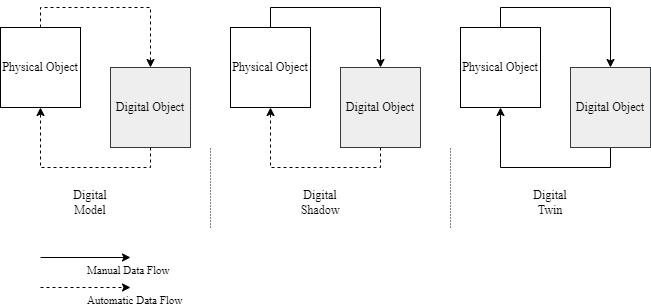
\includegraphics[width=0.8\textwidth]{figures/kritzinger.png}
  \caption{Comparison of Digital Shadow (DS), Digital Model (DM) and Digital Twin (DT) as presented by Kritzinger (2018). This distinction is crucial for understanding validation requirements across different digital representation types.}
  \label{fig:Kritzinger}
\end{figure}

The DM represents the most basic form. It contains manual data connections between physical and digital entities. These connections can be temporarily shifted or even disconnected. There is no control of the digital object over the physical entity. It rather is a simple or complex model \textit{describing} the modelled object. It can not make decisions by itself to influence the physical object. The reason lies in the potential outdated data the digital part possesses or in the fact that it does not contain logic to control the data flow back to the physical part by itself. The control and the obligation to interpret the results is completely in the hands of the modeller.
The DS is a more advanced version of the DM. It is a digital representation of the physical object, which is continuously updated with real-time data. The DS can be used for monitoring, analysis and simulation purposes. It can predict the future state of the physical object based on the current state and historical data. However, the DS is not able to influence the physical object. The control is, similar to the DM, still in the hands of the modeller. A DS is mainly used for simulation and in the literature often confusingly classified as a DT.
The DT is the most advanced version of the triplet. It is a digital representation of the physical object, which is also continuously updated with real-time data. The DT can be used for monitoring, analysis, and \textit{control} purposes. It can predict the future state of the physical object based on the current state and historical data. The DT can also influence the physical object by sending control signals to it. The control is partially or completely in the hands of the DT. The DT thus \textit{can} serve more purpose than modelling or simulating the physical object. It may serve as an autonomic system, updating itself or by help of the modeller \parencite{kritzinger2018digital}.

Digital twins are applied across various sectors, including manufacturing, defense, automotive, and recycling. This thesis focuses on manufacturing, particularly discrete material flow systems (DMFS). These systems process discrete objects (parts) that move along transportation routes or conveyor lines—either at regular or irregular intervals—integrating both production and logistics operations \parencite{arnold2005materialfluss, schwede2024learning}. A core simplification in their modeling is the abstraction of material flow as a sequence of discrete events, similar with the principles of discrete-event simulation (DES) \parencite{kovacs2016mathematical, robinson2014simulation}. DES is particularly well-suited for analyzing complex systems where state changes occur at discrete points in time, such as arrivals, departures, and processing steps \parencite{robinson2014simulation}.

In hindsight, DM played a crucial role in the design, planning, and control of DMFS, primarily through applications such as material flow simulations, logistic assistance systems, and digital factory implementations \parencite{Thiede2013}. However, advancements in both DS and DT have enabled a revolution from isolated, usecase-specific models toward complete digital models that span the entire lifecycle of DMFS \parencite{Abdoune2023}. This transition is largely driven by the increasing demand for predictive capabilities by stakeholders and automated decision support in manufacturing systems, reflecting the cornerstones of Industry 4.0 \parencite{frank2019industry}.

In practice, the automated data transfer between the digital model and the physical system is of secondary importance for DMFS management. Unlike in time-critical applications, human decision-makers remain an integral part of the control loop, ensuring that real-time automation is not always necessary \parencite{schwede2024learning}. Consequently, for this thesis, digital simulations and digital twins will be treated as equivalent concepts.

Beyond merely replicating the current state and managing historical data, digital twins serve a crucial function in predicting system behavior and evaluating potential modifications. The widespread adoption of DES within digital twins highlights the central role of simulation-based digital twins (SBDT) in DMFS \parencite{Lugaresi2021aifac}. As \citeauthor{schwede2024learning} emphasize, SBDTs provide decision support for optimizing cost and performance in highly competitive manufacturing environments. While current SBDTs are primarily developed and updated manually by domain experts, emerging research explores how machine learning (ML) can enhance predictive accuracy and automate model updates by automatically learning model characteristics, reducing costs and development time from data.

Thus, the progression from digital models to simulation-based digital twins reflects an ongoing shift towards data-driven, predictive, and increasingly automated representations of DMFS, ensuring more informed decision-making throughout the whole system lifecycle \parencite{boschert2016digital,lim2020state}.

\section{Problem}
Despite the immense transformative potential of DT, their implementation comes with significant challenges. The creation and maintenance of accurate Digital Twins require substantial investments in technology and domain knowledge. This investment yields no return if the resulting model fails to accurately represent the modelled entity or delivers incorrect results. Automatic generation may be an elegant solution, but posesses the risk of learning edge cases, ignoring the main trend. Manufacturing data used as training data must be preprocessed and cleaned thoroughly. The DT per definition has to be able to perform real time decision making without time lags. This yields the requirement to extract, transform, clean and load (ETL process, \cite{vassiliadis2002conceptual}) data on the fly, performing inference fully in memory. All these hurdles happening daily are challenges to automatic learning \parencite{ribeiro2016should,zhao2024data}. As industries integrate DT into their production processes, establishing trust becomes fundamental as well \parencite{trauer2022digital,arrieta2020explainable}. To gain widespread acceptance, the technology must demonstrate accuracy, transparency, and cost-efficiency \parencite{Wright2020amse,Shao2023mfglet}. Without these qualities, organizations will likely fall back to familiar methods, potentially building resistance to technological advancement \parencite{lapointe2005multilevel}.

Even if the automatic learning of the DT was performed sucessfully, the question of its correctness, precision and robustness remains unanswered. These questions are solved by validation, verification and uncertainty quantification frameworks (VVUQ) \parencite{sel2025survey}. Ensuring the validity, reliability, and accuracy of a Digital Twin is critical, yet traditional V&V approaches rely heavily on manual expert involvement and case-specific reference values \parencite{Bitencourt2023,hua2022validation}. This creates inefficiencies, particularly in the context of automated DT generation, where such manual processes conflict with the goal of reducing development effort. \cite{hua2022validation} even argue that there are no state of the art VVUQ methods for Digital Twins. One hurdle to standardized VVUQ frameworks is the lack of a clear definition for validity and verification in the context of Digital Twins \parencite{Bitencourt2023}.

For discrete material flow systems, these challenges are even more stressing due to their processual nature and inherent stochastic elements. Manufacturing processes may fail due to anomalies, resource constraints or human error. VVUQ approaches have to anticipate these risks. When DT for these systems are generated automatically, conventional validation approaches become problematic, as they negate much of the efficiency gained through automation. This creates an apparent paradox: Automated Digital Twin generation reduces initial development effort but potentially increases subsequent validation complexity, mitigating efficiency gains through automation. State of the art VVUQ frameworks have to uphold the efficiency gains earned while ensuring validity and reliability of the Digital Twin.

\section{Objective of the Thesis}
% This section includes: Motivation, Relevance, Research Questions, and Hypotheses

The thesis thus addresses this paradox by developing a data-driven framework for automated VVUQ of automatically generated, simulation-based DT which have been learned from data. The focus lies on DMFS due to their practical relevance and dynamical, processual nature. The endeavor can further be concretized by the following research questions (RQ):

\begin{itemize}
  \item \textbf{RQ1:} How can automated validation and verification processes for digital twins be efficiently implemented?
  \item \textbf{RQ2:} Which data-driven approaches are best suited to identify discrepancies between simulated behavior and real operational data in discrete material flow systems?
  \item \textbf{RQ3:} To what extent does the developed framework improve the quality and reliability of digital twins compared to traditional V&V methods?
\end{itemize}

This thesis addresses these questions by proposing that object-centric event logs—the same data structures often used to generate DT in manufacturing—can serve as the foundation for an automated, use case-independent validation and verification framework. Such an approach would maintain the efficiency benefits of automated generation while ensuring the resulting Digital Twins meet necessary quality standards. The development and monitoring of situative reference values which can not be generalized across all DTs is a key aspect of this approach. The framework will be evaluated using a case study from the discrete material flow domain, providing empirical evidence of its effectiveness in improving model accuracy and efficiency.

% This section includes: Motivation, Relevance, Research Questions, and Hypotheses
% Content goes here

Das Hauptziel dieser Arbeit ist die Entwicklung eines datengetriebenen Frameworks zur automatisierten Verifikation und Validierung von digital generierten, simulationsbasierten digitalen Zwillingen. Der Fokus liegt dabei auf diskreten Materialflusssystemen, da diese aufgrund ihrer Komplexität und Dynamik besondere Herausforderungen hinsichtlich der Modellgenauigkeit und Prozesssynchronisation aufweisen.
\section{Structure of the Thesis and Methodological Approach}
% Content goes here


\section{Problem}

Trotz des hohen Potenzials digitaler Zwillinge treten in der Praxis zahlreiche Herausforderungen auf. Die automatisierte Erstellung simulationsbasierter Modelle birgt das Risiko, dass wesentliche Systemkomponenten oder Interaktionsmuster unzureichend erfasst werden. Dies führt zu Diskrepanzen zwischen dem digitalen Modell und dem realen System, was im schlimmsten Fall die Grundlage für fehlerhafte Simulationen und falsche betriebliche Entscheidungen bildet. Traditionelle Verifikations- und Validierungsprozesse (V\&V) basieren häufig auf manuellen Prüfungen, die angesichts der Komplexität und der Datenmengen in modernen Produktionssystemen nicht mehr effizient durchführbar sind \parencite{Kritzinger2018}.

Ein weiteres Problemfeld stellt die Integration von Echtzeitdaten in die Simulationsmodelle dar. Während historische Daten die Basis statischer Modelle bilden, erfordert die dynamische Anpassung digitaler Zwillinge die kontinuierliche Auswertung und Synchronisation aktueller Betriebsdaten. Dies führt zu Herausforderungen hinsichtlich der Datenkonsistenz, -qualität und -verarbeitung. Zudem fehlt es oft an standardisierten Bewertungsmetriken, die eine objektive Beurteilung der Modellgüte ermöglichen. Diese Probleme machen deutlich, dass herkömmliche V\&V-Methoden nicht ohne Weiteres auf automatisiert generierte, simulationsbasierte digitale Zwillinge übertragbar sind.

Insbesondere in diskreten Materialflusssystemen, in denen zahlreiche Prozessvariablen und Interaktionskomponenten eine Rolle spielen, erfordert die Sicherstellung der Modellgenauigkeit neue Ansätze. Es besteht daher dringender Forschungsbedarf, um datengetriebene und automatisierte V\&V-Methoden zu entwickeln, die den spezifischen Anforderungen solcher Systeme gerecht werden \parencite{Kritzinger2018, Uhlemann2017}.

\section{Objective of the Thesis}

Das Hauptziel dieser Arbeit ist die Entwicklung eines datengetriebenen Frameworks zur automatisierten Verifikation und Validierung von digital generierten, simulationsbasierten digitalen Zwillingen. Der Fokus liegt dabei auf diskreten Materialflusssystemen, da diese aufgrund ihrer Komplexität und Dynamik besondere Herausforderungen hinsichtlich der Modellgenauigkeit und Prozesssynchronisation aufweisen.

\subsection*{Motivation und Relevanz}

Die Motivation dieser Forschungsarbeit ergibt sich aus mehreren zentralen Aspekten:
\begin{itemize}
  \item \textbf{Effizienzsteigerung:} Durch den Einsatz automatisierter V\&V-Methoden können Modellabweichungen frühzeitig erkannt und behoben werden, was zu einer signifikanten Reduktion von Fehlerquellen und Optimierungspotenzialen in Produktionsprozessen führt.
  \item \textbf{Digitalisierung und Vernetzung:} Mit der zunehmenden Integration von IoT und Sensorik in Produktionsanlagen steigt die Verfügbarkeit von Echtzeitdaten, die in digitalen Zwillingen verarbeitet werden können. Ein zuverlässiges V\&V-Framework stellt sicher, dass diese Daten adäquat in die Modelle einfließen.
  \item \textbf{Wettbewerbsvorteile:} Unternehmen, die in der Lage sind, ihre digitalen Modelle präzise und effizient zu validieren, sichern sich langfristig Wettbewerbsvorteile in einem zunehmend globalisierten Marktumfeld \parencite{Grieves2014}.
\end{itemize}

\subsection*{Forschungsfragen und Hypothesen}

Die Arbeit fokussiert sich auf folgende Forschungsfragen:
\begin{itemize}
  \item Wie können automatisierte Prozesse zur Verifikation und Validierung von digital generierten, simulationsbasierten digitalen Zwillingen effizient implementiert werden?
  \item Welche datengetriebenen Ansätze eignen sich am besten, um Abweichungen zwischen simuliertem Verhalten und realen Betriebsdaten in diskreten Materialflusssystemen zu identifizieren?
  \item Inwieweit verbessert das entwickelte Framework die Qualität und Zuverlässigkeit der digitalen Zwillinge im Vergleich zu traditionellen V\&V-Methoden?
\end{itemize}

Es wird die Hypothese aufgestellt, dass ein integriertes, datengetriebenes V\&V-Framework signifikante Verbesserungen in der Modellgenauigkeit und Effizienz der Validierungsprozesse bewirken kann. Durch den Einsatz moderner Datenanalysen und maschineller Lernverfahren sollen systematische Abweichungen frühzeitig erkannt und Korrekturmaßnahmen automatisiert eingeleitet werden \parencite{Tao2018}.

\section{Structure of the Thesis und Methodological Approach}

Der Aufbau dieser Arbeit gliedert sich in mehrere Kapitel, die im Folgenden kurz vorgestellt werden:

\begin{itemize}
  \item \textbf{Kapitel \ref{chap:literature}:} Umfassende Literaturrecherche. In diesem Kapitel werden die theoretischen Grundlagen digitaler Zwillinge, bestehende Simulationsansätze und aktuelle V\&V-Methoden analysiert.
  \item \textbf{Kapitel \ref{chap:framework}:} Entwicklung des datengetriebenen Frameworks. Hier werden die konzeptionellen und architektonischen Entscheidungen, die Auswahl der Algorithmen und die Implementierungsdetails dargestellt.
  \item \textbf{Kapitel \ref{chap:caseStudy}:} Fallstudie. Anhand eines konkreten Beispiels aus dem Bereich der diskreten Materialflusssysteme wird das entwickelte Framework empirisch validiert.
  \item \textbf{Kapitel \ref{chap:evaluation}:} Evaluation. Die Ergebnisse der Fallstudie werden hinsichtlich Modellgenauigkeit, Prozesszeiten und Fehlerhäufigkeiten quantitativ und qualitativ ausgewertet.
  \item \textbf{Kapitel \ref{chap:conclusion}:} Zusammenfassung und Ausblick. Abschließend werden die wesentlichen Erkenntnisse zusammengefasst, Limitationen diskutiert und Perspektiven für zukünftige Forschungsarbeiten aufgezeigt.
\end{itemize}

Methodologisch basiert die Arbeit auf einem iterativen Entwicklungs- und Validierungsansatz, der sowohl qualitative als auch quantitative Methoden integriert. Zunächst erfolgt eine detaillierte Literaturrecherche, um den aktuellen Stand der Technik zu erfassen und bestehende Forschungslücken zu identifizieren. Aufbauend auf diesen Erkenntnissen wird das Framework in modularer Form entwickelt. Die einzelnen Module – etwa für Datenerfassung, -vorverarbeitung, Modellgenerierung sowie die automatisierte V\&V – werden zunächst unabhängig implementiert und anschließend in ein Gesamtsystem integriert.

Ein zentraler Bestandteil der methodischen Vorgehensweise ist die empirische Validierung des Frameworks durch eine praxisnahe Fallstudie. Hierbei werden reale Prozessdaten eines diskreten Materialflusssystems herangezogen, um die Simulationsergebnisse kontinuierlich mit den tatsächlichen Betriebsdaten abzugleichen. Die Evaluation erfolgt durch die Analyse quantitativer Metriken (z. B. Abweichungsmaße, Reaktionszeiten) und wird durch qualitative Analysen ergänzt, um systemische Fehlerquellen aufzudecken \parencite{Uhlemann2017}.

Die Implementierung moderner Softwaretechnologien und datengetriebener Ansätze, wie etwa maschinelles Lernen, soll dabei helfen, die Validierungsprozesse zu automatisieren und flexibel an veränderte Betriebsbedingungen anzupassen. Der iterative Entwicklungsprozess ermöglicht es, das Framework kontinuierlich zu optimieren und auf die spezifischen Anforderungen unterschiedlicher industrieller Anwendungen zuzuschneiden. So wird ein dynamisches Instrument geschaffen, das nicht nur den theoretischen Anforderungen genügt, sondern auch in der Praxis anwendbar ist \parencite{Tao2018, Kritzinger2018}.

Zusammenfassend bietet diese Arbeit einen innovativen Beitrag zur Weiterentwicklung digitaler Zwillinge in diskreten Materialflusssystemen. Durch die Kombination theoretischer Fundierung, moderner datengetriebener Methoden und empirischer Validierung wird ein Framework vorgestellt, das signifikante Verbesserungen in der Modellgenauigkeit und Effizienz von V\&V-Prozessen ermöglicht. Die erzielten Ergebnisse tragen dazu bei, die Zuverlässigkeit digitaler Zwillinge zu erhöhen und bieten zugleich wertvolle Ansätze für die zukünftige Entwicklung in einer zunehmend digitalisierten und vernetzten Produktionslandschaft.

\chapter{Theoretical Foundation}
\label{chap:theory}

The following chapter provides a theoretical foundation for the research conducted in this thesis. It introduces the basic concepts of material flow planning and simulation, digital twins, process mining, and verification, validation, and uncertainty quantification (VVUQ). The relevance of these concepts in the context of simulation-based digital twins and their application in corporate practice will also be discussed.


\section{Discrete Material Flow Systems and Simulation}
This section begins with an introduction of the underlying concepts of DMFS and Simulation Based Digital Twins (SBDT).
\label{sec:material-flow}
\subsection{Basic Concepts}
DMFS cannot be fully understood without first clarifying the principles of Discrete Event Simulation (DES) for Discrete Event Systems. In DES, a system changes its state through \textit{events} that occur at specific, discrete time instances; it is assumed that no changes occur between two successive events. Consequently, the state of the system is completely defined by the values of its descriptive variables at each event occurrence \autocite{varga2001discrete}. The time at which an event occurs is typically marked by a timestamp, and the scientific observation of such systems is conducted by analysing the discrete \textit{sequence} of events over time \autocite{robinson2014simulation}.

Simulation, in this context, refers to the process of imitating the operation of a Discrete Event System over time—often through multiple event sequences. This imitation is captured in a model, and the core activities in a simulation involve constructing and experimenting with this model. A high-quality simulation abstracts the essential features of the system, which requires the modeller to have a sound a priori understanding of what “essential” means in the given context. Although the model can later be refined, its quality is primarily measured by its ability to predict outcomes and offer a diverse range of scenarios \autocite{maria1997introduction}.

In the context of DMFS, their simulation describes the imitation of material flow systems by breaking down continuous flows into discrete events. Such material flow systems can be characterized as “systems processing discrete objects (parts) that move at regular or irregular intervals along transportation routes or conveyor lines, comprising production and logistic systems” \autocite{Arnold2006,schwede2024learning}. These systems form the backbone of material flow planning and control structures. The central idea of material flow planning and control is to ensure that material requirements—both in terms of quantity and timing—are met during transportation and storage across the various stages of the supply chain \autocite{Gehr2007}. Importantly, the time horizon of interest spans from order placement up to delivery.
To summarize, DMFS are often simulated using DES, which abstracts the continuous flow of materials into discrete events. The simulation is carried out using a model. The simulation and modeller are embedded in the context of material flow planning and control, which aims to ensure that material requirements are met across the supply chain. Successfully performed material flow planning and control induce high quality data for simulation and modelling purposes.

\subsection{Comparing DMFS}
\label{sec:comparing-dmfs}
Because the simulation of DMFS often involves (discrete) event simulation, events in DMFS need to be further differentiated to be comparable. \Autocite{Arnold2006} propose to differentiate DMFS into static and dynamic components.

Static components describe the possible states of the system. Possible states can be the set of possible processes given a part or resource, for example. Dynamic components define the concrete material flow for a certain part or order.
Static components include parts, resources and processes \autocite{schwede2024learning}. Parts are transformed by processes using resources, sometimes based on orders. Transformation can have an impact on physical properties of the parts (transformation model), spatial position (transition model), the quality of the parts (quality model) and takes time (time model) and uses resources (resource model). Resources have a capacity of handling parts in parallel (resource capacity model) and processes have a predecessor-successors relationship (process model).
Dynamic components are used to define the concrete dynamic material flow within the DMFS. There are four components: Order generation, order control, resource control and supply control. Order generation defines the load the system must process. Order control defines how parts are processed, sometimes referred to as routing rules \autocite{mildeautomated}. Resource control defines how resources decide to handle processing requests, also sometimes referred to as priority rules. Supply control describes how supply parts are provided \autocite{mildeautomated,schwede2024learning}. See the latter source for a more detailed description of the components.


\subsection{Production Planning and Control}
\label{sec:ppc}
Successful companies use production planning and control frameworks to describe and optimize their DMFS. After establishing a theoretical foundation and simulation approaches for DMFS, this section thus focusses on Production Planning and Control (PPC) as a critical factor influencing the quality and quantity of data generated by Discrete Event Simulation.
PPC is the structured approach to planning, scheduling, controlling and managing all aspects of the manufacturing process. It involves the coordination of resources, processes, and orders to meet production goals. PPC is essential for optimizing production processes, reducing costs, and improving quality. The main functions of PPC include production planning, production scheduling, and production control. Production planning involves determining the production capacity, production goals, and production processes. Production scheduling involves creating a detailed schedule for production activities. Production control involves monitoring and controlling production activities to ensure that production goals are met \autocite{kiran2019production}. Scheduling is usually the last step performed before execution of the plan \autocite{pinedo2012design}.

The integration of PPC with simulation models is crucial because it directly affects the data quality used in DES of DMFS. Effective PPC processes anticipate anomalies in the production cycle, allowing for adjustments that maintain system efficiency and reliability. If successful, these adjustments yield high-quality data that enhance the accuracy of simulation outcomes. \autocite{kiran2019production}.


\subsection{Key Performance Indicators}
\label{sec:relevant-kpis}
Up to this point, DES for SBDT of DMFS has been introduced, outlining the key factors that contribute to a robust simulation. A model differentiation framework proposed by \citeauthor*{schwede2024learning} has been briefly presented to facilitate comparison of SBDT. Furthermore, the critical role of PPC in generating high-quality data for simulation has been discussed. These discussions ignored up till now that, even when SBDT are integrated within well-functioning PPC processes, various SBDT models remain prone to errors and inherent trade-offs that must be addressed by the modeller \autocite{Tao2018ijamt}.

The goal conflict of the modeller when developing SBDT can be described by the following conflict triangle \autocite{robinson2014simulation,balci2012life}:

\begin{figure}[htbp]
  \centering
  
\includegraphics[width=0.6\textwidth]{figures/goals.png}
  \caption{The goal conflict of the modeller when developing SBDT. Aiming for higher accuracy (validity) often leads to higher computational costs (efficiency) and reduced scalability (applicability). Reaching more efficiency often leads to reduced accuracy and scalability. Aiming for higher scalability often leads to reduced accuracy and efficiency.}
  \label{fig:goals}
\end{figure}

Focusing one of the three dimensions—accuracy (validity), efficiency (computation time), and applicability (scalability)—often leads to trade-offs in the other two dimensions. Oftentimes the data itself is not sufficient to make a decision on which trade-off to make. Limited data points may hinder the modeller from reaching high validity. System architecture may block the system from reaching good scalability. Hardware limitations may hinder the modeller from reaching high efficiency.
At other times, corporate management may have a preference for one of the dimensions.

One solution to balance and quantify these goals can be achieved by defining a set of KPIs. Some may already be available through PPC, some may be calculated from DES data or the DES itself. Optimally, the data warehouse provides relevant views \autocite{cui2020manufacturing}. Because the SBDT in theory mirrors the DMFS, the KPIs gathered from PPC and the DES should yield identical values. Deviations between the KPIs of the SBDT and the DMFS may indicate errors in the SBDT or anomalies in the DFMS. The following KPIs are relevant for the evaluation of SBDT:

\begin{figure}[htbp]
  \centering
  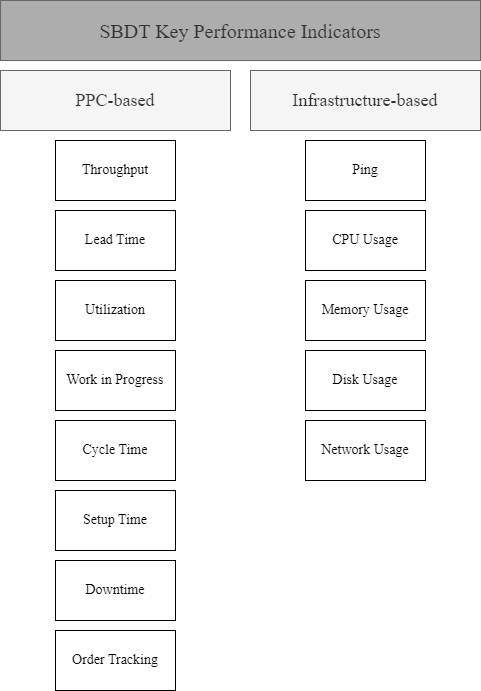
\includegraphics[width=0.8\textwidth]{figures/kpi.png}
  \caption{SBDT KPIs differentiated by PPC-based and Infrastructure-based indicators.}
  \label{fig:kpis}
\end{figure}

\begin{equation}
  \text{Throughput} = \frac{\text{Number of units produced}}{\text{Time period}}
  \label{eq:throughput}
\end{equation}

\begin{equation}
  \text{Lead Time} = \text{End time of the process} - \text{Start time of the process}
  \label{eq:lead_time}
\end{equation}

\begin{equation}
  \text{Cycle Time} = \frac{\text{Total processing time}}{\text{Number of units produced}}
  \label{eq:cycle_time}
\end{equation}

\begin{equation}
  \text{Total Setup Time} = \sum_{i=1}^{n} \text{Setup Time}_i
  \label{eq:setup_time}
\end{equation}

The PPC related KPIs may be provided by the above-mentioned data warehouse, because they are highly relevant in the context of production scheduling and control. \textbf{Throughput}, as defined in \autoref{eq:throughput}, measures the number of produced parts at the last station in a specified period and is an indicator for the productivity of the manufacturing system \cite{hopp2011factory, imseitif2019throughput}. \textbf{Lead time}, formulated in \autoref{eq:lead_time}, is the cumulative time a part travels through the system from start to finish and serves as an indicator for the efficiency of the manufacturing system \cite{slack2010operations, pfeiffer2016manufacturing}. \textbf{Cycle time}, shown in \autoref{eq:cycle_time}, measures the same duration as lead time but focuses only on the active production process, excluding transports and waiting times \cite{goldratt2004goal, griffin1993metrics}. \textbf{Setup time}, as expressed in \autoref{eq:setup_time}, measures the time needed to prepare a machine for a new task and is an indicator for the flexibility of the manufacturing system \cite{allahverdi1999review, allahverdi2008significance}. In the given use case, the thesis aggregates the setup time for all setup processes. All KPIs presented so far can be calculated dynamically when new data has been sent. Later on, they may serve as an alert system for the modeller to detect deviations between the SBDT and the DMFS, see \autoref{sec:vvuq-sbdt}.

The infrastructure related KPIs are derived by sensors from the executing system of the SBDT. Ping time measures the time needed to send a signal from one point to another. It is an indicator for the latency of the infrastructure \autocite{wu2021digital}. SBDT need to enforce real-time control over the physical entity. The latency thus needs to be as low as possible. In this scenario, one point (sender) is represented by the physical entity and its sensors. The receiving point runs the SBDT. It is advantageous to run the SBDT on Edge to minimize latency- and transmission costs \autocite{li2018learning}. CPU-, memory-, disk- and network usage metrics are indicators for the load of the infrastructure. They are important to detect bottlenecks in the infrastructure \autocite{li2018learning}. The first indicator is usually measured in percent of the maximum CPU capacity. The latter three indicators are usually measured in bytes or bits per second \autocite{granelli2021evaluating}. The framework derived in \autoref{chap:methodology} does not incorporate infrastructure-based KPIs.


\section{Digital Twin: Definition and Concepts}
\label{sec:digital-twin}
The latter section gave a short introduction into DFMS, DES, its metrics and the corporate processes accompanying the SBDT. Now, the thesis sheds light on the DT itself. For a short introduction to the topic, see \autoref{chap:introduction}.

Like introduced in the preceding chapter, DT inherent the highest order of modelling fidelity compared to DM or DS. There are different definitions of DT present in the literature \autocite{Negri2017promfg,zheng2019application,glaessgen2012digital,Demkovich2018def,boschert2016digital,grieves2014digital,kritzinger2018digital,Tao2018ijamt,zehnder2018representing}. Each of them highlights different aspects of the DT. This thesis utilizes the definition by \autocite{grieves2014digital} which highlights the conceptual elements of the twin and its lifecycle focus:

\begin{quote}
  The digital twin concept (...) contains three main parts: A) Physical products in real space, (B) virtual products in virtual space and (C) the two-way connections of data and information that tie the virtual and real products together. \autocite{grieves2014digital}
\end{quote}

The physical product is the entity which will be modelled. The virtual product is the DT itself, but also its infrastructure, for example data services making the real-time data flow possible \autocite{Tao2018ijamt}. The two-way connection is the data flow between the physical and the virtual product. The data flow is bidirectional. \citeauthor{zehnder2018representing} add that the data flow may contain meta data "describing the data source and its context". Also the connection protocol is of importance here (e.g. MQTT or REST). TCP may be the method of choice as it ensures that the packages arrive in the correct order and without errors \autocite{li2018learning}.

\subsection*{Types of Digital Twins}
\label{sec:types-digital-twins}
Now that a unified understanding of DT has been established, this section focuses on how DT may be learned from different sources of information. The following list includes the most relevant types of DT with a focus on different kinds of information sources:

\begin{itemize}
  \item Simulation-based DT (SBDT) \autocite{Lugaresi2021aifac,martinez2018automatic}
  \item Data-driven DT (DDDT) \autocite{he2019data,Friederich2022}
  \item Hybrid Digital Twins (HDT) \autocite{luo2020hybrid,huang2023hybrid}
\end{itemize}


SBDTs \autocite{Lugaresi2021aifac,martinez2018automatic,boschert2016digital} are based on DES. They utilize discrete event simulation (see \autoref{sec:material-flow}) to create a dynamic representation of the physical system \autocite{schluse2016simulation,pantelides2013online}. To incorporate a SBDT into workflows and processes, suitable data structures must be in place beforehand \autocite{boschert2016digital}. DES may improve the predictive capabilities of the model compared to manual twin creation. DES is able to model causal relationships between the events \autocite{francis2021towards}. In contrast, the development of a realistic simulation model requires experts and time \autocite{Charpentier2014}. If the simulation model fails to capture recent behaviour of the physical entity, a recalibration is mandatory \autocite{Friederich2022}. SBDTs are a step forward to speed up the creation and updating processes of DTs.

DDDT rely on the utilization of data to model the physical entity. The data may be gathered from sensors, data warehouses or other sources (later on developed framework summarizes this under the term data sources, see \autoref{sec:framework}). The data is used to train a model which represents the physical entity. The model may be a neural network, a decision tree or another machine learning model. The model is then used to predict future states of the physical entity. The model may be updated with new data to increase its accuracy \autocite{he2019data,Friederich2022}. For a more detailed description of DDDT including its up- and downsides, see \autoref{sec:data-driven-digital-twins}.

HDT combine different sources of information to create a more accurate model of the physical entity. The sources may be simulation models (see \autoref{sec:material-flow}), data-driven models (see \autoref{sec:data-driven-digital-twins}) or physics-based models. Physics-based models contain information about the physical properties and behaviours of the entity. They do not have to learn these characteristics from the data because this information is made available to the model \textit{a priori} \autocite{kapteyn2022data,aivaliotis2019methodology}. The simulation based models accompanying the physics-based one obeys characteristics of SBDT, see above. The combination of different sources may make the HDT more robust and a faster learner. HDT unite the advantages of SBDT with the knowledge advantage physics based models have. Unfortunately, they also inherit the disadvantages of SBDT through their simulation character. Physics-based models may also involve heavy involve heavy computational costs and domain expertise \autocite{kapteyn2022data}.

\subsection*{Data-Driven Digital Twins}
\label{sec:data-driven-digital-twins}

While SBDTs and HDT possess significant computational costs and require domain expertise, DDDT are able to learn from data without the need for a hand-written simulation model. The DDDT \textit{learns} the model. Learning in the context of DDDT is not trivial, several approaches have been proposed in the literature \autocite{he2019data,Friederich2022,francis2021towards}. Often times Data Science methods come to work. The learning process may be supervised or unsupervised. Supervised learning uses labelled data to train the model \autocite{cunningham2008supervised}. The label can symbolize different values of interest. Unsupervised learning uses unlabelled data to train the model \autocite{barlow1989unsupervised}. Often times, the task at hand is to group the data into different categories, see \autoref{sec:knn} \autocite{Biesinger2019}.
The learning process may be online or offline. Offline learning uses the data \textit{once} for training, validation and testing, while online learning continuously updates the model with new data to adapt to changes in the physical system. Online learning is thus able to capture new trends in the data and to foresee concept drift \autocite{tsymbal2004problem}. DDDT have to be differentiated from data-driven simulation \autocite{Charpentier2014}, which involves human intervention to create highly individual solutions for the physical entity. The key difference is that every characteristic has to be explicitly described in the model by the expert, there are no efforts to let an intelligent algorithm learn these by itself. DDDT may be able to update themselves to new trends in the data by online learning, termed \textit{synchronization} \autocite{reinhardt2019survey}. Latter has to be differentiated from \textit{updating}, which is a manual process to take corrective action in the logic of the twin itself \autocite{schwede2024learning}. An example for updating a DDDT may be the addition of a new feature to the model. An example for synchronization may be the adaption of the model to new trends in the data. The latter may be done by the model itself, the former has to be done by the modeller.
DDDT thus rely less on domain expertise and manual model creation. A suitable model may be able to capture relevant trends in the data and to predict outcomes which describe most of the characteristics of the physical entity. \autocite{francis2021towards} propose several elements a DDDT must contain to be termed \textit{data-driven}:

\begin{enumerate}
  \item \textbf{Data Collection:} The relevant entities to be modelled have to be identified. This activity involves data gathering of the identified entities and ensuring a steady data stream to a database. The data may be gathered from sensors, data warehouses or other sources.
  \item \textbf{Data Validation:} This step involves cleaning and preprocessing the data. The data may contain missing values, outliers or other errors. The data has to be cleaned and preprocessed to ensure a high quality of the model. Plausibility checks may be performed to ensure the data is correct.
  \item \textbf{Knowledge Extraction:} After the data has been collected and cleaned, events have to be detected. \Citeauthor{francis2021towards} utilize PM terms in this context, such as event detection and process discovery. The main goal in this step is to find a common ground on which events are of interest. The thesis later dives deeper into PM techniques applied here, see \autoref{sec:process-mining}.
  \item \textbf{(Semi-)automatic Simulation Modelling:} The data is used to train a model. This step may use offline or online data as a stream. The model may be a neural network, a decision tree or another machine learning model. The model is then used to predict future states of the physical entity. The model may be updated with new data to increase its accuracy.
  \item \textbf{Continuous Model Validation:} Interestingly,\citeauthor{francis2021towards} propose a continuous model validation. In the online learning case, they recommend to use the steady data stream to apply validation techniques continuously, see \autoref{sec:vvuq-sbdt} The validation may be performed by comparing the model predictions with the real data. If the model deviates from the real data, the model may be recalibrated.
\end{enumerate}

DDDTs go one step further than SBDT and minimize the influence of the human in the loop \autocite{francis2021towards,Friederich2022}. Faster model development and updating activities are the result. The third reason to automate DT endeavours elaborated by \citeauthor{schwede2024learning}, increasing prediction quality, rises and falls with the data quality, thus the gathering and preprocessing efforts of the modeller. Extrinsic factors like the number of data points available also play into the equation. If the number of features is greater than the number of samples, the curse of dimensionality hinders a good modelling performance \autocite{koppen2000curse}. DDDT should avoid biased or noisy predictions at all costs. The identification of \textit{relevant} events poses the risk of introducing a selection bias, rather a confirmation bias. The modeller may have the tendency to select events which confirm his or her hypothesis. Random sampling may be a solution to this problem, but can destroy sequential information patterns in event sequences. Overall DDDT are a promising approach to model the physical entity. If the right balance between human involvement and automated learning is found, it may be an efficient solution \autocite{francis2021towards}. Thinking one step ahead, employing data-based VVUQ approaches may also be a step forward. This topic will be discussed in Section \autoref{sec:ml-approaches}.

\label{par:asmg}
One last discipline, automatic simulation model generation (ASMG), is worth mentioning. ASMG has to be differentiated from DDDT by the effort to automatically generate models, thus DM and DS through DES. Automatic DT generation is not necessarily the goal. It aims to automate the model generation process and tries to eliminate the human in the loop, \autocite{reinhardt2019survey,lechevalier2018methodology}. Automation is achieved by taking into account a diverse range of data sources, including Computer Aided Design data, PPS data, production manuals, process data and programming code, thus reaching a high data variability. The gathered data has to be processed online or offline as well through suitable frameworks or human intervention. Challenges lay in incomplete data \autocite{bergmann2014automatische}, although the same problems of DDDT also apply here. If the gained data is not mined thoroughly, human intervention is needed again, mitigating automation efforts.

To conclude this section about DT, the thesis summarizes that there are different types of DT differentiated by their source of information retrieval. A lot of work has been done to make the DT creation, updating and prediction process more efficient. By the help of simulation, data and automated model generation, the DT may be created with less time and resources than manually.

\section{Process Mining and Event Logs}
\label{sec:process-mining}
After introducing the corporate embedding of DTs and their types, the thesis now focusses on process mining (PM) and event logs. PM is a discipline which aims to extract knowledge from event logs. Event logs are the data basis for PM. The following section introduces the basic concepts of PM and event logs.

\subsection{Core Concepts}
\label{sec:core-concepts}
PM is a discipline established 1999 which is interdisciplinary rooted in the field of Data Science and Process Science \autocite{van2016data}. Data Science can be considered a process agnostic discipline \autocite{van2016data} while process science uses models not covering hidden trends in the data. The bridge between both approaches is PM. The goal of PM is to use event data to identify and extract process information \autocite{vanderAalst2012}. This information is used to discover (process discovery), monitor (conformance checking) and improve processes (process enhancement) \autocite{vanderAalst2012} by using event logs. Such logs must contain a case ID, an activity name and a timestamp. Additional information like resource information, order information or other context information may be added to the log \autocite{vanderAalst2012}. Such logs assume that the process can be captured fully and sequentially.

\begin{table}[htbp]
  \centering
  \caption{A fragment of a manufacturing event log: Each line corresponds to an event. The case ID groups unique events which are identified by an event ID to one group, a trace. The timestamp refers to the time of event occurrence, while the activity describes the event. In this example, additional information like resource name and cost are given as well. Case 1, for example, consists of five events, involving a warehouse, two inspectors, and one machine.}
  \label{tab:manufacturinglog}
  \resizebox{\textwidth}{!}{%
    \begin{tabular}{r r l l l r}
      \toprule
      \textbf{Case id} & \textbf{Event id} & \textbf{Timestamp} & \textbf{Activity}     & \textbf{Resource}  & \textbf{Cost} \\
      \midrule
      1                & 101               & 10-01-2025:08.00   & receive raw material  & Warehouse A        & 500           \\
                       & 102               & 10-01-2025:08.30   & initial quality check & Inspector Stefan   & 300           \\
                       & 103               & 10-01-2025:09.00   & cutting process       & Machine X          & 800           \\
                       & 104               & 10-01-2025:09.45   & assembly              & Worker Paul        & 600           \\
                       & 105               & 10-01-2025:10.30   & final inspection      & Inspector Eva      & 400           \\
      \midrule
      2                & 201               & 11-01-2025:07.45   & receive raw material  & Warehouse B        & 500           \\
                       & 202               & 11-01-2025:08.15   & cutting process       & Machine Y          & 800           \\
                       & 203               & 11-01-2025:09.00   & welding               & Robot Arm Z        & 700           \\
                       & 204               & 11-01-2025:09.45   & quality assurance     & Inspector David    & 400           \\
      \midrule
      3                & 301               & 12-01-2025:06.30   & receive raw material  & Warehouse C        & 500           \\
                       & 302               & 12-01-2025:07.00   & initial quality check & Inspector Claudius & 300           \\
                       & 303               & 12-01-2025:07.30   & CNC machining         & Machine W          & 900           \\
                       & 304               & 12-01-2025:08.15   & painting              & Worker Daniel      & 500           \\
                       & 305               & 12-01-2025:09.00   & packaging             & Worker Johannes    & 350           \\
      \bottomrule
    \end{tabular}%
  }
\end{table}

\autoref{tab:manufacturinglog} illustrates the PM concepts. The case ID groups unique events which are identified by an event ID to one group, a trace. The timestamp refers to the time of event occurrence, while the activity describes the event. In this example, additional information like resource name and cost are given as well. Cases containing the same events identified by unique event IDs will have different case IDs \autocite{van2016data}. Process discovery may try to produce a process model from the event log. The model may be a Petri net, a BPMN model or another process model. The challenge lies not in the recording of every trace present in the event log, rather in finding a generic representation of the most occurring traces. The process model must be generic enough to describe most traces, but specific enough to not get invalidated by future traces which may contain completely different events. Another major building block of this process model is accounting for trace concurrency. When several events may be identified to happen in parallel during the same time window, the model must recognize this. It can be spoken of a classical bias-variance trade-off lend from data science. The process most contain the most frequent traces but has to filter out traces which contain anomalies. Such anomalies like longer time per event due to a fire alarm have to be accounted for. Conformance checking may compare a given process model against a given event log. They are specialized in detecting aforementioned anomalies. A key insight in conformance checking lies in two possible deviations from reality: The given model does not capture the real behaviour (A) or reality differs from the model (B). In the first case, the model is not working as intended. In the second case, the event log is corrupt. The third view on event logs, process enhancement, enables the modeller to use the generated process model to identify bottlenecks. Anomalies identified serve as a good starting point because they reveal errors in the process sequence. The given table offers costs associated to each event ID. This information may be used to create an event benchmark to further optimize the desired "ideal" trace. The first goal of course is to ensure that no mistakes happen during a process.

More generally, PM empowers the modeller to perform VVUQ of an process model, event log or described trace. This concept is captured by the terms \textit{Play-In}, \textit{Play-Out} and \textit{Replay} \autocite{damm2001lscs}, see \autoref{fig:playinoutreplay}.

\begin{figure}[htbp]
  \centering
  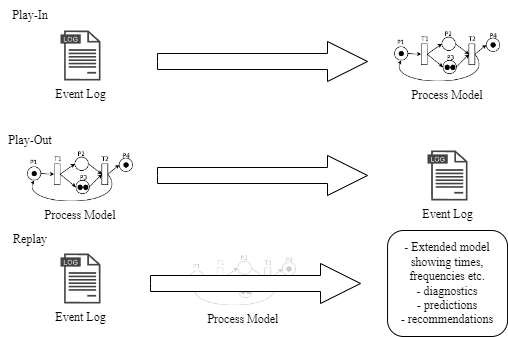
\includegraphics[width=0.8\textwidth]{figures/playinplayoutreplay.png}
  \caption{The Play-In, Play-Out and Replay concept in the context of PM. The Play-In phase involves the creation of a process model from an event log. The Play-Out phase involves the creation of an event log from a process model. The Replay phase involves the modification of the process model thorough information gained from the event log.}
  \label{fig:playinoutreplay}
\end{figure}

Play-In refers to the creation of a process model out of an event log. Play-Out may be called "sampling" in data science as it generates traces out of the model. DES uses Play-Out to generate new exemplary behaviour, see \autoref{sec:material-flow}. Here, a process model may be used to play-out (simulate) several traces of the desired events and then use bagging techniques like averaging the durations per event to gain robust KPIs (\autoref{sec:relevant-kpis}) and to reduce variance. A biased process model may still generate biased KPIs. Replay uses event log and process model together to check conformance, enriching the model with information captured in the log or to transform a descriptive process model into a prescriptive one \autocite{van2016data}.

PM uses different formats to display process models like petri nets and BPMN models, among others \autocite{vanderAalst2012}. The thesis at hand focusses on DDDT in the context of simulation. Such data-driven models often come as a black box, thus they can not be rendered by PM models.

\subsection{Object-Centricness in Process Mining}
\label{sec:object-centric-event-logs}

The problem with traditional PM lies in its single dimensionality of perspective. For each process analysis, a new play-out has to be performed. Interactions between different objects are not captured \autocite{van2023object}. One event may be related to different cases (convergence) or from the perspective of a case, there may be several equal activities within a case (divergence) \autocite{van2019object}.
Recently, object-centric event data (OCED) have been proposed as a new data basis for PM \autocite{van2019object}. OCED logs (OCEL) are a generalization of classical event logs. Such traditional event logs use the case ID as a label to group and distinguish events. They assume that the process model describes the start and end of a single object. Each event refers to exactly one object (case) \autocite{van2023object}. OCED overthrows these assumptions by assuming that events may relate to multiple objects. To account for this new logic, OCEL coins the terms events, objects, types, attributes and qualifier. Each object has exactly one object type. Several objects may have the same type. An object type can be a description of the function such as machine, customer, supplier or activity descriptions such as invoice, request. Objects are instances of these types. Events in particular have an event type, termed activity. The same non-uniqueness applies here\textemdash many events can have the same type like "processing complaint", "cooking coffee". Each event is described by exactly one type. OCED assumes event atomicity; each event is indivisible. Each event has one timestamp. Compared to traditional PM, events may relate to multiple objects through a qualifier (event to order\textemdashE2O). Such a qualifier may be, considering the event "printing label" and object "printing station", the label to be printed. Objects may be related to multiple objects (order to order\textemdashO2O). O2O relationships are frozen (static) and are assumed to not change. The O2O relationship may be used to describe the order of producing a product. For example, the O2O relation "main pcb to gyroscope" may say that the main pcb has to be produced before the gyroscope. Another O2O relation can be an order, the connection between the customer object and the ordered product. It is worth mentioning that objects can also be related indirectly together through two E2O relations: The E2O relation "producing" may connect the event "machine 1 produces" with the object "gyroscope". The E2O relation "check" may connect the event "machine 1 checks" with the object "main pcb", thus connecting the two objects "gyroscope" and "main pcb" indirectly via two events \autocite{van2019object}. E2O relations are dynamic. They may change over time, involving different objects. In the given example, "main pcb" would be checked with "display" instead of "gyroscope".

Events and objects have attributes (keys), possessing values. Event attribute values refer to exactly one event and one event attribute, they are not shared. For example, the cost for one event may have the value $10€$. The same logic applies to objects as well, one event attribute value refers to exactly one object and one object attribute. Because several events may have the same type and several objects may have the same type as well, each event- or object type may refer to any number of event or object attributes. They open interpretative possibilities for the modeller by considering them as expected attributes for the event or object type. The given example may be the event type "producing" which may have the event attribute "duration" and "cost". The object type "gyroscope" may have the object attribute "weight" and "size". One may average the different object attribute values of one type cluster to generate object type KPIs. A key specificity of object attribute values lies in the fact that they have a timestamp. Event attribute values do not. Latter information would be redundant because events to already have a timestamp, see above. Event attribute values may have cardinality one per event. $N$ event attributes have $n$ values. This does not apply to object attribute values. They may have multiple values because of their nature to change over time \autocite{van2023object}. This is why each object attribute value has a timestamp. The attribute value is in conclusion unique for a given object during a given time given one attribute. The given example may be the object attribute "weight" of the object "main pcb" which may change over time. The object attribute value "weight" may have the value $100g$ at time $t_1$ and $120g$ at time $t_2$.

OCEL thus extends traditional PM by accommodating the  multi-object nature of complex processes. Unlike classical event logs—which restrict events to a single case—OCEL captures dynamic interactions among multiple objects via E2O relations and static inter-object dependencies through O2O relations. This enriched framework enables a more comprehensive representation of real-world processes, where events may concurrently affect several objects. Timestamped object attribution values enable the modeller to perform temporal analysis and KPI derivation (\autoref{sec:relevant-kpis}). Overall, OCED provides a more detailed, semantically rich representation of complex, interconnected processes. \autocite{van2023object}.

\subsection{Process Mining as Enabling Technology}
\label{sec:process-mining-enabling-technology}

PM uses event logs to develop process models or to enhance existing ones, so these logs may serve as a foundation for VVUQ of models in general. Live twin data often can be exported to the event log format. Several standardizations have been proposed, with the IEEE XES standard being the most widely used \autocite{van2016data}. The XES standard defines a common format for event logs, enabling the exchange of event data between different software frameworks. The idea lies in exporting twin decisions or live data as event logs and then use PM tools to perform VVUQ.
Replay may be used on SBDT simulated traces in comparison with actual event data to reveal mismatches in sequences or timing. For example, the SBDT could have predicted a circular process. Replay can be applied to further analyse this bottleneck. Play-Out can empower the modeller to sample a big amount of exemplary traces to gain KPIs. OCED object attribute values may offer even more insights.
PPC systems (\autoref{sec:ppc}) often times deliver even more data to enrich the event log so that VVUQ can be performed easier. If event log extraction out of the SBDT is performed online, VVUQ can be performed on the fly. Both sources of information are incorporated in the framework, see \autoref{sec:framework}.

\section{VVUQ in the Context of Simulation-Based Digital Twins}
\label{sec:vvuq-sbdt}

The previous sections introduced the concepts of DES, PPC, relevant KPIs, DT, PM and OCED. This section now focusses on VVUQ in the context of SBDT. The thesis at hand uses the term VVUQ to describe the process of verifying, validating and quantifying the uncertainty of a SBDT. V\&V has a long history in manufacturing and DES \autocite{Bitencourt2023}. \Autocite{sel2025survey} add uncertainty quantification as a main interest. Their framework is applied in the medical domain, but they mention reasonable arguments regarding efficiency and safety of SBDT in general.\footnote{To go into detail, they deem erroneous data through sensor failure, model opacity (\autoref{sec:requirements-automatically-generated-models}) and the speed of model self-adaption as the necessities for UQ.} Thus, the thesis considers VVUQ instead of merely V\&V efforts. The following section introduces the basic concepts of VVUQ and its relevance for SBDT.


\subsection{Development process of VVUQ Concepts}
\label{sec:historical-development}
With the uprising of simulation models in the early 1950s \autocite{evans1967simulation}, the need for VVUQ arose unknowingly to the modellers. The usability of such simulations was deemed high as long as the results were promising, increasing trust in the technology \autocite{durst2017historical}. Blind trust does not validate models. Contrarily, if the results more or less were satisfactory, the model was considered validated \autocite{bonani2003physics}.

The first effort to define and perform verification was performed by \autocite{machlup1955problem} defining verification as "including the correctness of mathematical and logical arguments, the applicability of formulas and equations (...), the reliability and exactness of observations, the reproducibility of experiments, the explanatory or predictive value of generalizations.". \Autocite{naylor1967verification} further refined this definitions by introducing the idea of "goodness of fit". Latter describes the capability of the model to correctly reflect the modelled system. During the 1970s, researchers like Schlesinger \autocite{schlesinger1979terminology} defined validation as achieving a "satisfactory range of accuracy consistent with the application", while Ignall argued for validation against simulations rather than analytical models \autocite{ignall1978using}. Sargent's work from 1979 to 1984 proposed methods like user collaboration and independent verification and validation (V\&V), detailing techniques such as sensitivity analysis and Turing tests \autocite{Sargent2010wsc}. Balci developed a taxonomy and emphasized continuous V\&V, reflecting the need for ongoing assessment \autocite{balci2012life}.

By 2004, modern V\&V emerged. Considering model fidelity of today's approaches, \autocite{Oberkampf2004amr} introduced widely recognized definitions of V\&V:

\begin{quote}
  \textit{Verification} is the process of determining that a model implementation accurately represents the developer's conceptual description of the model and the solution to the model.

  \textit{Validation} is the process of determining the degree to which a model is an accurate representation of the real world from the perspective of the intended uses of the model. \autocite{Oberkampf2004amr}
\end{quote}

Verification thus concerns itself with the correctness of the given model \autocite{Sargent2010wsc}, while validation evaluates the quality of explanations quantitively \autocite{Oberkampf2004amr}. \Citeauthor{iso2017systems} span the concept of validation to computational models, where valid models correctly reflect the users intended functionality. PPC may provide the modeller with relevant KPIs to assess both.

\label{sec:uncertainty-quantification}
Uncertainty quantification (UQ) is a relatively new field in V\&V. It aims to quantify the uncertainty of the model and its predictions through the whole lifecycle of the model, including training, inference and prediction \autocite{sel2025survey}. Uncertainty quantification empowers the modeller to define confidence intervals to correctly emphasize the stochastic nature of the model predictions \autocite{volodina2021importance}. This is crucial for SBDT, where real-time decisions rely on accurate representations, as \autocite{francis2021towards} highlights the need for continuous updates. UQ differentiates \textit{aleatory} uncertainty, which is inherent to the data, and \textit{epistemic} uncertainty, which is due to lack of knowledge \autocite{sel2025survey}. Aleatory uncertainty may arise due to sensor errors in the physical entity, generating noise. Epistemic uncertainty may arise due to lack of data or knowledge about the physical entity \autocite{thelen2023comprehensive}. Epistemic uncertainty can be reduced. \Autocite{abdoune2022handling} provide a comprehensive overview of UQ challenges and potential solutions in the context of SBDT.

For SBDT, VVUQ is not a one-time activity but a continuous process (\autoref{sec:framework}), ensuring digital twins mirror physical systems accurately. This is vital for industries like manufacturing, where decisions based on digital twins have significant implications \autoref{sec:problem}.
The historical development of VVUQ, from early verification to integrated UQ, reflects the growing complexity of simulation models. As SBDT become central to decision-making, robust VVUQ practices ensure reliability, linking back to foundational concepts introduced earlier, see \autoref{sec:types-digital-twins}. The concepts of VVUQ are embedded in the context of PM and OCED, which may further assist described endeavours. Especially for UQ, PM offers a rich data source to quantify uncertainty and validate models by providing a \textit{degree of fit} of the given process model.


\subsection{VVUQ for Automatically Generated Models}
\label{sec:requirements-automatically-generated-models}
AMG stem largely stem from the DES discipline (\autoref{par:asmg}), termed automatic simulation model generation, ASMG \autocite{mildeautomated,Charpentier2014}. They may use data-driven techniques which reduce the manual effort to create and update themselves. These models adapt quickly to changing conditions, making them valuable for dynamic environments like manufacturing. However, ensuring their reliability requires specific VVUQ. Because ASMG models often are black boxes, traditional VVUQ methods may not be applicable. The challenge lies in understanding the model's internal logic and ensuring it accurately reflects the physical system. If sophisticated data driven methods have been applied, several \textit{key challenges} arise, hindering successful VVUQ:

\begin{itemize}
  \item \textbf{Model Opacity:} ASMG models often use sophisticated machine learning algorithms like neural networks. Such black-box models are difficult to interpret, making it hard to understand their internal logic. This opacity may hinder VVUQ, as the modeller cannot easily identify errors or biases.
  \item \textbf{Data Dependency:} Data-driven models rely on high-quality data. If the data is biased or noisy, the model's predictions may be inaccurate.
  \item \textbf{Dynamic Model Adaptation:} Models that continuously learn and adapt, such as those employing online learning, require ongoing validation to ensure they remain valid as new data is ingested. This dynamic nature introduces the risk of concept drift \autocite{lu2018learning}, where the underlying process changes over time, potentially degrading model performance.
  \item \textbf{Quantifying Uncertainty:} Model predictions are stochastic in nature. For applications where precision is crucial, such as in manufacturing, uncertainty needs to be quantified.
\end{itemize}

To assess these challenges, the thesis defines the following \textit{key requirements} for VVUQ of automatically generated models, especially SBDT:
\begin{itemize}
  \label{par:key-requirements}
  \item \textbf{Model Interpretability:} \label{par:surrogate} Ensuring the model's internal logic is transparent and understandable, enabling the modeller to identify errors or biases. Developing and employing techniques to make the decision-making processes of automatically generated models more transparent is crucial for VVUQ. Explainable AI methods, such as SHAP (SHapley Additive exPlanations, \autocite{lundberg2017unified}) or LIME (Local Interpretable Model-agnostic Explanations, \autocite{ribeiro2016should}), can help shedding light on model behaviour, facilitating verification efforts. This is particularly important for black-box models like deep neural networks, where understanding the reasoning behind predictions is challenging. Often times, it may be easier to use white-box models like decision trees or linear regression models, which are interpretable by design. Such models are often times labelled transparent models. If black-box models are instead chosen, so called \textit{surrogate models} may be used to approximate the black-box model. The surrogate model is a white-box model, which is easier to interpret. This approach is called \textit{post-hoc} explanation \autocite{fischer2024demystifying}.
  \item \textbf{Upholding Data Quality:} Implementing procedures to ensure that the data used for model generation and validation is accurate, complete, and representative of the operational environment is vital. This includes data cleaning, preprocessing, and plausibility checks to identify and mitigate issues like missing values, outliers, or biases. For instance, in manufacturing digital twins, sensor data must be validated for accuracy and consistency to ensure reliable model outputs \autocite{rodriguez2023updating}.
  \item \textbf{Validatable Algorithms:} Besides ensuring model interpretability, the algorithms used for model generation must be validatable. Security risks are a huge concern for companies employing SBDT into their processes \autocite{alcaraz2022digital}. The algorithms used have to be secure, hardened against attacks. This is especially important for online learning algorithms, which may be vulnerable to adversarial attacks \autocite{balta2023digital}. Manipulated data may lead to incorrect model predictions, causing severe consequences in safety-critical applications like autonomous driving or medical diagnosis. Ensuring the robustness of the algorithms is crucial for reliable VVUQ.
  \item \textbf{Continuous Validation:} VVUQ processes have to work in real-time to ensure the model remains valid as new data is ingested. This requires continuous monitoring and validation of the model's predictions against real-world data. Techniques like online validation \autocite{francis2021towards} can help ensure the model's accuracy and reliability over time. This is particularly important for SBDT, which are designed to adapt to changing conditions and provide real-time insights. Continuous validation ensures the model remains reliable and trustworthy, even as the underlying process evolves.
  \item \textbf{Integration:} VVUQ processes have to be integrated into existing model- and PPC infrastructure to be able to perform VVUQ on the fly. This requires close collaboration between data scientists, domain experts, and IT specialists to ensure the seamless integration of VVUQ processes into the model lifecycle.
  \item \textbf{Scalability:} VVUQ processes have to be scalable as the underlying model or data evolves over time. This requires the development of scalable VVUQ techniques that can handle large volumes of data and complex models. Of course, the infrastructure must be able to handle the increased computational load.
\end{itemize}

As noted by \citeauthor{francis2021towards}, the lifecycle SBDT has implications for its VVUQ as well: VVUQ must accompany the SBDT in all phases, from conceptualization to deployment and operation. The key requirements outlined above provide a foundation for developing robust VVUQ processes for automatically generated models, ensuring their reliability and accuracy in real-world applications.

\subsection{Traditional versus Machine Learning-Based Approaches}
\label{sec:ml-approaches}

VVUQ can be performed using traditional methods or more sophisticated approaches. Traditional verification techniques may include code inspection, unit testing or debugging \autocite{maniaci2018verification}. If closed solutions to simulated models are available, they may be used to validate the simulation. Traditional validation techniques involve comparisons between model predictions and real-world data, such as statistical tests or sensitivity analysis. In the context of manufacturing, simple experiments or historical data can be used. The consultation of experts is another possibility \autocite{shao2023credibility}.

\subsubsection*{Machine Learning-Based VVUQ}

Sophisticated approaches may include the use of machine learning (ML) techniques to enhance VVUQ processes. ML can be used to identify patterns in data, detect anomalies, and improve model predictions. In addition to supervised and unsupervised learning shortly introduced in \autoref{sec:data-driven-digital-twins}, semi-supervised learning and reinforcement learning are two other approaches. Supervised learning may be employed where labels regarding the validity or non-validity of an OCEL (see \autoref{sec:object-centric-event-logs}) are given. Unsupervised learning may provide such labels as learned categories if they are missing or may assist with finding common patterns in the data. Unsupervised techniques are context-agnostic and assume no patterns in the data, see \citeauthor{hastie2009unsupervised} for the reverse problem of encoding a priori information in unsupervised algorithms. Semi-supervised learning combines labelled and unlabelled data to improve model performance. It somehow forms a middle ground where lots of unlabelled data is available and is then grouped by the algorithm. The scarce data is then used in the holdout set to perform testing \autocite{learning2006semi}. Reinforcement learning is not commonly applied in VVUQ of SBDT.
ML techniques are often referred to as "oracles" when used for VVUQ because of their key challenge of opacity \autoref{sec:requirements-automatically-generated-models}.

\subsubsection*{Challenges in Data Preparation and Feature Selection}

Before discussing the application of ML techniques in VVUQ, several problems hindering successful application of ML in VVUQ are identified. The first problem is data quality \autocite{wu2025uncertainty}. Data quality may degrade the performance and reliability of ML-based VVUQ approaches. Firstly, \textit{missing values} in the dataset can hinder the training process and potentially introduce biases. To account for this, imputation strategies or simply removing defect rows may be a solution \autocite{gudivada2017data}. The modeller has to keep in mind that this may corrupt the VVUQ process. Secondly \textit{outliers}, which are data points that deviate significantly from the rest, create a challenge as they might represent real trends in the data (and thus containing valuable edge cases for VVUQ) or simply be erroneous entries, requiring care of the modeller. Thirdly \textit{noise} can superimpose the underlying patterns that ML algorithms aim to learn, reducing the accuracy and generalization ability of the VVUQ models \autocite{liu2020noise}. Such noise may be random, for example by measuring environmental influence, or systematic, for example emitted by erroneous sensors. The first kind of noise can be reduced by smoothing or filtering.

Inconsistent data is another mistake to avoid in data gathering. It may arise from deviations in formats, units or representations of the same information. It can lead to confusion for ML algorithms and require standardization and cleaning \autocite{mahanthappa2021data}. Duplicate data entries may also generate false trends in the data. Imbalance introduced by duplicates or measurement errors can bias the model in predicting only the majority class when a classification problem is at hand.
Beyond data quality, the modeller has to make sure that the data is representative and bias-free. The training data used for VVUQ models must accurately reflect the operational environment. Biases can arise through human intervention or environmental influence \autocite{liu2020noise}. Finally, the way data is split into training, testing, and validation sets is important for avoiding overfitting. Here, the model memorizes the training data and fails to generalize to unseen data.

After ensuring data quality, the modeller has to consider suitable features for the given problem. Features are columns in the dataset describing characteristics of the data points (rows) through values. OCEL provide a relatively strict feature set in which the modeller has to operate. This has the advantage that several of the upper challenges may be eliminated because the data can be exported through a standardized interface. Successful VVUQ methods may require additional features nonetheless. Only the most relevant features may be selected \autocite{geron2022hands}. Feature engineering describes the endeavour of creating new features through combining existing features or through a new data gathering process. The incorporation of features in model training is coined feature selection. In the given use case, an adaptive feature a feature selection based on twin components may be useful, see \autoref{sec:comparing-dmfs}.

\subsubsection*{Classification Methods for the Detection of Model Deviations}
\label{sec:classification-methods}
Extensive work has been done on the topic of ML-based deviation detection. Such deviations are called "anomalies" and the process is termed "anomaly detection" \autocite{kharitonov2022comparative}. Anomalies are data points that deviate significantly from the majority of the data. They can be classified into three categories: point anomalies, contextual anomalies and collective anomalies \autocite{chandola2009anomaly}. Point anomalies are single data points that differ significantly from the rest of the dataset. Contextual anomalies are data points that are normal in one context but anomalous in another. They appear less often than point anomalies and have less statistical weight. Collective anomalies are groups of data points that are anomalous when considered together but may not be anomalous individually. Anomalies are of special interest in the context of VVUQ, as they can indicate potential issues with the model or the data, see \autoref{sec:relevant-kpis}.

Anomaly detection and VVUQ share common goals of identifying deviations from expected behaviour and ensuring the reliability of models. The two fields can benefit from each other, as VVUQ can provide a framework for evaluating the performance of anomaly detection algorithms, while anomaly detection techniques can enhance VVUQ processes by identifying potential issues in models or data.
Several algorithms exist to detect anomalies, including statistical methods, clustering-based methods, and supervised learning methods. If the data is sufficiently labelled and preprocessed, supervised methods are promising. Algorithms such as Support Vector Machines (SVM), Neural Networks (NN), Decision Trees, and Random Forests can learn from this labelled data to classify new model outputs or behaviours as either normal or divergent. However, a common challenge in anomaly detection scenarios is the issue of class imbalance, where instances of normal behaviour are more common than the occurrences of deviations. This imbalance needs to be carefully addressed during model training to prevent the classifier from being biased towards the majority class. Clustering-based unsupervised methods detect anomalies through grouping similar data points together. Algorithms like K-Means, DBSCAN, and Hierarchical Clustering can be used to identify clusters of normal behaviour, with anomalies being those points that do not belong to any cluster. They measure the distance between data points to cull anomalous points as reaching far outside of a group of common data points. Often times the assigned groups can be plotted, yielding further insights in the nature of the detected anomalies. Statistical methods, on the other hand, rely on the assumption that the data follows a certain distribution. They identify anomalies based on statistical properties such as mean, variance, and standard deviation \autocite{chandola2009anomaly}.

\subsubsection*{Metrics for Model Quality Assessment}
\label{sec:metrics-theory}
Another important aspects of assessing model quality is through metrics. The following section introduces the most common metrics used in VVUQ of SBDT. The introduction is supported by an exemplary OCEL:

\begin{table}[htbp]
  \centering
  \caption{A fragment of a manufacturing OCEL with type annotations. Each row represents an event with associated process execution details. The columns are annotated as follows: \texttt{process\_execution\_id} (int), \texttt{order\_id} (int), \texttt{start\_time} (datetime), \texttt{end\_time} (datetime), \texttt{part\_id} (int), \texttt{process\_type} (int), \texttt{process\_id} (int), \texttt{resource\_id} (int), and \texttt{is\_valid} (bool).}
  \label{tab:exemplary-ocel}
  \resizebox{\textwidth}{!}{%
    \begin{tabular}{r r l l r r r r l}
      \toprule
      \textbf{process\_execution\_id} & \textbf{order\_id} & \textbf{start\_time} & \textbf{end\_time}  & \textbf{part\_id} & \textbf{process\_type} & \textbf{process\_id} & \textbf{resource\_id} & \textbf{is\_valid} \\
      \midrule
      0                               & 2529               & 2020-04-22 14:21:07  & 2020-04-22 14:21:31 & -1                & 0                      & 0                    & 0                     & True               \\
      1                               & 2529               & 2020-04-22 14:23:35  & 2020-04-22 14:23:58 & -1                & 1                      & 1                    & 1                     & True               \\
      2                               & 2529               & 2020-04-22 14:21:09  & 2020-04-22 14:21:33 & -1                & 0                      & 0                    & 0                     & True               \\
      3                               & 2529               & 2020-04-22 14:23:36  & 2020-04-22 14:23:58 & -1                & 1                      & 1                    & 1                     & True               \\
      4                               & 2529               & 2020-04-22 14:21:11  & 2020-04-22 14:21:35 & -1                & 0                      & 0                    & 0                     & True               \\
      5                               & 2529               & 2020-04-22 14:23:36  & 2020-04-22 14:23:58 & -1                & 1                      & 1                    & 1                     & True               \\
      6                               & 2529               & 2020-04-22 14:21:13  & 2020-04-22 14:21:37 & -1                & 0                      & 0                    & 0                     & True               \\
      7                               & 2529               & 2020-04-22 14:23:36  & 2020-04-22 14:23:58 & -1                & 1                      & 1                    & 1                     & True               \\
      8                               & 2529               & 2020-04-22 14:21:15  & 2020-04-22 14:21:39 & -1                & 0                      & 0                    & 0                     & True               \\
      9                               & 2529               & 2020-04-22 14:23:37  & 2020-04-22 14:23:58 & -1                & 1                      & 1                    & 1                     & True               \\
      10                              & 2529               & 2020-04-22 14:21:18  & 2020-04-22 14:21:41 & -1                & 0                      & 0                    & 0                     & True               \\
      11                              & 2529               & 2020-04-22 14:23:37  & 2020-04-22 14:23:57 & -1                & 1                      & 1                    & 1                     & False              \\
      12                              & 2529               & 2020-04-22 14:21:20  & 2020-04-22 14:21:44 & -1                & 0                      & 0                    & 0                     & False              \\
      13                              & 2529               & 2020-04-22 14:23:37  & 2020-04-22 14:23:57 & -1                & 1                      & 1                    & 1                     & False              \\
      14                              & 2529               & 2020-04-22 14:21:22  & 2020-04-22 14:21:46 & -1                & 0                      & 0                    & 0                     & False              \\
      15                              & 2529               & 2020-04-22 14:23:38  & 2020-04-22 14:23:57 & -1                & 1                      & 1                    & 1                     & False              \\
      \bottomrule
    \end{tabular}%
  }
\end{table}

\paragraph{\textbf{Accuracy}}
Accuracy quantifies the overall correctness of the classification model. It represents the ratio of correctly classified instances to the total number of instances in the dataset \autocite{fahrmeir2016statistik}.


\begin{equation}
  \label{eq:accuracy}
  \text{Accuracy} = \frac{\text{Number of Correct Predictions}}{\text{Total Number of Predictions}} = \frac{TP + TN}{TP + TN + FP + FN}
\end{equation}
where $TP$ denotes the count of true positives, $TN$ represents true negatives, $FP$ shows false positives, and $FN$ indicates false negatives.

This metric offers a high-level overview of the model's performance by indicating the proportion of predictions that align with the actual classes. Accuracy can be a misleading metric when dealing with imbalanced datasets \autocite{fahrmeir2016statistik}. In manufacturing, where the occurrence of invalid processes might be significantly lower than valid ones, a high accuracy score could be achieved by a model that predominantly predicts the majority class, failing to effectively identify the critical minority class of invalid processes. Therefore, relying only on accuracy might not provide a complete or accurate assessment of the model's utility in identifying process anomalies.

\paragraph{\textbf{Precision}}
Precision, also known as the positive predictive value, focuses on the quality of the positive predictions made by the model. It measures the proportion of instances that the model predicted as positive which were indeed positive.


\begin{equation}
  \label{eq:precision}
  \text{Precision} = \frac{TP}{TP + FP}
\end{equation}

A high precision score shows that when the model predicts a manufacturing process as 'valid' (assuming 'valid' is the positive class), it is highly likely to be genuinely valid. This is particularly important in manufacturing quality control to minimize the occurrence of false alarms, which can lead to unnecessary interruptions in the production line and increased operational costs \autocite{kharitonov2022comparative}. A model with high precision ensures that interventions based on its predictions are more likely to be warranted, thereby enhancing the efficiency of the quality assurance process.

\paragraph{\textbf{Sensitivity}}
Recall, also referred to as sensitivity or the true positive rate (TPR), assesses the model's ability to identify all the actual positive instances within the dataset. It measures the proportion of actual positive instances that were correctly classified as positive by the model \autocite{fahrmeir2016statistik}.

\begin{equation}
  \label{eq:recall}
  \text{Recall} = \frac{TP}{TP + FN}
\end{equation}

In the context of manufacturing, a high recall for the 'valid' class is crucial for ensuring that the model effectively detects the majority of the truly valid processes. Failing to identify an valid process (a false negative) can have significant consequences, potentially leading to the production of defective goods that may incur costs related to rework, scrap, or customer dissatisfaction \autocite{kharitonov2022comparative}. Therefore, a model with high recall minimizes the risk of overlooking critical quality issues in the manufacturing process.

\paragraph{\textbf{F1-Score}}
The F1-score provides a balanced measure of the classification model's performance by calculating the harmonic mean of precision and recall. This metric is particularly useful when dealing with datasets that contain an imbalance in the class distribution.

\begin{equation}
  \label{eq:F1-score}
  \text{F1-score} = 2 \times \frac{\text{Precision} \times \text{Recall}}{\text{Precision} + \text{Recall}} = \frac{2TP}{2TP + FP + FN}
\end{equation}

By considering both the precision (the accuracy of positive predictions) and the recall (the ability to find all positive instances), the F1-score offers a single metric that summarizes the trade-off between these two important aspects of a classifier's performance. In manufacturings quality prediction, where achieving a balance between accurately identifying invalid processes and minimizing false alarms is often a key objective, the F1-score serves as a valuable tool for assessing the overall effectiveness of the model. It is especially beneficial when the costs associated with false positives and false negatives are relatively similar, or when a general measure of good performance across both precision and recall is desired.

\paragraph{\textbf{Confusion Matrix}}
A confusion matrix is a specific type of contingency table that provides a detailed breakdown of the performance of a classification model by displaying the counts of true positives, true negatives, false positives, and false negatives. For a binary classification problem, such as predicting whether a manufacturing process is valid or not, the confusion matrix typically takes the form of a 2x2 table \autocite{fahrmeir2016statistik}.

\begin{table}[h!]
  \centering
  \caption{Confusion Matrix for Binary Classification}
  \label{tab:confusionmatrix}
  \begin{tabular}{c|cc}
    \toprule
    \textbf{Actual Class} & \multicolumn{2}{c}{\textbf{Predicted Class}}                       \\
                          & Positive (True)                              & Negative (False)    \\
    \midrule
    Positive (True)       & True Positive (TP)                           & False Negative (FN) \\
    Negative (False)      & False Positive (FP)                          & True Negative (TN)  \\
    \bottomrule
  \end{tabular}
\end{table}

This matrix offers a granular view of the model's predictive behaviour, allowing for a thorough analysis of the different types of errors it makes. True positives represent the cases where the model correctly predicted a positive outcome (e.g., a valid process was correctly identified). True negatives indicate instances where the model correctly predicted a negative outcome (e.g., an invalid process was correctly identified). False positives occur when the model incorrectly predicts a positive outcome for a negative instance (e.g., an invalid process was wrongly flagged as valid). Conversely, false negatives arise when the model incorrectly predicts a negative outcome for a positive instance (e.g., a valid process was missed and classified as invalid). Analysing the confusion matrix for the 'is\_valid' prediction in the context of manufacturing can reveal crucial information about the model's tendencies, such as whether it is more prone to generating false alarms or to missing actual defects, which has direct implications for the design and implementation of quality control strategies.

While the primary focus based on the example data is on classification, the model might also be employed for regression tasks in manufacturing, such as predicting continuous variables like throughput times or resource utilization levels. In such scenarios, the following regression metrics are crucial for evaluating the model's predictive accuracy.

\paragraph{\textbf{Mean Squared Error (MSE)}}
Mean Squared Error (MSE) quantifies the average of the squared differences between the values predicted by the model and the actual observed values.

\begin{equation}
  \text{MSE} = \frac{1}{n} \sum_{i=1}^{n} (y_i - \hat{y}_i)^2
\end{equation}
where $y_i$ represents the actual value of the target variable for the $i$-th instance, $\hat{y}_i$ is the corresponding predicted value, and $n$ is the total number of data points in the dataset.

MSE is a widely used metric that provides a measure of the overall prediction error. The squaring of the differences means that larger errors contribute more significantly to the final MSE value, making it particularly sensitive to outliers in the predictions. In the context of manufacturing, if the model were predicting throughput time, a high MSE would indicate that, on average, the squared difference between the predicted and actual throughput times is large, suggesting a lower accuracy in the model's predictions \autocite{fahrmeir2016statistik}.

\paragraph{\textbf{Mean Absolute Error (MAE)}}
Mean Absolute Error (MAE) measures the average of the absolute differences between the predicted and actual values.

\begin{equation}
  \text{MAE} = \frac{1}{n} \sum_{i=1}^{n} |y_i - \hat{y}_i|
\end{equation}

MAE offers a more direct and interpretable measure of the average magnitude of the errors in the model's predictions. Unlike MSE, MAE treats all errors equally, without giving disproportionate weight to larger errors \autocite{fahrmeir2016statistik}. In manufacturing applications, such as predicting resource utilization, MAE would represent the average absolute percentage point difference between the model's predictions and the actual utilization rates, providing a clear indication of the typical size of the prediction errors.

\paragraph{\textbf{Mean Absolute Percentage Error (MAPE)}}
Mean Absolute Percentage Error (MAPE) calculates the average percentage error between the predicted and actual values.

\begin{equation}
  \text{MAPE} = \frac{1}{n} \sum_{i=1}^{n} \left| \frac{y_i - \hat{y}_i}{y_i} \right| \times 100\%
\end{equation}

MAPE is particularly useful when the scale of the target variable varies, as it provides an error measure in relative terms. The percentage error is often easier to understand and communicate than absolute errors, especially in a business or operational context. For example, if the network were predicting the percentage of defective parts produced, MAPE would indicate the average percentage by which the model's predictions deviate from the actual defect rates, offering a valuable perspective on the model's performance in predicting proportional outcomes.

\paragraph{\textbf{Performance Evaluation using ROC Curves and AUC}}
For binary classification tasks, such as the prediction of 'is\_valid' status in manufacturing processes, Receiver Operating Characteristic (ROC) curves and the Area Under the Curve (AUC) provide an evaluation of the model's performance.

\begin{figure}[h]
  \centering
  \begin{tikzpicture}
    \begin{axis}[
        width=10cm, height=8cm,
        xlabel={False Positive Rate (FPR)},
        ylabel={True Positive Rate (TPR)},
        grid=major,
        xmin=0, xmax=1,
        ymin=0, ymax=1,
        axis lines=middle,
        enlargelimits=false,
        xtick={0,0.2,0.4,0.6,0.8,1},
        ytick={0,0.2,0.4,0.6,0.8,1},
        legend style={at={(1.05,0.5)}, anchor=west, draw=none, font=\small}
      ]
      % ROC Curve
      \addplot[smooth, thick, blue] coordinates {
          (0,0) (0.1,0.4) (0.2,0.6) (0.4,0.7) (0.6,0.85) (0.8,0.9) (1,1)
        };
      \addlegendentry{ROC Curve}

      % Random classifier (diagonal line)
      \addplot[dashed, red] coordinates {(0,0) (1,1)};
      \addlegendentry{Random Classifier}
    \end{axis}
  \end{tikzpicture}
  \caption{Example ROC Curve}
  \label{fig:roc}
\end{figure}

\begin{equation}
  \text{AUC} = \int_{0}^{1} \text{TPR}(\text{FPR}) \, d\text{FPR}
  \label{eq:auc}
\end{equation}

An ROC curve is a graphical representation that plots the true positive rate (TPR or recall) against the false positive rate (FPR) at various classification thresholds. By examining the curve, one can visualize the trade-off between the model's sensitivity (its ability to correctly identify positive instances) and its specificity (its ability to correctly identify negative instances) across different decision points. The value of AUC ranges from 0 to 1. An AUC of 1 indicates a perfect classifier, while an AUC of 0.5 suggests a performance no better than random guessing. In the context of predicting 'is\_valid' in manufacturing, a higher AUC for the network would signify that the model is better at distinguishing between valid and invalid processes, regardless of the chosen classification threshold. This is particularly valuable when the class distribution is imbalanced, as ROC and AUC provide a more robust evaluation compared to metrics like accuracy that can be skewed by the majority class.

Now that the basic concepts of VVUQ and the metrics used to assess model quality have been introduced, the next section will delve into the specific models employed in this work. The focus will be on the ResNet Bi-LSTM Multi-Head attention network, which is designed to automatically generate VVUQ models for SBDT. This model leverages the strengths of LSTM networks and attention mechanisms to effectively handle sequential data and improve prediction accuracy.

\subsubsection*{Bidirectional LSTM Networks for Sequence-Based Anomaly Detection}

\paragraph{\textbf{The Foundation: Recurrent Neural Networks (RNNs)}}
\label{sec:rnn}
The following section describes the model types on which the automatic VBVVQ is based. The model types are introduced in a bottom-up fashion, starting with the most basic model type and building up to the more complex models. The first model type is the Recurrent Neural Network (RNN), which is the basis for the Long Short-Term Memory (LSTM) networks. The LSTM networks are then used in a bidirectional fashion, which is the basis for the ResNet Bi-LSTM Multi-Head attention network. Because the OCEL data is sequential in nature, the RNNs are used to model the sequential data. The LSTM networks are used to overcome the limitations of the RNNs, and the bidirectional LSTM networks are used to improve the performance of the LSTM networks. The ResNet Bi-LSTM Multi-Head attention network is then introduced as a more advanced model that combines the strengths of both LSTM and attention mechanisms.\footnote{Throughout this section, specific mathematical notation conventions are used. Vectors, such as inputs, hidden states, cell states, outputs, and biases, are written by bold lowercase letters (e.g., \( \bm{x}, \bm{h}, \bm{c}, \bm{y}, \bm{b} \)). Matrices, primarily representing weights, are represented by uppercase letters (e.g., \( W, U \)). The symbol \( \sigma \) denotes a generic non-linear activation function, while \( \sigma_h \) and \( \sigma_y \) specifically refer to activation functions in the hidden and output layers. In \autoref{chap:case-study}, \( \sigma \) will refer to standard deviation. Commonly used specific activation functions like hyperbolic tangent and softmax are written as \( \tanh \) and \( \text{softmax} \). Element-wise multiplication is indicated by the symbol \( \odot \).}

Recurrent Neural Network (RNN) were the first novel networks to handle sequential data. Unlike feedforward neural networks that process each input independently, RNNs are specifically designed to handle sequences by maintaining an internal memory, known as the hidden state, which summarizes past information \autocite{geron2022hands}. As sequential data \( \{ \bm{x}_1, \bm{x}_2, ..., \bm{x}_T \} \) is fed into the network step by step (indexed by \( t \)), the RNN processes each element \( \bm{x}_t \) while simultaneously updating its hidden state \( \bm{h}_t \). This hidden state acts as the network's memory, retaining information from previous time steps. It can be thought of as the long-term memory of the network.

The core computation within an RNN at time step \( t \) involves calculating the new hidden state \( \bm{h}_t \) based on the current input \( \bm{x}_t \) and the previous hidden state \( \bm{h}_{t-1} \). This relationship is typically defined as:
\begin{equation}
  \bm{h}_t = \sigma_h (W_{xh} \bm{x}_t + W_{hh} \bm{h}_{t-1} + \bm{b}_h)
  \label{eq:rnn_hidden_state}
\end{equation}
% =========================================================================
% Example Placement for Unfolded RNN Diagram
% (Place this *after* Eq. (1) \eqref{eq:rnn_hidden_state} in your text)
% =========================================================================
\begin{figure}[htbp]
  \centering
  \begin{tikzpicture}[node distance=1.2cm and 1.8cm]
    % Nodes for time steps
    \node (cell_tm1) [block] {RNN};
    \node (cell_t)   [block, right=of cell_tm1] {RNN};
    \node (cell_tp1) [block, right=of cell_t] {RNN};

    % Inputs
    \node (xtm1) [below=of cell_tm1] {\(\bm{x}_{t-1}\)};
    \node (xt)   [below=of cell_t] {\(\bm{x}_t\)};
    \node (xtp1) [below=of cell_tp1] {\(\bm{x}_{t+1}\)};

    % Outputs
    \node (ytm1) [above=of cell_tm1] {\(\bm{y}_{t-1}\)};
    \node (yt)   [above=of cell_t] {\(\bm{y}_t\)};
    \node (ytp1) [above=of cell_tp1] {\(\bm{y}_{t+1}\)};

    % Hidden States (Coordinates for arrows)
    \coordinate (h_tm1_out) at (cell_tm1.east);
    \coordinate (h_t_in) at (cell_t.west);
    \coordinate (h_t_out) at (cell_t.east);
    \coordinate (h_tp1_in) at (cell_tp1.west);
    \coordinate (h_init_in) at (cell_tm1.west); % Input for h_{t-2}

    % Input Connections
    \draw [arrow] (xtm1) -- node[midway, right, font=\footnotesize]{$W_{xh}$} (cell_tm1);
    \draw [arrow] (xt)   -- node[midway, right, font=\footnotesize]{$W_{xh}$} (cell_t);
    \draw [arrow] (xtp1) -- node[midway, right, font=\footnotesize]{$W_{xh}$} (cell_tp1);

    % Output Connections
    \draw [arrow] (cell_tm1) -- node[midway, right, font=\footnotesize]{$W_{hy}$} (ytm1);
    \draw [arrow] (cell_t)   -- node[midway, right, font=\footnotesize]{$W_{hy}$} (yt);
    \draw [arrow] (cell_tp1) -- node[midway, right, font=\footnotesize]{$W_{hy}$} (ytp1);

    % Hidden State Connections (Recurrence)
    \draw [arrow] (h_tm1_out) -- node[midway, above]{$\bm{h}_{t-1}$} node[midway, below, font=\footnotesize]{$W_{hh}$} (h_t_in);
    \draw [arrow] (h_t_out)   -- node[midway, above]{$\bm{h}_{t}$} node[midway, below, font=\footnotesize]{$W_{hh}$} (h_tp1_in);

    % Indicate initial / further connections
    \node (dots_left_h) [left=0.8cm of h_init_in] {\(\dots\)};
    \draw [arrow] (dots_left_h) -- node[midway, above]{$\bm{h}_{t-2}$} node[midway, below, font=\footnotesize]{$W_{hh}$} (h_init_in);
    \node (dots_right_h) [right=0.8cm of cell_tp1] {\(\dots\)};
    \draw [arrow] (cell_tp1) -- (dots_right_h); % Arrow towards further steps

    % Ellipses for sequences
    \node (dots_left_x) [left=0.8cm of xtm1] {\(\dots\)};
    \draw [arrow] (dots_left_x) -- (xtm1);
    \node (dots_right_x) [right=0.8cm of xtp1] {\(\dots\)};
    \draw [arrow] (xtp1) -- (dots_right_x);

    \node (dots_left_y) [left=0.8cm of ytm1] {\(\dots\)};
    \draw [arrow] (ytm1) -- (dots_left_y);
    \node (dots_right_y) [right=0.8cm of ytp1] {\(\dots\)};
    \draw [arrow] (ytp1) -- (dots_right_y);

  \end{tikzpicture}
  \caption{Unfolded architecture of a Recurrent Neural Network (RNN) over time, illustrating the computation of the hidden state \(\bm{h}_t\) according to \autoref{eq:rnn_hidden_state}.}
  \label{fig:rnn_unfolded}
\end{figure}
where \( W_{xh} \) is the weight matrix connecting the input to the hidden layer, \( W_{hh} \) is the weight matrix for the recurrent connection from the previous hidden state to the current hidden state, \( \bm{b}_h \) is the bias vector for the hidden layer, and \( \sigma_h \) is a non-linear activation function, commonly the hyperbolic tangent (\(\tanh\)) or ReLU. The initial hidden state \( \bm{h}_0 \) is typically initialized to zeros or learned.

The output \( \bm{y}_t \) at time step \( t \) can then be computed from the hidden state:
\begin{equation}
  \bm{y}_t = \sigma_y (W_{hy} \bm{h}_t + \bm{b}_y)
  \label{eq:rnn_output}
\end{equation}
Here, \( W_{hy} \) is the weight matrix from the hidden layer to the output layer, \( \bm{b}_y \) is the output bias vector, and \( \sigma_y \) is an activation function appropriate for the task, for example softmax for classification tasks.

A crucial characteristic of RNNs is parameter sharing: the weight matrices (\( W_{xh}, W_{hh}, W_{hy} \)) and biases (\( \bm{b}_h, \bm{b}_y \)) are the same across all time steps \( t = 1, ..., T \). This allows the model to generalize learned patterns regardless of their position in the sequence and significantly reduces the number of parameters to learn. Conceptually, this process is often understood by thinking of the network as being "unfolded" over time, creating a deep feedforward-like structure where each layer corresponds to a time step but utilizes shared weights \autocite{medsker2001recurrent}.

Depending on the task, RNNs can be structured differently, such as many-to-one (sequence input, single output\textemdash sentiment analysis), one-to-many (single input, sequence output\textemdash image captioning), or many-to-many (sequence input, sequence output\textemdash machine translation) \auto.

In contrast their conceptual innovation, standard RNNs face challenges when learning dependencies over long sequences. During training using Backpropagation Through Time (BPTT), gradients are propagated backward through the unfolded network representation. The repeated multiplication involving the recurrent weight matrix \( W_{hh} \) (specifically, its Jacobian matrix containing the first derivatives) can cause gradients to either shrink exponentially towards zero (vanishing gradients) or grow uncontrollably (exploding gradients) \autocite{hochreiter1998vanishing}. Vanishing gradients hinder the model's ability to capture long-range dependencies, as updates to weights connecting distant past inputs become negligible. Exploding gradients can lead to numerical instability during training \autocite{philipp2017exploding}.

\paragraph{\textbf{Long Short-Term Memory Networks (LSTMs)}}
\label{sec:lstm}

To address the vanishing gradient problem and effectively learn long-range dependencies, Long Short-Term Memory Networks (LSTMs) were introduced \autocite{hochreiter1997long}. LSTMs have a more sophisticated internal structure within each recurrent unit, often called an LSTM cell.

The key innovation of the LSTM cell is the introduction of a \textit{cell state}, \( \bm{c}_t \), which acts as an information conduit, allowing information to flow through time with minimal modification. The long-term preservation is a key distinction from the RNN, where the hidden state gets overwritten. The flow of information into, out of, and within the cell state is regulated by three specialized gating mechanisms: the forget gate, the input gate, and the output gate. These gates use sigmoid activation functions (\(\sigma\)), which output values between 0 and 1, representing the proportion of information allowed to pass.

\begin{figure}[htbp]
  \centering
  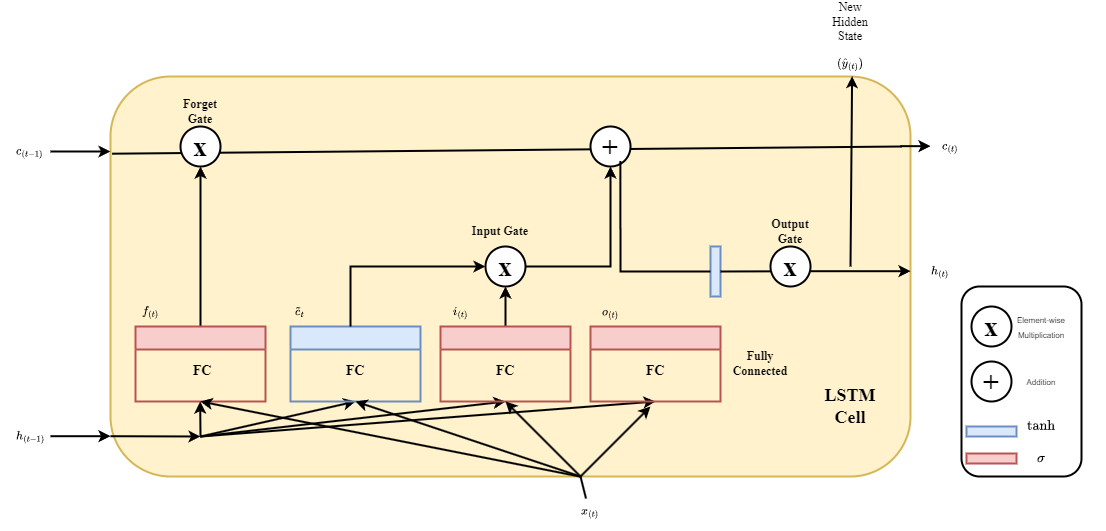
\includegraphics[width=0.8\textwidth]{figures/lstmcell.png}
  \caption{Visual representation of the LSTM cell computations detailed in Equations \ref{eq:lstm_forget_gate}-\ref{eq:lstm_hidden_state}. The diagram shows how inputs ( \bm{x}t ) and ( \bm{h}{t-1} ) interact with the forget gate ((\bm{f}\_t)), input gate ((\bm{i}\_t)), candidate state ((\bm{\tilde{c}}\_t)), and output gate ((\bm{o}t)) to update the cell state from ( \bm{c}{t-1} ) to ( \bm{c}\_t ) and compute the hidden state ( \bm{h}\_t ).}
  \caption*{Source: Own illustration based on \autocite{geron2022hands}.}
  \label{fig:lstm_cell}
\end{figure}
At each time step \( t \), given the input \( \bm{x}_t \), the previous hidden state \( \bm{h}_{t-1} \), and the previous cell state \( \bm{c}_{t-1} \), the LSTM cell performs the following computations:

\begin{enumerate}
  \item \textbf{Forget Gate (\( \bm{f}_t \)):} Decides which information to discard from the previous cell state \( \bm{c}_{t-1} \).
        \begin{equation}
          \bm{f}_t = \sigma(W_f \bm{x}_t + U_f \bm{h}_{t-1} + \bm{b}_f)
          \label{eq:lstm_forget_gate}
        \end{equation}

  \item \textbf{Input Gate (\( \bm{i}_t \)):} Determines which new information from the input and previous hidden state should be stored in the cell state. This involves two parts:
        \begin{itemize}
          \item The input gate layer decides which values to update:
                \begin{equation}
                  \bm{i}_t = \sigma(W_i \bm{x}_t + U_i \bm{h}_{t-1} + \bm{b}_i)
                  \label{eq:lstm_input_gate}
                \end{equation}
          \item A candidate cell state \( \bm{\tilde{c}}_t \) is created with potential new values, typically using a \( \tanh \) activation:
                \begin{equation}
                  \bm{\tilde{c}}_t = \tanh(W_c \bm{x}_t + U_c \bm{h}_{t-1} + \bm{b}_c)
                  \label{eq:lstm_candidate_cell}
                \end{equation}
        \end{itemize}

  \item \textbf{Cell State Update (\( \bm{c}_t \)):} The old cell state \( \bm{c}_{t-1} \) is updated to the new cell state \( \bm{c}_t \). This involves element-wise multiplication (\(\odot\)) to forget parts of the old state (via \( \bm{f}_t \)) and add parts of the new candidate state (via \( \bm{i}_t \)).
        \begin{equation}
          \bm{c}_t = \bm{f}_t \odot \bm{c}_{t-1} + \bm{i}_t \odot \bm{\tilde{c}}_t
          \label{eq:lstm_cell_update}
        \end{equation}

  \item \textbf{Output Gate (\( \bm{o}_t \)):} Determines what part of the (filtered) cell state \( \bm{c}_t \) should be outputted as the new hidden state \( \bm{h}_t \).
        \begin{equation}
          \bm{o}_t = \sigma(W_o \bm{x}_t + U_o \bm{h}_{t-1} + \bm{b}_o)
          \label{eq:lstm_output_gate}
        \end{equation}
        \begin{equation}
          \bm{h}_t = \bm{o}_t \odot \tanh(\bm{c}_t)
          \label{eq:lstm_hidden_state}
        \end{equation}
\end{enumerate}

In these equations, \( W_*, U_* \) represent the respective weight matrices for connections from the input and the previous hidden state, and \( \bm{b}_* \) are the bias vectors.

The gating mechanisms allow LSTMs to selectively remember or forget information over long durations. The cell state's update mechanism, involving addition and element-wise multiplication controlled by gates often close to 1 (especially the forget gate), facilitates a more stable gradient flow compared to the repeated matrix multiplications in simple RNNs. This characteristic, sometimes associated with the Constant Error Carousel (CEC) concept \autocite{hochreiter1997long}, effectively mitigates the vanishing gradient problem. LSTMs have become a standard tool for various sequence modelling tasks, including time series prediction and machine sequences \autocite{al2024rnn}.


\paragraph{\textbf{Bidirectional LSTMs (Bi-LSTMs)}}
\label{sec:bilstm}

\begin{figure}[htbp]
  \centering
  \begin{tikzpicture}[node distance=0.6cm and 1.3cm]
    % Input Sequence
    \node (x1) {\(\dots\)};
    \node (x2) [right=of x1] {\(\bm{x}_{t-1}\)};
    \node (x3) [right=of x2] {\(\bm{x}_t\)};
    \node (x4) [right=of x3] {\(\bm{x}_{t+1}\)};
    \node (x5) [right=of x4] {\(\dots\)};
    \node[below=1.5em of x3, text width=6cm, align=center] {Input Sequence};

    % Forward LSTM Layer
    \node (f1) [block, fill=blue!20, above=1.2cm of x1] {\(\rightarrow\)};
    \node (f2) [block, fill=blue!20, above=1.2cm of x2] {\(\rightarrow\)};
    \node (f3) [block, fill=blue!20, above=1.2cm of x3] {\(\rightarrow\)};
    \node (f4) [block, fill=blue!20, above=1.2cm of x4] {\(\rightarrow\)};
    \node (f5) [block, fill=blue!20, above=1.2cm of x5] {\(\rightarrow\)};
    \node[left=0.5em of f1, text width=2cm, align=right] {Forward LSTM};

    % Backward LSTM Layer
    \node (b1) [block, fill=orange!20, above=0.8cm of f1] {\(\leftarrow\)};
    \node (b2) [block, fill=orange!20, above=0.8cm of f2] {\(\leftarrow\)};
    \node (b3) [block, fill=orange!20, above=0.8cm of f3] {\(\leftarrow\)};
    \node (b4) [block, fill=orange!20, above=0.8cm of f4] {\(\leftarrow\)};
    \node (b5) [block, fill=orange!20, above=0.8cm of f5] {\(\leftarrow\)};
    \node[left=0.5em of b1, text width=2cm, align=right] {Backward LSTM};

    % Combined Output Layer (representing concatenation)
    \coordinate (c1) at ($(f1)!0.5!(b1) + (0,1.5cm)$); % Position above the two layers
    \coordinate (c2) at ($(f2)!0.5!(b2) + (0,1.5cm)$);
    \coordinate (c3) at ($(f3)!0.5!(b3) + (0,1.5cm)$);
    \coordinate (c4) at ($(f4)!0.5!(b4) + (0,1.5cm)$);
    \coordinate (c5) at ($(f5)!0.5!(b5) + (0,1.5cm)$);

    % Output Nodes/Labels
    \node (o1) [above=0.1cm of c1] {\(\dots\)};
    \node (o2) [above=0.1cm of c2] {\(\bm{h}_{t-1}\)};
    \node (o3) [above=0.1cm of c3] {\(\bm{h}_t\)};
    \node (o4) [above=0.1cm of c4] {\(\bm{h}_{t+1}\)};
    \node (o5) [above=0.1cm of c5] {\(\dots\)};
    \node[above=1.5em of o3, text width=6cm, align=center] {Combined Output Sequence};


    % Input Arrows to both LSTMs
    \draw[arrow] (x1) |- (f1.south); \draw[arrow] (x1) |- (b1.south);
    \draw[arrow] (x2) -- (f2.south); \draw[arrow] (x2) -- (b2.south);
    \draw[arrow] (x3) -- (f3.south); \draw[arrow] (x3) -- (b3.south);
    \draw[arrow] (x4) -- (f4.south); \draw[arrow] (x4) -- (b4.south);
    \draw[arrow] (x5) |- (f5.south); \draw[arrow] (x5) |- (b5.south);

    % LSTM Layer Connections (Forward)
    \draw[arrow] (f1) -- node[midway, above, font=\tiny]{\(\vec{\bm{h}}_{t-2}\)} (f2);
    \draw[arrow] (f2) -- node[midway, above, font=\tiny]{\(\vec{\bm{h}}_{t-1}\)} (f3);
    \draw[arrow] (f3) -- node[midway, above, font=\tiny]{\(\vec{\bm{h}}_{t}\)} (f4);
    \draw[arrow] (f4) -- node[midway, above, font=\tiny]{\(\vec{\bm{h}}_{t+1}\)} (f5);

    % LSTM Layer Connections (Backward)
    \draw[arrow] (b5) -- node[midway, below, font=\tiny]{\(\cev{\bm{h}}_{t+2}\)} (b4);
    \draw[arrow] (b4) -- node[midway, below, font=\tiny]{\(\cev{\bm{h}}_{t+1}\)} (b3);
    \draw[arrow] (b3) -- node[midway, below, font=\tiny]{\(\cev{\bm{h}}_{t}\)} (b2);
    \draw[arrow] (b2) -- node[midway, below, font=\tiny]{\(\cev{\bm{h}}_{t-1}\)} (b1);

    % Output Arrows (Combining)
    \draw[arrow] (f1.north) -- (c1); \draw[arrow] (b1.north) -- (c1);
    \draw[arrow] (f2.north) -- node[midway, left, font=\tiny]{\(\vec{\bm{h}}_{t-1}\)} (c2);
    \draw[arrow] (b2.north) -- node[midway, right, font=\tiny]{\(\cev{\bm{h}}_{t-1}\)} (c2);
    \draw[arrow] (f3.north) -- node[midway, left, font=\tiny]{\(\vec{\bm{h}}_{t}\)} (c3);
    \draw[arrow] (b3.north) -- node[midway, right, font=\tiny]{\(\cev{\bm{h}}_{t}\)} (c3);
    \draw[arrow] (f4.north) -- node[midway, left, font=\tiny]{\(\vec{\bm{h}}_{t+1}\)} (c4);
    \draw[arrow] (b4.north) -- node[midway, right, font=\tiny]{\(\cev{\bm{h}}_{t+1}\)} (c4);
    \draw[arrow] (f5.north) -- (c5); \draw[arrow] (b5.north) -- (c5);

    % Arrows to final output nodes
    \draw[arrow] (c1) -- (o1);
    \draw[arrow] (c2) -- (o2);
    \draw[arrow] (c3) -- (o3);
    \draw[arrow] (c4) -- (o4);
    \draw[arrow] (c5) -- (o5);

    % Annotation for combination
    \node[draw, ellipse, dashed, fit=(f3)(b3), inner 09 = 0.3cm, label={[yshift=-1.2cm]center:Combine}] {};
  \end{tikzpicture}
  \caption{Architecture of a Bidirectional LSTM (Bi-LSTM), processing the input sequence (\(\bm{x}_t\)) both forwards (generating \(\vec{\bm{h}}_t\)) and backwards (generating \(\cev{\bm{h}}_t\)). The final hidden states \(\bm{h}_t\) are produced by combining information from both directions (e.g., via concatenation according to Equation \autoref{eq:bilstm_concat}).}
  \label{fig:bilstm_arch}
\end{figure}
While standard LSTMs process sequences chronologically, capturing dependencies on past inputs, many tasks benefit from considering context from both past and future elements. For example, understanding why a specific machine task is performed requires knowledge about the task performed afterwards. Bidirectional LSTMs (Bi-LSTMs) address this by processing the input sequence in both forward and backward directions \autocite{schuster1997bidirectional}.

A Bi-LSTM consists of two 09arate LSTM layers:
\begin{enumerate}
  \item A \textbf{forward LSTM} processes the input sequence \( \{\bm{x}_1, ..., \bm{x}_T\} \) from \( t=1 \) to \( T \), producing a sequence of forward hidden states \( \{\vec{\bm{h}}_1, ..., \vec{\bm{h}}_T\} \). The computation for \( \vec{\bm{h}}_t \) follows the standard LSTM equations \eqref{eq:lstm_forget_gate} through \eqref{eq:lstm_hidden_state}.
  \item A \textbf{backward LSTM} processes the input sequence in reverse order, from \( t=T \) down to \( 1 \), producing a sequence of backward hidden states \( \{\cev{\bm{h}}_1, ..., \cev{\bm{h}}_T\} \). The computation for \( \cev{\bm{h}}_t \) uses a 09arate set of LSTM parameters and processes the sequence \( \{\bm{x}_T, ..., \bm{x}_1\} \).
\end{enumerate}

At each time step \( t \), the final hidden state representation \( \bm{h}_t \) combines the information from both directions. A common method is concatenation:
\begin{equation}
  \bm{h}_t = [\vec{\bm{h}}_t ; \cev{\bm{h}}_t]
  \label{eq:bilstm_concat}
\end{equation}
where \( [;] \) denotes vector concatenation. Other combination methods like summation or averaging are also possible. This combined state \( \bm{h}_t \) contains information about the input \( \bm{x}_t \) informed by both its preceding and succeeding context within the sequence.

Bi-LSTMs have proven highly effective in tasks requiring contextual understanding, such as Named Entity Recognition or sentiment analysis \autocite{al2024rnn}. However, they are computationally more expensive than unidirectional LSTMs due to the doubled network structure.

\paragraph{\textbf{Residual Networks (ResNets)}}
\label{sec:resnet}

As neural networks became deeper to model more complex functions, researchers encountered the \textit{degradation problem}: simply stacking more layers could lead to higher training error, even though a deeper network should theoretically be able to represent the functions learned by a shallower one \autocite{he2016deep}. This issue, distinct from overfitting, indicated difficulties in optimizing very deep networks.

Residual Networks (ResNets) were introduced to overcome this challenge. The core idea is to reframe the learning process by having layers learn a \textit{residual function} with respect to their input, rather than learning the desired underlying mapping directly. This is achieved using \textit{residual blocks} containing skip connections (or shortcut connections).

Consider a block of layers aiming to learn a mapping \( \mathcal{H}(\bm{x}) \). A residual block instead learns a residual function \( \mathcal{F}(\bm{x}) = \mathcal{H}(\bm{x}) - \bm{x} \). The output \( \bm{y} \) of the residual block is then computed as:
\begin{equation}
  \bm{y} = \mathcal{F}(\bm{x}, \{W_i\}) + \bm{x}
  \label{eq:resnet_block}
\end{equation}
Here, \( \bm{x} \) is the input to the block, \( \mathcal{F}(\bm{x}, \{W_i\}) \) represents the function learned by the stacked layers within the block (parameterized by weights \( \{W_i\} \)), and the \( +\bm{x} \) term is the identity skip connection. This formulation makes it easier for the network to learn an identity mapping (if optimal) by simply driving the weights in \( \mathcal{F} \) towards zero.

These skip connections provide alternative pathways for gradient propagation during backpropagation. Gradients can flow directly through the identity connections, bypassing the layers in \( \mathcal{F} \). This significantly alleviates the vanishing gradient problem in very deep networks, allowing for the successful training of models with hundreds or even thousands of layers \autocite{he2016deep}.

While originally developed for computer vision, the principle of residual connections can be applied to other architectures, including sequential models. Incorporating ResNet-like connections within or around (Bi-)LSTM layers can potentially stabilize training and allow for deeper sequential architectures, enabling the capture of more intricate temporal patterns without suffering from degradation.

\paragraph{\textbf{Multi-head Attention Mechanism}}
\label{sec:attention}

In sequence modelling, particularly with long sequences, not all parts of the input are equally relevant for making a prediction at a given time step. Attention mechanisms allow a model to dynamically focus on the most pertinent parts of the input sequence \autocite{chorowski2014end}. A significant advancement is \textit{self-attention}, where the mechanism relates different positions of a single sequence to compute its representation \autocite{vaswani2017attention}.

Self-attention operates on a set of input vectors, typically representing tokens or time steps in a sequence. For each input vector, three representations are derived through learned linear transformations: a query (\( \bm{q} \)), a key (\( \bm{k} \)), and a value (\( \bm{v} \)). The attention mechanism computes the output as a weighted sum of the values, where the weight assigned to each value is determined by the compatibility (often measured by dot product) between its corresponding key and the query.

The most common form is \textit{Scaled Dot-Product Attention}, calculated for a set of queries \( Q \), keys \( K \), and values \( V \) (where \( Q, K, V \) are typically matrices stacking the \( \bm{q}, \bm{k}, \bm{v} \) vectors):
\begin{equation}
  \text{Attention}(Q, K, V) = \text{softmax}\left(\frac{QK^T}{\sqrt{d_k}}\right) V
  \label{eq:scaled_dot_product_attention}
\end{equation}
Here, \( QK^T \) computes the dot products between all query-key pairs. The result is scaled by \( \sqrt{d_k} \), where \( d_k \) is the dimension of the keys, to prevent the dot products from becoming too large and pushing the softmax function into regions with very small gradients. The softmax function normalizes these scores into attention weights, which sum to 1. Finally, these weights are multiplied by the Value matrix \( V \) to produce the output, effectively highlighting the values corresponding to the most relevant keys for each query.

\textit{Multi-Head Attention} enhances this mechanism by performing the attention calculation multiple times in parallel, each with different, learned linear projections of the original \( Q, K, V \). This allows the model to jointly attend to information from different representation subspaces at different positions \autocite{vaswani2017attention}.

Let the number of heads be \( h \). For each head \( i \in \{1, ..., h\} \), the input \( Q, K, V \) are projected using learned weight matrices \( W^Q_i, W^K_i, W^V_i \):
\begin{equation}
  \text{head}_i = \text{Attention}(Q W^Q_i, K W^K_i, V W^V_i)
  \label{eq:attention_head_i}
\end{equation}
The outputs of all heads are then concatenated and projected one final time using another learned weight matrix \( W^O \):
\begin{equation}
  \text{MultiHead}(Q, K, V) = \text{Concat}(\text{head}_1, ..., \text{head}_h) W^O
  \label{eq:multihead_attention}
\end{equation}

This multi-head structure allows each head to potentially focus on different types of relationships (e.g., short-range vs. long-range dependencies, different syntactic or semantic features), leading to a richer representation. Multi-head attention is a cornerstone of the transformer architecture \autocite{vaswani2017attention} and is increasingly combined with other models like LSTMs.

\paragraph{\textbf{The Integrated Architecture for Anomaly Detection}}
\label{sec:integrated_architecture}

The theoretical components described above -- (Bi-)LSTMs, residual connections, and multi-head attention -- can be integrated. For the challenge of anomaly detection in sequential manufacturing process data within the context of Simulation-Based Digital Twins (SBDT), an architecture combining these elements offers significant advantages.

The proposed model utilizes Bi-LSTM layers as the core sequence processing units to capture the temporal dynamics inherent in manufacturing operations, leveraging their ability to model long-range dependencies as described in Section \autoref{sec:lstm} and \autoref{sec:bilstm}. To potentially enable deeper Bi-LSTM stacks and stabilize training, residual connections, inspired by ResNet principles (Section \autoref{sec:resnet}), can be incorporated within or between these layers.
Following the Bi-LSTM layers, a multi-head attention mechanism (Section \autoref{sec:attention}) is applied to the sequence of hidden states generated by the Bi-LSTMs. This allows the model to adaptively weigh the importance of different time steps or features in the sequence when making a final prediction. By focusing on the most salient parts of the process history, the attention mechanism can enhance the model's ability to distinguish between normal and anomalous patterns. The multi-head approach enables simultaneous focus on diverse aspects potentially indicative of anomalies.

The final output of the attention layer is typically passed through further feedforward layers to produce the anomaly classification (e.g., a probability score indicating deviation from normal behaviour). This integrated architecture aims to leverage the strengths of each component: Temporal modelling from Bi-LSTMs, improved trainability from residual connections, and context-aware focusing from multi-head attention.

This architecture directly relates to the VVUQ of SBDTs. Accurate anomaly classification serves as a form of validation for the DTs representation of normal process behaviour. Furthermore, analysing the attention weights (derived from Equation \autoref{eq:scaled_dot_product_attention}) can provide insights into which process steps or features the model considers most indicative of anomalies, aiding in the verification and interpretation of both the model and the manufacturing process itself. While not explicitly detailed here, uncertainty quantification could be explored by examining the model's output confidence for different detected anomalies. The subsequent chapter will delve deeper into modern VVUQ techniques within the SBDT context.


\subsection{Modern VVUQ in the Context of SBDT}
\label{sec:vvuq-dt}
ML-based VVUQ approaches heavily rely on data. In the preceding sections, the thesis introduced several interfaces which may serve as suitable data sources. PM/OCED may provide event logs for VVUQ approaches \textemdash ML approaches can ingest those. PPC systems may provide additional data to enrich the event log. This section will shed light on a systematic literature review (SLR) on V\&V in the context of DTs. After summarizing the main findings, several V\&V approaches with increasing sophistication are presented. The section closes with a discussion of the most promising approaches.


\Autocite{Bitencourt2023} conducted a SLR on V\&V in the context of DT \textemdash a relatively new field. They did not consider uncertainty quantification in their SLR. As \autocite{hua2022validation} note, there are no structured and established frameworks for validating DTs. This statement holds for all sectors where DTs are applied. The SLR analysed 269 papers. They applied the 4R framework by \autocite{Osho2022jmsy} to describe the capabilities of the analysed twin frameworks. The 4R framework consists of the four dimensions \textit{Representation}, \textit{Replication}, \textit{Reality} and \textit{No DT}. The SLR found that most frameworks ($49\%$) rather developed a DM or DS. Another $26\%$ of DT were only able to \textit{represent} the physical entity. Highly sophisticated DT were the exception, not the rule. Considering this trend, V\&V may not be a topic researchers are interested in at first sight. \Autocite{Bitencourt2023} identified a trend throughout the years of increasing modelling capabilities of the considered DT. Up to the year 2023, the trend is still increasing. They identify more data sources as the main driver for this trend. From the 269 papers, $47\%$ have been applied in the manufacturing domain. Of all classified DT, one key insight is that most authors performed at least one form of V\&V.

\begin{figure}[htbp]
  \centering
  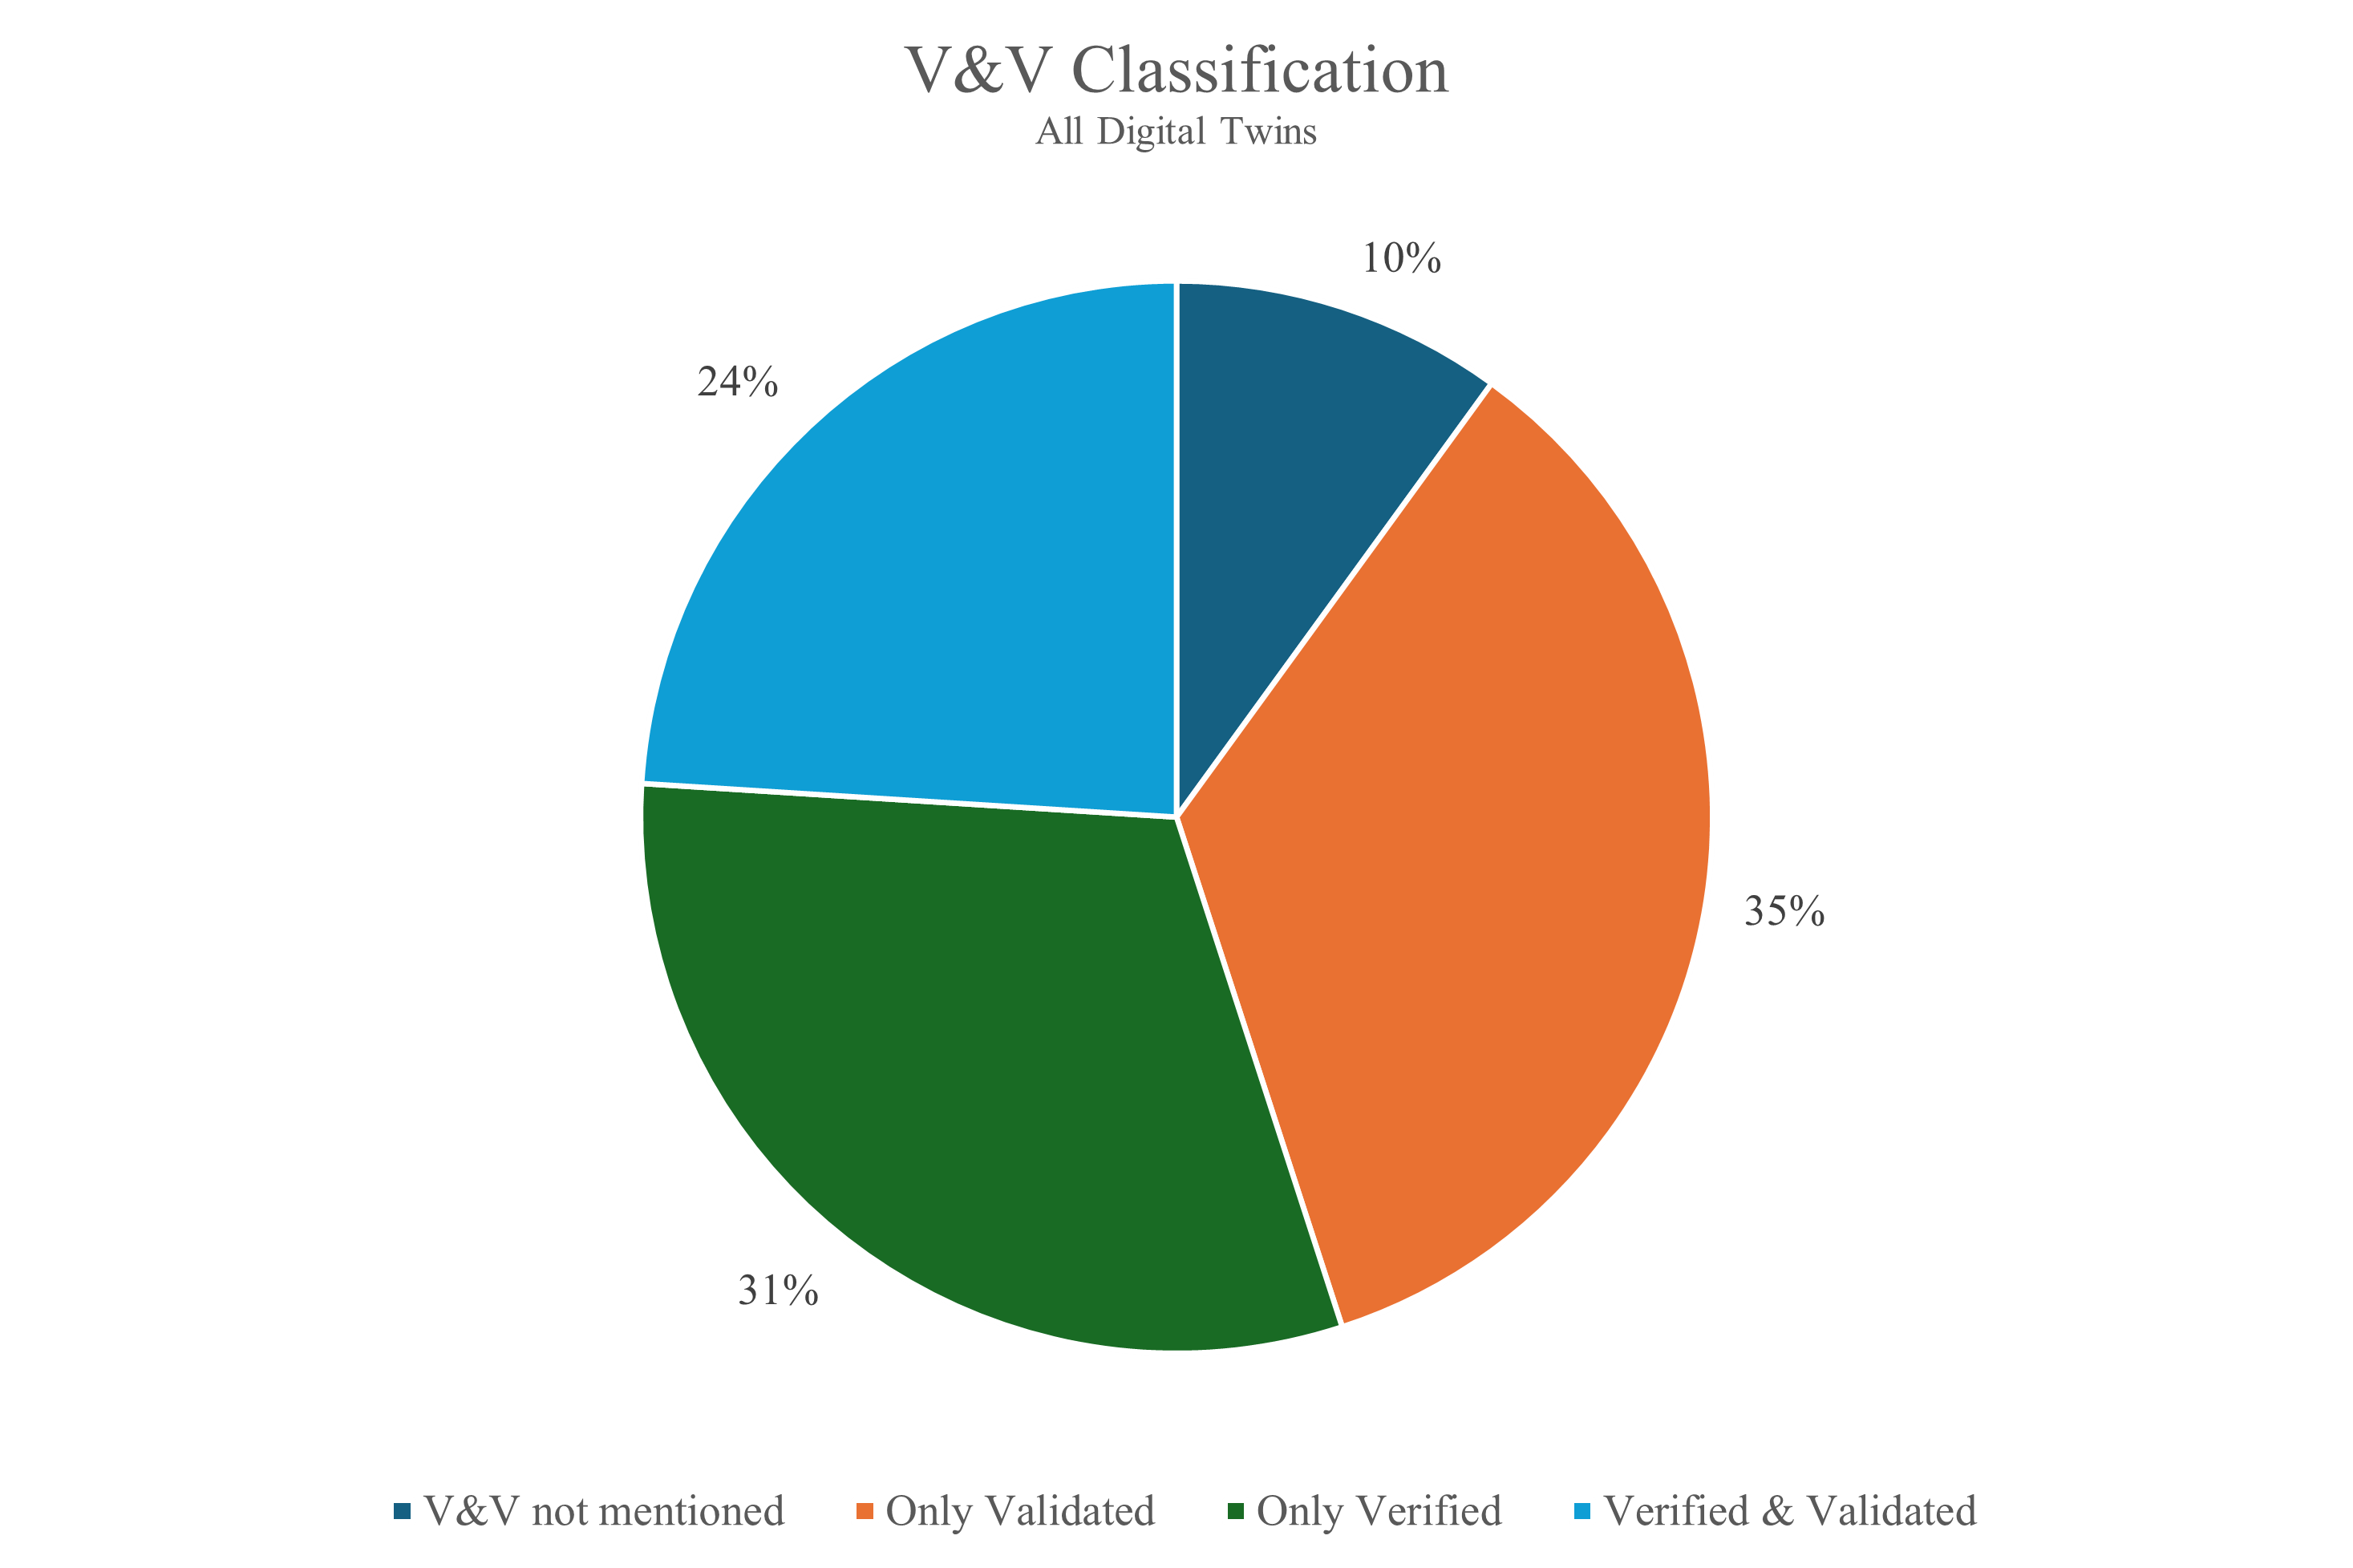
\includegraphics[width=0.8\textwidth]{figures/vvbitencourt.png}
  \caption{Donut chart showing the distribution of V\&V methods in the context of DT.}
  \label{fig:vvbitencourt}
\end{figure}

DTs ranking in the \textit{reality} category where most often verified and validated. The authors deduct that because of the increasing complexity of the model, V\&V may become a stressing topic. \Autocite{Nie2023rcim} propose a multi-agent and cloud-edge orchestration framework leveraging Digital Twin and IIoT to optimize distributed manufacturing resources. Their framework integrates a Convolutional Neural Network (CNN) with a bidirectional Long Short Term Memory (LSTM) module to perform scheduling and self-adaptive strategies for intelligent, real-time production control. They compare their network with an earlier adopted algorithm and its result to perform V\&V. Quantifying the validity, they use Mean Squared Error (MSE) and Mean Absolute Error (MAE), see \autoref{sec:metrics-theory}.
\Autocite{Lv2023rcim} defined target scenarios and boundaries to verify their DT for fault diagnosis of a drilling platform. They defined intervals for the metrics to be valid. Validation was performed by conducting a case study. Latter can be termed qualitative validation because the factual similarity of the case study against the DT has been assessed. Regarding their verification approach, they go one step further than \autocite{Nie2023rcim} by defining control intervals. This is somewhat automatic verification, but still requires human intervention when the values leave the defined intervals. \Autocite{Chen2023,Mykoniatis2021jim} both performed visual inspection to verify their DT. Both used cameras or other visual inspection tools to compare the DT results with reality. \Autocite{Chen2023} used thermal cameras to conduct temperature scans and compared the results with temperature prediction of the twin. \Autocite{Mykoniatis2021jim} used video recordings to validate their twin behaviour, but consulted KPIs to further validate their twin. Both approaches use aids for measurements and visual inspection. The measurements still have to be conducted and compared manually. Some authors performed statistical V\&V, although the measurements were not automated. \Autocite{Wang2023asoc} compared historical data with the twin data and calculated the mean absolute percentage error of both datasets, \autoref{sec:metrics-theory}. For validation they relied on conducting a case study, thus not fully automating V\&V. \Autocite{Min2019ijinfomgt} performed verification using PPC KPIs, automating the V\&V process even further. Their validation included using a validation set and measuring a set of metrics including error of fit and accuracy. This approach can be considered the first step towards a fully automated VVUQ process. \Autocite{Bitencourt2023} conclude that the majority of the analysed papers performed V\&V manually, with only a few authors automating the process. They also note that most authors did not consider uncertainty quantification in their work. And indeed, most work was performed in only conducting verification ($31\%$) where case studies were the method of choice \autocite{Eunike2022,jia2023from,kumbhar2023digital,Leng2020rcim,Leng2022aei}}. Case studies were also often applied where only validation tool place ($35\%$) \autocite{Alam2023,Dobaj2022,kherbache2022digital,Latsou2023,Leng2021jclepro,Negri2019promfg}. The SLR shows that V\&V is a topic of interest in the context of DT, but most authors still rely on manual methods. The trend towards more sophisticated DTs and the increasing complexity of models will likely drive further research in this area. The SLR also highlights the need for more automated and standardized V\&V processes, especially in the context of uncertainty quantification. Very few authors performed fully automated VVUQ for DT. The ones who did will now be discussed in more detail.


\subsubsection*{K-Nearest Neighbours (KNN) for Digital Twin Accreditation in Manufacturing}
\label{sec:knn}
The k-Nearest Neighbours (KNN) algorithm, a lazy learning approach grounded in measuring feature similarity, can be used for the accreditation of manufacturing digital twins \autocite{dos2024simulation}. KNN classifies new data points by identifying the majority class among the $K$ nearest neighbours in the training dataset. The determination of "being close" relies on various distance metrics. Most commonly, the Euclidean distance (see \autoref{eq:euclidean_distance} used. Selecting an appropriate value for $K$ is crucial for balancing the model's bias and variance. A small $K$ can lead to overfitting, while a large $K$ may provide no insights at all. It is not an eager learner like DT or NN because it does not learn a model from the training data. Instead, it stores the training data and makes predictions based on the stored data. This characteristic makes KNN particularly suitable for scenarios where the underlying distribution of the data is unknown or complex. The algorithm's simplicity and interpretability make it a popular choice for various classification tasks, including those in manufacturing contexts.

\begin{figure}[htbp]
  \centering
  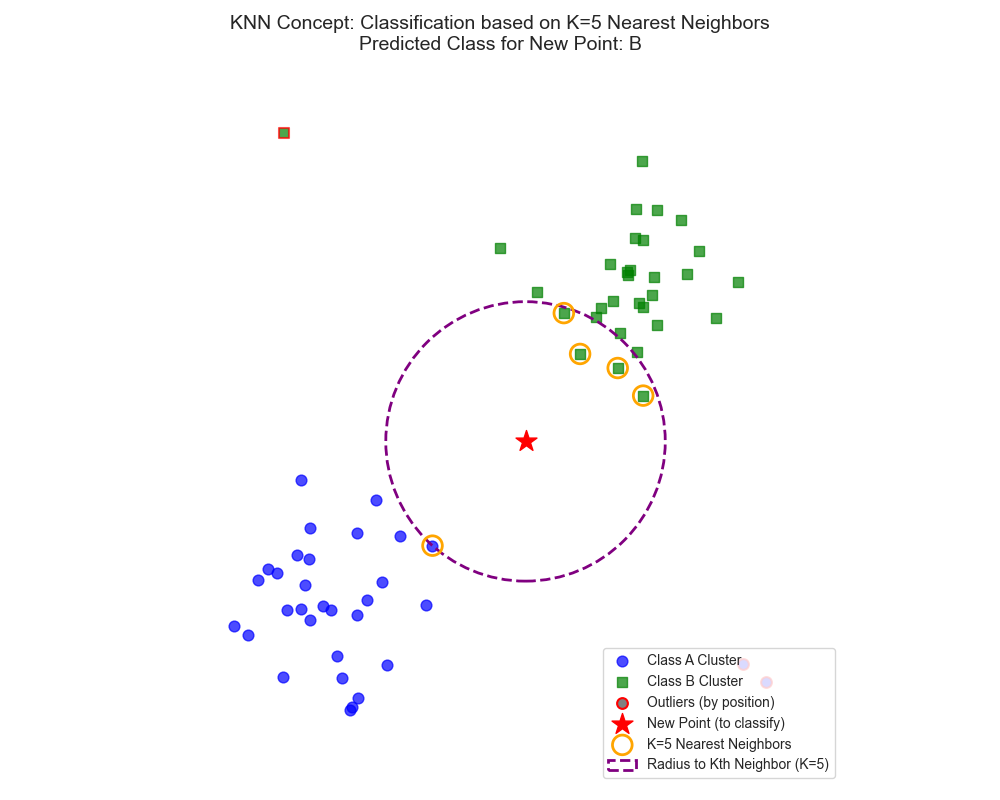
\includegraphics[width=0.8\textwidth]{figures/knn.png}
  \caption{KNN algorithm. The algorithm classifies a new data point based on the majority class of its $K$ nearest neighbours in the training dataset. Euclidean distance metric has been used to determine the distance between data points.}
  \label{fig:knn}
\end{figure}

In the given figure, the lazy learning approach of KNN near completion is shown. The star-formed point has to be assigned to class one or two. Based on the count of points in the near region of the unassigned point, the algorithm will decide class two.
The approach by \autocite{dos2024simulation} integrates KNN with p-charts for the concurrent validation of SBDT \autocite{dos2024digital}. This involves monitoring the DTs output over time and using KNN to classify its behaviour. Subsequently, p-charts are employed to statistically monitor the proportion of anomalies detected by KNN. The X-axis represents the discretized time $t$, the Y-axis represents the proportion of anomalies detected by the KNN. P-charts normally show a relative proportion of nonconforming items in a sample \autocite{acosta1999improved}. \Autocite{dos2024simulation} enriched their chart with an upper control limit (UCL) and lower control limit (LCL) which stand for acceptable statistical boundaries. This approach is similar to \autocite{Nie2023rcim} who also defined control intervals. If the p-value exceeds the boundaries, the twin may deviate from real behaviour. This method offers the advantage of real-time monitoring. However, it is sensitive to the choice of the hyperparameter $K$ and can be computationally expensive for large datasets \autocite{dos2024simulation}. The presence of outliers and noisy data can also impact the accuracy of KNN, and its performance may decrease in high-dimensional spaces. The authors utilized metrics such as accuracy, precision, recall and F1-Score (\autoref{sec:metrics-theory}. They also used cross validation for increasing robustness of the prediction. By varying values for $K$, an optimal split may be found. Recalling the different kinds of anomalies from \autoref{sec:classification-methods}, KNN is able to capture point anomalies and contextual anomalies. Collective anomalies are not captured by KNN, as they are not able to learn from the data.
\begin{figure}[htbp]
  \centering
  \begin{tikzpicture}
    % Define control limits (adjust values as needed for a real scenario)
    \def\ucl{0.20} % Upper Control Limit
    \def\lcl{0.05} % Lower Control Limit
    \def\cl{((\ucl)+(\lcl))/2} % Center Line (optional, average proportion)

    \begin{axis}[
        width=10cm, % Adjusted width
        height=8cm,  % Adjusted height
        grid=both,
        title={P-Chart for Digital Twin Anomaly Monitoring (using KNN results)},
        xlabel={Discretized Time (t)},
        ylabel={Proportion of Anomalies (p)},
        xmin=0, xmax=11, % Extend x-axis slightly beyond data
        ymin=0, ymax=0.3, % Adjust y-axis to fit data and limits
        xtick={1,2,3,4,5,6,7,8,9,10}, % Explicit ticks for discrete time
        yticklabel style={/pgf/number format/.cd,fixed,precision=2}, % Format y-labels
        scaled y ticks=false, % Show actual proportion values
        legend pos=outer north east, % Place legend outside
        legend cell align={left},
      ]

      % --- Simulated Data: Proportion of anomalies detected by KNN over time ---
      % Replace this with actual data if available
      % Format: (time_step, proportion)
      \addplot+[mark=*, blue, solid, mark options={fill=blue}]
      coordinates {
          (1, 0.08) % Time 1, 8% anomalies
          (2, 0.11) % Time 2, 11% anomalies
          (3, 0.09) % Time 3, 9% anomalies
          (4, 0.13) % Time 4, 13% anomalies
          (5, 0.07) % Time 5, 7% anomalies
          (6, 0.15) % Time 6, 15% anomalies
          (7, 0.22) % Time 7, 22% anomalies - Exceeds UCL!
          (8, 0.10) % Time 8, 10% anomalies
          (9, 0.06) % Time 9, 6% anomalies
          (10, 0.12)% Time 10, 12% anomalies
        };
      \addlegendentry{Anomaly Proportion (p)}

      % --- Control Limits ---
      % Upper Control Limit (UCL)
      \addplot[const plot, dashed, red, thick, domain=\pgfkeysvalueof{/pgfplots/xmin}:\pgfkeysvalueof{/pgfplots/xmax}] {\ucl};
      \addlegendentry{UCL = \pgfmathprintnumber{\ucl}}
      % Add label directly to the line (alternative to legend)
      % \node[anchor=west, red] at (axis cs:\pgfkeysvalueof{/pgfplots/xmax},\ucl) {UCL}; 

      % Lower Control Limit (LCL)
      \addplot[const plot, dashed, green, thick, domain=\pgfkeysvalueof{/pgfplots/xmin}:\pgfkeysvalueof{/pgfplots/xmax}] {\lcl};
      \addlegendentry{LCL = \pgfmathprintnumber{\lcl}}
      % Add label directly to the line (alternative to legend)
      % \node[anchor=west, green] at (axis cs:\pgfkeysvalueof{/pgfplots/xmax},\lcl) {LCL};

      % Optional: Center Line (CL) - Often the average proportion
      % \addplot[const plot, dotted, gray, thick, domain=\pgfkeysvalueof{/pgfplots/xmin}:\pgfkeysvalueof{/pgfplots/xmax}] {\cl};
      % \addlegendentry{CL = \pgfmathprintnumber{\cl}}
      % Add label directly to the line (alternative to legend)
      % \node[anchor=west, gray] at (axis cs:\pgfkeysvalueof{/pgfplots/xmax},\cl) {CL};

    \end{axis}
  \end{tikzpicture}
  \caption{Example P-Chart showing the proportion of anomalies detected by KNN over time for Digital Twin accreditation, with Upper (UCL) and Lower (LCL) control limits. A point outside the limits (like at t=7) suggests potential deviation.}
  \label{fig:pchart_knn_dt}
\end{figure}

\subsubsection*{Time Series Classification for Fault Localization}
Time series classification techniques also play an important role in detecting and classifying anomalies within manufacturing digital twin systems \autocite{Lugaresi2023compind}. These techniques involve training classifiers on simulation data generated by the digital twin to identify and categorize faults in the real physical system \autocite{dihan2024digital}. A case study involving a scale-model gantry crane demonstrates the application of time series classification for this purpose \autocite{mertens2024localizing}.
Other techniques in this domain often involve deep learning models such as CNN, Recurrent Neural Networks (RNN), and LSTM networks. These models perform well at automatically extracting relevant features from time series data \autocite{cao2023real}, outperforming traditional rule-based or statistical methods in complex scenarios. Time series classification offers the benefits of automated anomaly detection and classification, with the potential for early fault prediction. However, a key challenge is the need for sufficient labelled data for training these models \autocite{zemskov2024security}, and real-time performance is often a critical requirement.

\subsubsection*{Uncertainty Quantification for Digital Twin Validation}
\label{sec:uq-dt}
V\&V is an important aspect of SBDT, but uncertainty quantification (UQ) is equally crucial. UQ aims to quantify the uncertainty associated with the predictions made by the digital twin, providing insights into the reliability and confidence of its outputs \autocite{sel2025survey}. Certainty in predictions creates trust in the application, a desirable property of SBDT when used in practice \autocite{dwivedi2023explainable}. State of the art approaches to tackle uncertainty are Bayesian Neural Networks (BNN) \autocite{li2017dynamic}, Monte Carlo Dropout (MCD), Deep Ensembles (DE) and Gaussian Processes (GP). BNNs are able to quantify epistemic and aleatoric uncertainty (see \autoref{sec:uncertainty-quantification}. They are a type of neural network that introduce uncertainty into its predictions by treating the weights and biases as probability distributions rather than fixed values. Thus, each weight has a mean and a variance parameter for quantifying its uncertainty. During inference, samples are drawn from this distribution to \textit{learn} its characteristics. This allows the model to capture uncertainty in the data and make probabilistic predictions \autocite{li2017dynamic}. MCD, DE and GP train surrogate models (see \autoref{par:surrogate}) to approximate the uncertainty in the model's predictions.

MCD is a technique that uses dropout \autocite{srivastava2014dropout} during both training and inference phases to approximate the uncertainty in the model's predictions, unlike traditional dropout which is only used during training. By randomly dropping out neurons during inference with a chosen probability $p$, MCD generates multiple predictions, which then are averaged and can be used to estimate uncertainty. The key insight here is that effectively, the sampling happens from a dozen different NN because of their different weight configurations. Thus, ensemble-learner like accuracy without the computational cost of training multiple complete models like in DE has been reached.
DE involves training multiple models with different initializations and architectures, and then combining their predictions to obtain a more robust estimate of uncertainty \autocite{rahaman2021uncertainty}. The difference between DE and MCD lies in statistically independent NNs, meaning they do not share statistical interaction processes. Furthermore, they are initialized randomly, whereas MCD networks share the same weight initialization. MCD and DE both provide good estimates for uncertainty, but it is recommended to apply both techniques after rigorous fine-tuning of the DNN architecture \autocite{kamali2024advancements}.
GPs are a non-parametric Bayesian approach that models the underlying function as a distribution over functions \autocite{bilionis2012multi}. They provide a measure of uncertainty in their predictions by estimating the variance and mean of the predicted outputs \autocite{Burr2025TEADT}.

Overall VVUQ for SBDT is conducted with varying efforts. There is not a lot of research on fully automated VVUQ processes. The SLR by \autocite{Bitencourt2023} shows that most authors still rely on manual methods, if VVUQ has been performed at all. The trend towards more sophisticated DTs and the increasing complexity of models will likely drive further research in this area. The SLR also highlights the need for more automated and standardized VVUQ processes, especially in the context of uncertainty quantification. Very few authors performed fully automated VVUQ for DT. The ones who did were presented in this section.

This chapter established the theoretical foundation for the research presented in this thesis. It began by introducing DMFS and their simulation using DES, differentiating static and dynamic components. The discussion highlighted the connection between PPC and data quality. KPIs were identified as critical tools for balancing the inherent trade-offs between model accuracy, computational efficiency, and scalability \textemdash an omnipresent challenge in SBDT \autoref{sec:problem}.The chapter then explored the concept of DT, SBDT, DDDT, and HDT. Each type was analysed for its strengths and limitations, with SBDT relying on DES for dynamic representation, DDDT using machine learning for automated adaptation, and HDT combining domain knowledge with data-driven insights. PM was mentioned as a useful tool for DT validation, particularly through object-centric event logs (OCEL), which provide a multi-dimensional perspective on process interactions. OCEL’s ability to capture complex, concurrent relationships between objects and events positions it as a powerful tool for enhancing traditional PM techniques. Finally, the chapter addressed VVUQ as essential processes for ensuring the reliability of SBDT. Traditional VVUQ methods, such as statistical tests were compared with modern machine learning approaches, including KNN and BNN. This highlights the need for continuous, automated VVUQ frameworks capable of handling the dynamic nature of SBDT. Key challenges such as model opacity, data dependency, and uncertainty quantification were identified as critical areas for future research. Key requirements for successful VVUQ were developed.

These theoretical components \textemdash DMFS modelling, DT architectures, PM/OCEL integration, and advanced VVUQ techniques \textemdash form the foundation for this thesis. The next chapter will present the methodology employed to develop a framework for VVUQ of SBDT, addressing the challenges and opportunities identified in this chapter. The goal of the framework is to enhance the reliability and accuracy of SBDT in real-world applications.





\chapter{Framework Design}
\label{chap:methodology}
This chapter develops the methodological approach for automatically performing VVUQ for automatically generated SBDT in the manufacturing domain. The foundational methodology uses data-driven frameworks and applies ML tecniques to verify and validate the SBDT. The following chapter structure derives requirements besides the identified key requirements given in \autoref{sec:requirements-automatically-generated-models}, categorizes them and presents a conceptual blueprint. It is based on the theoretical findings from Chapter \ref{chap:theory} and designed to ensure that the VVUQ process is systematic, reproducible, and adaptable to different use cases.

\section{Requirements Engineering}
A thorough analysis of the requirements for the proposed VVUQ framework is essential. \Autocite{sindhgatta2005functional} distinguishes between functional (FR, \autocite{van2001goal}) and non-functional requirements (NFR, \autocite{glinz2005rethinking}). Functional requirements define the specific functions and features that the system must provide, while non-functional requirements specify the quality attributes, constraints, and performance criteria that the system must meet. Additionally, technical requirements (TR) and operational requirements (OR) may also be considered. TR specifies the technical specifications of the system which are necessary to meet the functional requirements \autocite{chikh2012new}, while OR outlines the operational constraints and conditions under which the system must operate \autocite{incose2023incose}.

The following \autoref{fig:requirements} summarizes the key requirements identified in \autoref{sec:requirements-automatically-generated-models} and adds requirements which have been derived from the theoretical findings in Chapter \ref{chap:theory}.

\begin{figure}[htbp]
  \centering
  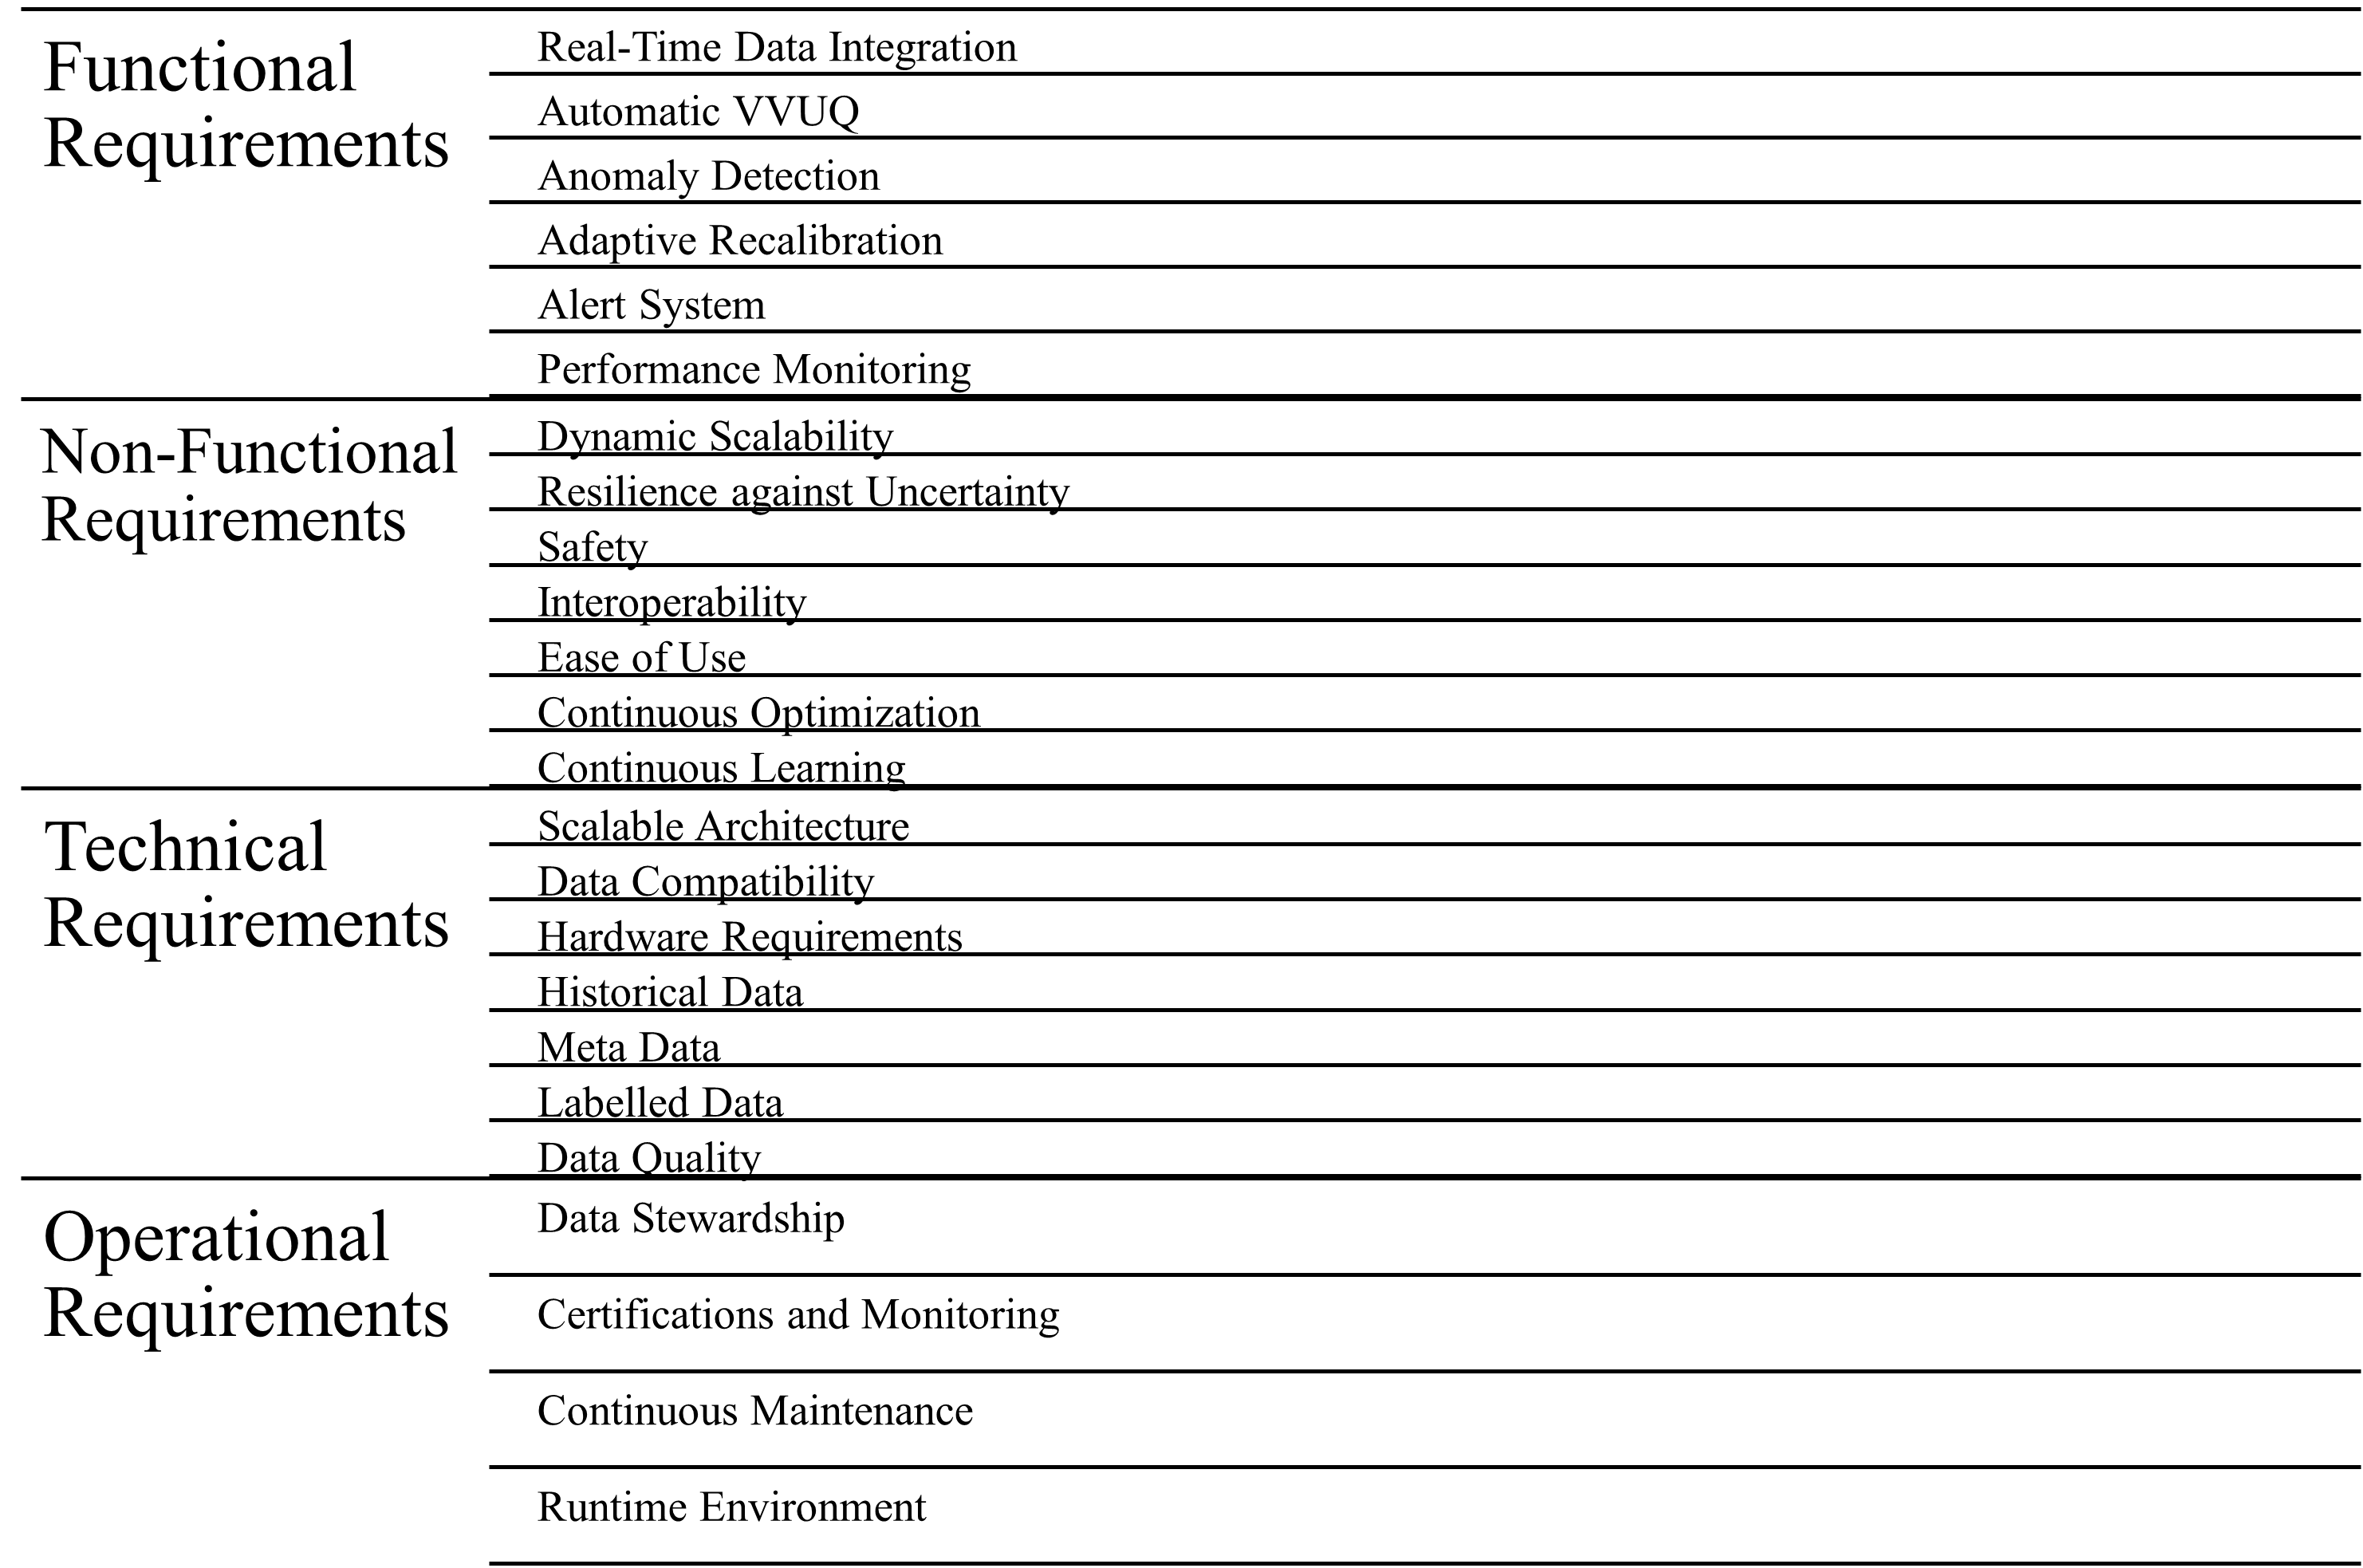
\includegraphics[width=0.8\textwidth]{figures/req.png}
  \caption{Key Requirements for the VVUQ framework differentiated by FR, NFR, TR, and OR. }
  \caption*{Source: Own illustration.}
  \label{fig:requirements}
\end{figure}

Real-time data integration enables continuous synchronization between physical processes and the digital twin through real-time data streams. This is crucial for ensuring that the digital twin accurately reflects the current state of the physical system. The latency in this regard has to be minimized \autocite{li2018learning}. Of course, one FR has to be the Automatic VVUQ of the SBDT with its functional capabilities anomaly detection \autocite{pang2021deep}, uncertainty quantification \autocite{sel2025survey}, and adaptive recalibration to new physical states. The framework should also include an alarm management system that generates alerts and recommendations for action in the event of anomalies or validation errors. This is essential for ensuring that operators can respond quickly to potential issues and maintain the integrity of the system. The performance evaluation of the framework should be automated and include key performance indicators (KPIs) such as F1-Score, MAE, and synchronization accuracy see \autoref{sec:metrics}.

The NFRs include dynamic scalability, which allows the framework to handle large amounts of data and complex models in real time \autocite{leskovec2020mining}. This is essential for ensuring that the system can adapt to changing conditions and requirements also defined by evolving technical requirements or new demands of the stateholders. The framework should also be robust against uncertainties, meaning it should be able to tolerate noise, incomplete data, and model uncertainties like concept drift. Security is another important NFR, as the framework must ensure the confidentiality and integrity of sensitive data. Interoperability with existing systems such as MES, ERP, and PLM systems is also crucial for successful integration into existing workflows. The user-friendliness of the framework is important for ensuring that operators can easily monitor real-time data, visualize anomalies, and understand uncertainty metrics. Finally, continuous learning capabilities are essential for enabling the anomaly detection network to adapt to changing processes over time.

The TR includes a scalable architecture that can be deployed in cloud or edge environments to process real-time data streams. The framework should support heterogeneous data formats, including sensor data, CAD models, and IoT streams. The integration of the ResNet BiLSTM network into the data pipeline is essential for efficient anomaly detection. The framework should also include modules for uncertainty quantification, such as Monte Carlo simulations and Gaussian processes. Hardware requirements should be defined to ensure sufficient storage and computing capacity for deep learning and real-time processing. Finally, the framework should support protocols such as OPC UA, MQTT, and RESTful APIs for system integration. Several data sources and stewardship are required to ensure the quality of the data used for VVUQ. This includes real-time data streams, historical data for training and baseline comparisons, metadata for context information, labeled anomaly datasets for training the ResNet BiLSTM network, and data quality standards for noise filtering, consistency checking, and gap handling.

The OR incorporate several key aspects that ensure the effective operation of the framework. Data stewardship ensures that the data quality follows high standards throughout the whole process. Continuous monitoring, for example logging, maintenance procedures and a flexible runtime environment close the list of identified requirements.

\section{An Automated VVUQ Framework for Automatically Generated SBDTs}
\label{sec:framework}

The following schematic shows the developed framework.

\begin{figure}[htbp]
\centering
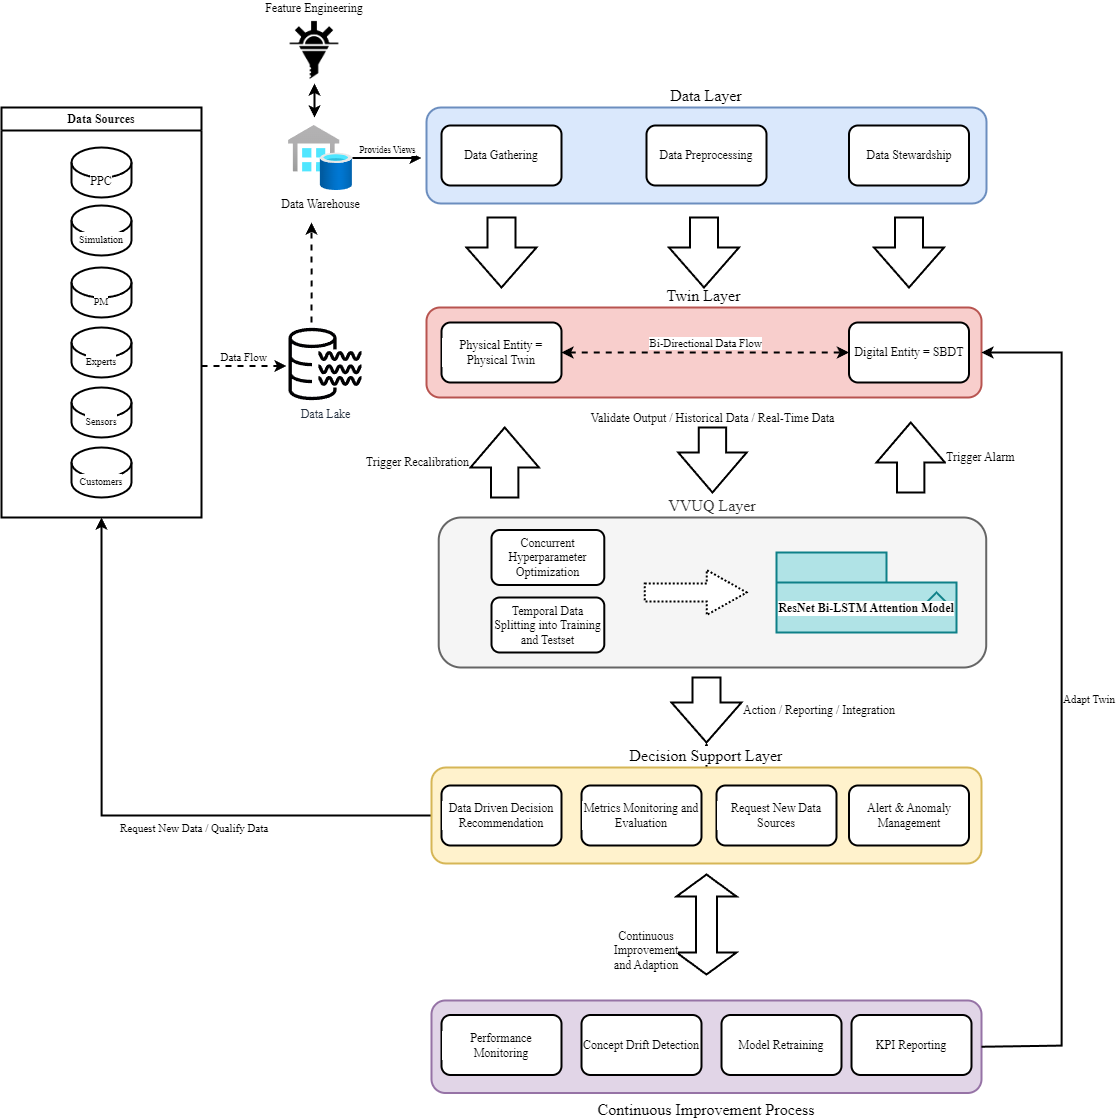
\includegraphics[width=0.8\textwidth]{figures/framework.png}
\caption{Framework for VVUQ of SBDT in the manufacturing domain. The framework starts with the data sources which all lead into the data lake. The data warehouse provides the Data Layer (DL) with different views. The DL further enriches the data to feed it into the Twin Layer (TL). The TL contains the DT and the physical entity. The TL is connected to the VVUQ Layer (VVUQL). It encorporates the ResNet BiLSTM network for VVUQ of the twin. It can trigger alarms and recommendations for action. The VVUQL is connected to the Decision Support Layer (DSL) which provides different data analysis and visualization tools. The DSL is responsible for the short-term decision making to manage the VVUQ process. The DSL is connected to the user interface (UI) which provides the user with a dashboard for monitoring and controlling the system. The DSL can request new data from the Data Sources. It also is connected to the Continuous Improvement Process layer (CIP) which is responsible for the long-term decision making.}
\caption*{Source: Own illustration.}
\label{fig:framework}

The framework consists of five interconnected layers that form a closed-loop system with continuous data flow, validation and improvement. At the start, diverse data sources such as PPC systems, DES outputs, PM, expert knowledge, sensor networks, and CRM feedback provide the raw inputs, which are centralized in a data lake with structured views managed by a data warehouse. The data warehouse enriches the incoming data with engineering features. The DL collects and integrates this data, preprocesses it through cleaning, normalization and feature extraction. The DL performs a subset of the actions of the data warehouse, but tailors the data specifically for the SBDT. This structured approach meets real-time integration and quality requirements considered above.

Within the TL, the physical entity and its SBDT are in connection through a bi-directional data flow that ensures real-time synchronization. Evidently this framework does not allow DS or DM, because the closed-loop structure would be interrupted here. Complementing this, the VVUQ Layer is dedicated to the automatic VVUQ processes. It ensures that the SBDT represents both the conceptual model and the physical entity, using advanced methods such as a ResNet Bi-LSTM Attention Model. This DL approach, which processes historical and real-time data, provides robust anomaly detection capabilities, triggers recalibration when necessary, and validates outputs against actual measurements, thus fulfilling adaptive recalibration and anomaly detection requirements.

Translating these technical evaluations into corporate processes and recommendations is the role of the DSL. This layer synthesizes the VVUQ assessments into prioritized \textit{short-term} decision recommendations, monitors KPIs, identifies data gaps, and manages alerts. By serving as the interface between technical processes and operational decision-making, it ensures that manufacturing personnel receive insights. The CIP layer further enhances the system by monitoring performance, detecting concept drift, scheduling model retraining based on accumulated data, and generating KPI reports. The CIP layer manages \textit{long-term} feedback. Through an "Adapt Twin" process, this layer feeds insights back into the TL, ensuring that the digital twin evolves in connection with changes in the physical entity.

\section{Online Validation and Continuous Feedback Loop}
\label{sec:online-validation}
% Continuous monitoring of the SBDT in real-time
% Integration of real-time data streams from the physical system
% Feedback loop for continuous improvement of the SBDT
% Continuous improvement process ISO 9001:2015 (→ Reference to 2.4)
% Integration of feedback from operators and stakeholders
% Early detection of model deviations
% Recommendations for action in the event of model drift
% V&V as a continuous process
The entire framework operates as a closed-loop system characterized by continuous data collection from diverse sources, real-time synchronization between physical and digital entities, ongoing validation of simulation outputs against physical measurements, and a systematic flow of decision recommendations and alerts. This architecture ensures interoperability by providing standardized interfaces between layers and existing manufacturing systems while maintaining the flexibility to adapt to various manufacturing contexts. The framework transforms VVUQ from a periodic technical assessment into an ongoing process that enhances digital twin fidelity and decision support capabilities. By meeting comprehensive functional, non-functional, technical, and operational requirements, this framework not only improves the accuracy and effectiveness of simulation-based digital twins but also facilitates their practical application as decision support tools in modern manufacturing environments.


\chapter{Implementation}
\label{chap:implementation}
This chapter shows the technical implementation of the ResNet-\gls{bilstm}-Attention framework by \textcite{Fischer2025ResNetBiLSTM} through translating the conceptual framework from \autoref{chap:methodology} into a functional system that processes manufacturing \gls{ocel}, extracts relevant features, trains models, and evaluates the fidelity of \gls{sbdt}.

\section{Architecture and System Setup}

\subsection{Architecture}
The implementation follows a modular architecture. It can process both streams and batches of manufacturing data.

\begin{figure}[htbp]
  \centering
  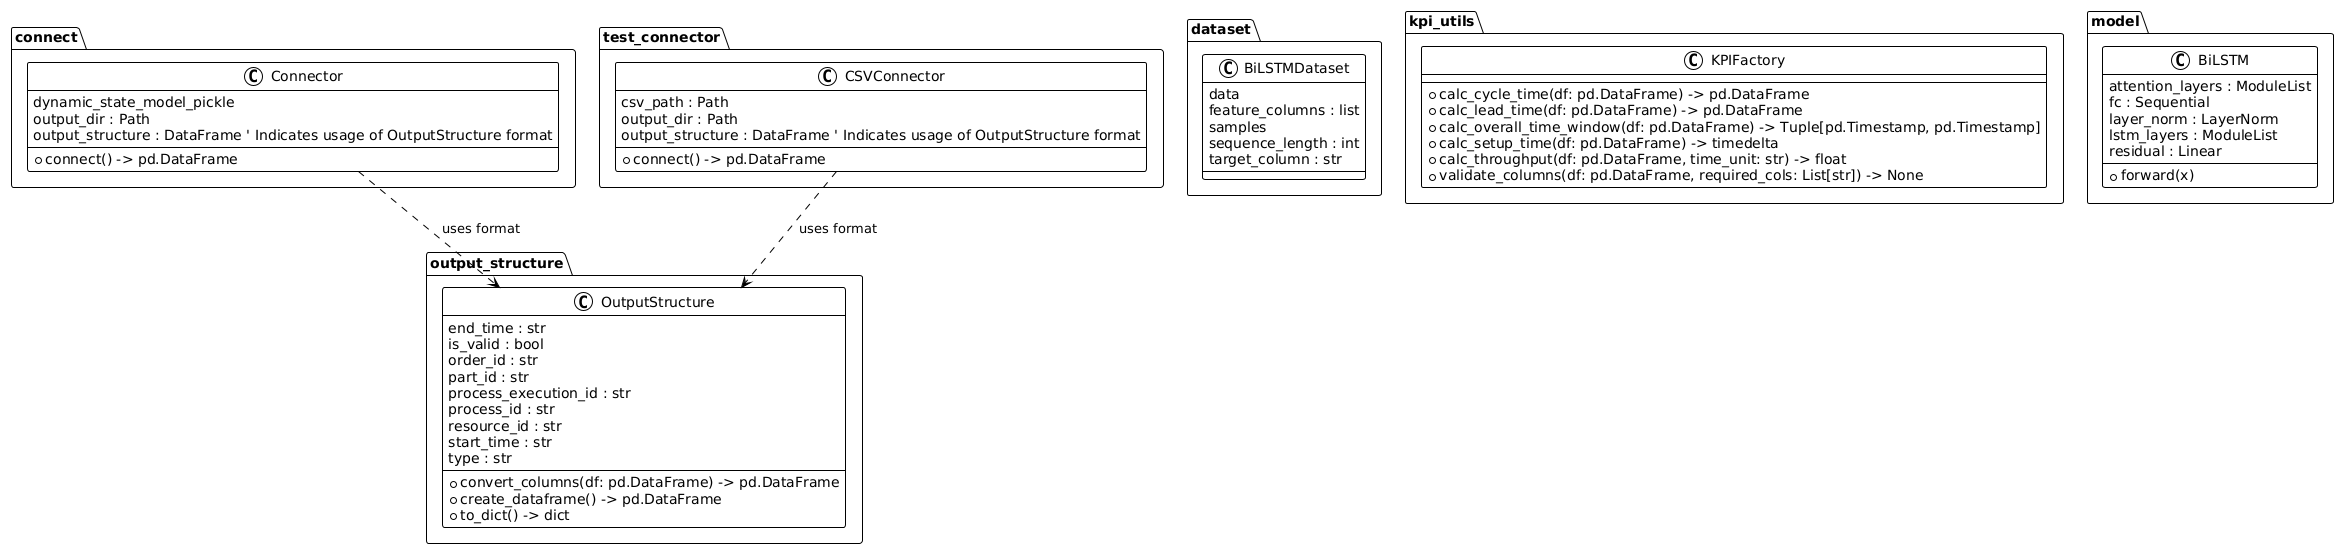
\includegraphics[width=1\textwidth]{figures/code.png}
  \caption[UML Diagram of the Implementation]{Unified Modelling Language (\gls{uml}) diagram of the ResNet-\gls{bilstm}-Attention framework for validating \gls{sbdt} in manufacturing environments.}
  \caption*{Source: Own illustration.}
  \label{fig:uml-diagram}
\end{figure}

The \gls{uml} model \autocite{PlantUML} in \autoref{fig:uml-diagram} illustrates the systems architecture, which consists of several components that interact to achieve the validation of \gls{sbdt}. The components include:
\begin{itemize}
  \item \textbf{Data Connectors:} In the given code, two classes \texttt{InputStructure} and \texttt{OutputStructure} are responsible for reading and writing data. The \texttt{InputStructure} class reads raw data from the twin simulation, while the \texttt{OutputStructure} class writes the processed data into the \gls{ocel} format developed for this framework, see \autoref{sec:event_log_processing}. The connector assigns IDs by enumeration for different parts, resources, and processes. The IDs are used to identify the different components in the manufacturing process. This is a requirement for \gls{oced}. The mapping is returned as JSON files for each category, respectively.
  \item \textbf{KPIFactory:} Contains utility functions to calculate a diverse set of \gls{kpi}s for \gls{ppc} evaluation of the process.
  \item \textbf{Baseline Model:} Implements a baseline model for comparison with the ResNet-\gls{bilstm}-Attention model. This model serves as a reference point to evaluate the performance of the more complex architecture.
  \item \textbf{PyTorch DataSet and DataLoader:} Handles the conversion of raw data into a format suitable for the ResNet-\gls{bilstm}-Attention model.
  \item \textbf{ResNet-\gls{bilstm}-Attention:} The core model that combines ResNet and \gls{bilstm} architectures with attention mechanisms to learn from the data.
\end{itemize}

\subsection{Tech Stack and Setup}
The implementation is built with Python 3.12 \autocite{Python}, using the following frameworks and libraries:

\begin{itemize}
  \item \textbf{PyTorch:} Powers the deep learning components, chosen for its dynamic computational graph that supports complex architecture development and debugging \autocite{PyTorch}.
  \item \textbf{Pandas \& NumPy:} Handle data manipulation, transformation, and numerical operations \autocite{NumPy, Pandas}.
  \item \textbf{Scikit-Learn:} Provides implementation of the baseline model and evaluation metrics \autocite{Scikit-Learn}.
  \item \textbf{Matplotlib \& Graphviz:} Generate visualizations of model architecture and performance \autocite{Matplotlib, Graphviz}.
  \item \textbf{UV Package Manager:} Ensures reproducible dependency management with exact version pinning \autocite{UV}.
\end{itemize}

PyTorch was preferred over TensorFlow due to its flexibility and ease of use, especially for research purposes. The implementation is designed to be modular and extensible, allowing for future enhancements and adaptations to different manufacturing environments.
The system is designed to run on a standard workstation with a multi-core CPU and an optional GPU for accelerated training. The given framework utilizes CUDA \autocite{NVIDIA_CUDA} for GPU acceleration.

\section*{Data Preprocessing}
\label{sec:event_log_processing}

After laying out the architecture and system setup, this section focuses on the data preprocessing steps necessary for preparing the input data for the baseline model.

\subsection{OCEL Format}

Both models used in this thesis require the input data to be in the \gls{ocel} format, see \autoref{sec:object-centric-event-logs}. The columns are inspired by the \gls{sbdt} comparison model by \textcite{Schwede2024}. For the given framework, the format is expected as input in the following format:

\begin{table}[htbp]
  \centering
  \caption[Illustrative Manufacturing OCEL]{Detailed structure, data types, and description of the processed manufacturing \gls{ocel}.}
  \label{tab:output-structure-detailed}
  \begin{tabular}{l l p{6cm}} % l=left-aligned, p{width}=paragraph column
    \toprule
    \textbf{Column Name}            & \textbf{Data Type}       & \textbf{Description}                                                                                             \\
    \midrule
    \texttt{process\_execution\_id} & \texttt{int}             & Unique identifier for the specific process recorded.                                                             \\
    \texttt{order\_id}              & \texttt{Index (int/str)} & Identifier for the overall manufacturing order this event belongs to.                                            \\
    \texttt{start\_time}            & \texttt{Timestamp [UTC]} & The precise timestamp marking the beginning of the event, adjusted to UTC.                                       \\
    \texttt{end\_time}              & \texttt{Timestamp [UTC]} & The precise timestamp marking the end of the event, adjusted to UTC.                                             \\
    \texttt{duration}               & \texttt{float} (seconds) & The calculated duration of the event (\texttt{end\_time} - \texttt{start\_time}) in total seconds.               \\
    \texttt{part\_id}               & \texttt{int}             & Identifier for the specific part or component being processed or handled during the event.                       \\
    \texttt{resource\_id}           & \texttt{int}             & Identifier for the machine, station, or other resource involved in the event.                                    \\
    \texttt{process\_id}            & \texttt{int}             & Identifier indicating the type of process step or operation performed (e.g., milling, assembly).                 \\
    \texttt{type}                   & \texttt{str}             & A textual description or category classifying the type of data recorded.                                         \\
    \texttt{is\_valid}              & \texttt{bool}            & Boolean flag indicating whether the recorded event sequence or outcome is considered valid in the given setting. \\
    \bottomrule
  \end{tabular}
  \caption*{Source: Authors tabulation.}
\end{table}

The terms are consistent with the upper cited framework. For the model components, following features may be considered, here already enriched by feature enginnering performed in \autoref{sec:feature-engineering}:

\begin{enumerate}
  \item \textbf{Time Model:} \texttt{duration}, \texttt{sequence\_number}, \texttt{hour\_of\_day\_cos}, \texttt{hour\_of\_day\_sin}, \texttt{day\_of\_week\_cos}, \texttt{day\_of\_week\_sin}, \texttt{is\_break}, \texttt{is\_not\_weekday}.

  \item \textbf{Transition Model:} \texttt{part\_id}, \texttt{resource\_id}, \texttt{sequence\_number}, \texttt{duration}.

  \item \textbf{Transformation Model:} \texttt{part\_id}, \texttt{process\_id}, \texttt{sequence\_number}.

  \item \textbf{Quality Model:} Exclusion of quality information in the given model.

  \item \textbf{Resource Model:} \texttt{resource\_id}, \texttt{part\_id}, \texttt{process\_id}.

  \item \textbf{Resource Capacity Model:} \texttt{resource\_id}; Note: Insufficient data available for detailed capacity modelling.

  \item \textbf{Process Model:} \texttt{process\_id}, \texttt{duration}, \texttt{sequence\_number}.

  \item \textbf{\gls{kpi}-based Features:} \texttt{throughput}, \texttt{cycle\_time\_sec}, \texttt{lead\_time\_sec}, \texttt{setup\_time\_sec}.
\end{enumerate}

This table does not forbid adding relational logic by the modeller. For example, each ID may be a foreign key to another table. Each row in the \gls{ocel} represents a single event instance. This schema aligns with \gls{oced} principles (\autoref{sec:object-centric-event-logs}) by explicitly linking each recorded event instance (\texttt{process\_execution\_id} per timestamp) to the multiple object instances (\texttt{order\_id}, \texttt{part\_id}, \texttt{resource\_id}, \texttt{process\_id}) involved in its execution. This inherent multi-object relationship within each event record is important for modelling complex process dependencies. The structure empowers the representation of complex control flows often found in manufacturing. Parallel execution paths (AND-split $\wedge$)\footnote{The AND-split pattern means concurrent execution paths within a process, where multiple activities can be executed simultaneously. Here, this can be the case when different parts are prepared for further manufacturing in parallel because they dont depend on each other.} can be inferred by identifying events associated with different resources or process steps occurring \textit{within} overlapping time intervals (\texttt{start\_time}, \texttt{end\_time}) but related to shared object instances, such as a common \texttt{order\_id}. Alternative paths and process variants (exclusive OR-split $\oplus$)\footnote{The XOR split means mutually exclusive execution paths, where exactly one path is chosen from multiple alternatives. For the given \gls{dmfs}, different product configurations may be produced by performing mutually exclusive process steps.} are explicitly captured through the diversity of event sequences observed across different process instantiations, for example grouped by \texttt{order\_id}. The log records exactly which path or sequence of activities occurred for each instance. The object-centric nature enriches this analysis by providing context that can explain why a particular variant or choice was executed. The \gls{ocel} retains its sequential linear character by grouping it by \texttt{order\_id} and sorting ascending related to \texttt{end\_time}. This allows for the reconstruction of the process flow. The use-case in \autoref{chap:case-study} will engineer further features from the \gls{ocel} format.

While conciseness of the data structure was a given requirement, the \gls{ocel} format is not fully compliant with the \gls{oced} standard \autocite{van2023object}. The \gls{ocel} format used in this thesis is rather simplified. Specifically, this simplification means the schema does not include distinct tables for object instances and their types, explicit modelling of static O2O relationships (\autoref{sec:object-centric-event-logs}) or the capability to store timestamped attributes associated directly with objects rather than events. Despite these omissions the implemented structure retains the core \gls{oced} principles. The goal is rather to \textit{learn} these relationships from the data itself.

\section{Model Implementation}

After the basic \gls{ocel} format is established, the next step is to implement the models. The implementation consists of two main components: a baseline model and the blackbox model. The baseline model serves as a reference point for evaluating the performance of the more complex architecture. The ResNet-\gls{bilstm}-Attention model is designed to learn from the data and make predictions based on the features extracted from the \gls{ocel} format, as well as the baseline model does. The key distinction lies in interpretability: While the Decision Tree Classifier (DTree) baseline (whitebox) enables direct rule extraction, the ResNet-\gls{bilstm}-Attention (blackbox) trades explainability for sequential pattern capture. In the course of the experiments, the baseline model can serve as a \gls{vvuq} tool by itself. Data leakage may be diagnosable by analysing the results of the \texttt{DecisionTreeClassifier}. Furthermore, model components can be analysed by themselves through \gls{afs} during training. If the classifier was able to learn well on the dataset, the model component may be present in the dataset and thus the \gls{sbdt} was able to encode this information in the data. To avoid that artifacts or random noise was learned, sanity checks are a common choice (see \autoref{sec:sanity-check}, \textcite{adebayo2018sanity}). The ResNet-\gls{bilstm}-Attention model is a blackbox model, which means that the decision-making process is not easily interpretable. The \texttt{DecisionTreeClassifier} will thus from now on often be referred to as 'whitebox model'. The ResNet-\gls{bilstm}-Attention model will be referred to as 'blackbox model'. The implementation of both models is described in detail in the following sections.

The general modelling problem is as follows: The models receive a binary classification task. The task is to predict whether the process execution is 'valid' or not. Validity, in the sense, is also including verification and uncertainty quantification. If the row or process is not valid ('accurate'), the modeller has to further identify the root cause. UQ is achieved by conducting statistical tests like permutation testing to generate p-values. Verification is achieved by the manual efforts of the modeller\footnote{Of course, this undermines our efforts to present a fully automatic \gls{vvuq} framework. A lot of time is saved in the time span when no validity breach is detected. This is the main advantage of this approach.}. The \texttt{is\_valid} column in the \gls{ocel} format serves as the target variable. The models are trained on a subset of the data, and their performance is evaluated on a separate test set. The models are compared based on various metrics, including accuracy, precision, recall, \gls{auc} and F1-score, see \autoref{sec:metrics-theory}. The goal is to determine which model performs better in terms of predicting the validity of process executions. Both models are compared using the same metrics. The models are trained and evaluated using the same dataset, ensuring a fair comparison. The results are presented in \autoref{chap:case-study}. The data has been sorted by \texttt{end\_time} and grouped by \texttt{order\_id} to ensure that the whitebox model has a chance to learn sequential patterns as well. By nature, DTrees are not able to learn sequential patterns. The ResNet-\gls{bilstm}-Attention model is able to. For the train-test split, a random split is used. Despite sequential nature, random splitting was prioritized to mitigate temporal bias from incomplete process traces \autocite{morita2022investigation}. Temporal bias refers to wrongly guessed correctness of patterns which are induced by choosing wrong cut-off points for splits.


\subsection{Whitebox Baseline Model}
As a baseline model, a whitebox model is implemented to provide a reference point for the performance of the ResNet-\gls{bilstm}-Attention model. The whitebox model is based on a simple \gls{dtree} classifier, which is interpretable and easy to understand. This model serves as a benchmark for evaluating the performance of the more complex ResNet-\gls{bilstm}-Attention model. For the concrete implementation, the \texttt{DecisionTreeClassifier} from the \texttt{sklearn.tree} module is used \autocite{Scikit-Learn}.

\subsection{ResNet BiLSTM Multi-Head Self-Attention Network}
As an alternative model, the ResNet-\gls{bilstm}-Attention model is implemented, see \autoref{sec:integrated_architecture}. This model combines the strengths of residual networks (ResNet) and bidirectional long short-term memory networks (\gls{bilstm}) with multi-head self-attention mechanisms. The model is implemented using the PyTorch modules \texttt{torch.nn}, \texttt{torch.functional} and \texttt{torch.optim} \autocite{PyTorch}. Before the data is ingested by the network, specific \texttt{DataSet} and \texttt{DataLoader} classes are implemented to handle the data. The \texttt{DataSet} class is responsible for loading the data and transforming it into a format suitable for the model. The \texttt{DataLoader} class is responsible for batching the data and shuffling it during training.

\begin{figure}[htbp]
  \centering
  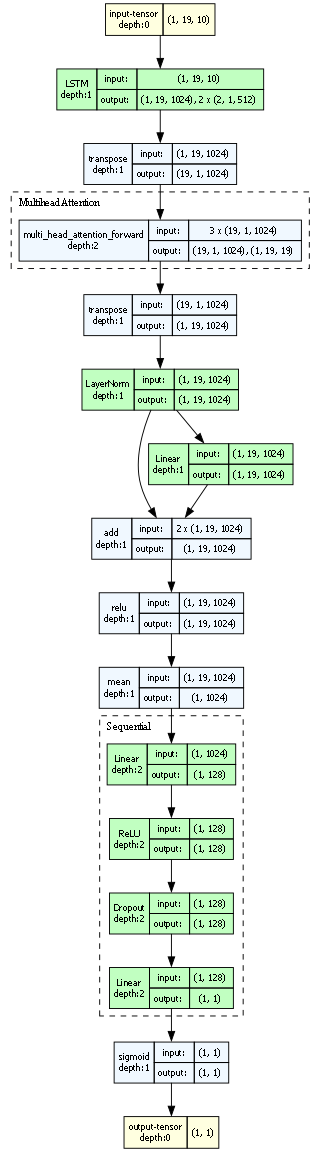
\includegraphics[width=0.4\textwidth]{figures/architecture.png}
  \caption[ResNet-BiLSTM-Attention Architecture]{ResNet-\gls{bilstm}-Attention architecture. Several layers are stacked, including \gls{bilstm}, residual connections, and attention mechanisms. The model processes input sequences, applies self-attention, and outputs a single value for binary classification.}
  \label{fig:architecture}
  \caption*{Source: Own Torchview illustration.}
\end{figure}

The architecture of the ResNet-\gls{bilstm}-Attention model is shown in \autoref{fig:architecture}. The \texttt{torch.nn} module integrates Bidirectional Long Short-Term Memory (\gls{bilstm}) layers with Multi-Head Self-Attention and Residual Connections.

\begin{enumerate}
  \item \textbf{Input/Configuration:} The model is initialized with hyperparameters defining its structure: \texttt{input\_size} (number of input features, $D$), \texttt{hidden\_size} (dimensionality of \gls{lstm} states, $H$), \texttt{num\_layers} (number of stacked \gls{lstm} and Attention blocks, $N$), and \texttt{attention\_heads} (number of parallel attention heads, $A$).

  \item \textbf{\gls{bilstm} Layers:} The core consists of $N$ stacked \gls{bilstm} layers (\texttt{nn.LSTM} with \texttt{bidirectional=True}). Each layer processes the input sequence in both forward and backward directions, capturing dependencies from past and future context. The output dimensionality of each \gls{bilstm} layer is $2H$. Dropout is applied between layers for regularization.

  \item \textbf{Multi-Head Self-Attention:} Following each \gls{bilstm} layer, a \texttt{nn.MultiheadAttention} layer is applied. It performs self-attention on the \gls{bilstm} output sequence, allowing the model to weigh the importance of different time steps relative to each other within the sequence.

  \item \textbf{Layer Normalization \& Residual Connections:} \texttt{nn.LayerNorm} is applied after the attention mechanism within each block to stabilize activations. A residual connection adds the input to this block to the output before a final \texttt{ReLU} activation, facilitating gradient flow in deeper networks.

  \item \textbf{Sequence Pooling:} After the final \gls{lstm}/Attention block, the output sequence (shape: $Batch \times Sequence Length \times 2H$) is aggregated across the sequence dimension using temporal mean pooling (\texttt{torch.mean}), resulting in a single fixed-size vector (shape: $Batch \times 2H$) representing each input sequence.

  \item \textbf{Final Classifier:} A feed-forward network (\texttt{nn.Sequential}) processes the pooled representation. It typically includes one or more linear layers with \texttt{ReLU} activations and Dropout for regularization, culminating in a final linear layer producing a single output logit.

  \item \textbf{Output Activation:} A sigmoid function (\texttt{torch.sigmoid}) is applied to the final logit to produce a probability score between 0 and 1, suitable for binary classification. A threshold $\tau = 0.9$ discriminates the two classes (valid/invalid) during evaluation.

  \item \textbf{Weight Initialization:} Linear layers within the network are initialized using Kaiming Normal initialization (\texttt{nn.init.kaiming\_normal\_}), a standard practice often beneficial for layers followed by \texttt{ReLU} activations.
\end{enumerate}

For training, the model is set to training mode using \texttt{model.train()}. The model weights are updated using the \textit{\gls{adam}} optimizer \texttt{torch.optim.Adam} (\autoref{eq:adam}, \autocite{kingma2014adam}) with an initial learning rate of $0.001$. The loss function employed is binary cross-entropy (\texttt{nn.BCELoss}, \autoref{eq:bce}), which quantifies the difference between the predicted probabilities and the true binary labels. Input data is processed in sequences of length $19$. To prevent overfitting, dropout with a probability of $0.3$ is applied within the \gls{bilstm} layer and also in the final fully connected sequence. The \gls{bilstm} architecture itself consists of $1$ layer (\texttt{num\_layers=$1$}), with a hidden size of $512$ per direction (\texttt{hidden\_size=$512$}). A multi-head attention mechanism with $4$ attention heads (\texttt{attention\_heads=$4$}) is applied after the \gls{bilstm} layer. The final classification head uses an intermediate dense layer with $128$ units before the output neuron. See \autoref{sec:lstm} and following for a description of the theoretical background.

Instead of a fixed learning rate, a learning rate scheduler, specifically \textit{ReduceLROnPlateau} (\texttt{torch.optim.lr\_scheduler.ReduceLROnPlateau}), adjusts the rate during training. This scheduler monitors the training loss and reduces the learning rate by a factor of $0.1$ if the loss does not show improvement for $5$ consecutive epochs (\texttt{patience=$5$}). The model is trained for a default of $10$ epochs (\texttt{num\_epochs=$10$}), iterating over the training dataset in mini-batches of size $32$ (\texttt{batch\_size=$32$}), with shuffling enabled for the training data. In each epoch, the model performs forward and backward passes to compute the loss and gradients, subsequently updating the model parameters via the optimizer. The training loss is tracked per epoch to monitor convergence. The learning rate scheduler in consequence is triggered once after $5$ epochs.\footnote{Using the scheduler was not necessary during the conducted experiments, because the network converged quickly. The learning rate scheduler has rather been introduced for further applications of the framework to facilitate training.}

\section{Model Evaluation}

During evaluation (as seen in \texttt{evaluate\_model}), predicted probabilities are converted to binary labels using a threshold of $\tau = 0.9$. $\tau$ is chosen higher than the default because of the low tolerance for false positives (classifying simulated data as real) in the manufacturing context. Higher thresholds are commonly applied in anomaly detection or when the cost of a false positive is high. This value does not stand in contradiction to the rejection rate ($RR$) derived from the permutation testing (\autoref{sec:permtest}, \autoref{sec:model-logic}). The threshold of $0.9$ is a specific decision boundary for classifying individual instances post-training, impacting metrics like precision and recall at that specific cut-off point. In contrast, the permutation test assesses the overall statistical significance of the difference between the real and simulated data distributions, as captured by the model and features. It uses the \gls{roc} \gls{auc} score, which measures the models ability to distinguish between classes across \textit{all possible thresholds}, not just one. The rejection rate $RR$ then quantifies how consistently this statistically significant difference is found across multiple independent test runs. Therefore, a high $RR$ indicates that the model can reliably detect differences between real and simulated data, regardless of the specific threshold $0.9$ chosen for operational classification based on risk tolerance.
Based on the reference in \autoref{sec:metrics-theory}, the evaluation of the models is performed using various metrics. To achieve this, the model is switched to evaluation mode, \texttt{model.eval()}, to ensure deterministic behaviour. This disables dropout layers so that all neurons are used for the forward pass to achieve predictions. Gradient calculations are disabled through \texttt{torch.no\_grad()}. \texttt{BatchNorm} layers now use their learned estimates of mean and variance parameters to process the data. During evaluation mode, the model processes the test set batch by batch, yielding output probabilities. These are compared against the true labels. The evaluation metrics are implemented in the \texttt{evaluate\_model()} method. The evaluation metrics include a classification report, confusion matrix \autoref{tab:confusionmatrix}, accuracy \autoref{eq:accuracy}, precision \autoref{eq:precision}, recall \autoref{eq:recall}, F1-score \autoref{eq:F1-score} and \gls{roc} \gls{auc} score \autoref{eq:auc}. The metrics are calculated using the \texttt{sklearn.metrics} module. The evaluation metrics are used to compare the performance of the baseline model and the ResNet-\gls{bilstm}-Attention model as well as the standalone performance on the holdout set. The evaluation metrics are also used to diagnose the models and identify potential issues with respect to the bespoken adaptive feature selection procedure. For the assignment of the label 'valid' or 'invalid', a threshold $\tau$ of $0.9$ is used. This value is higher than the usual threshold of $0.5$. This means that if the predicted probability is greater than or equal to $\tau = 0.9$, the process execution is classified as 'valid'. If the predicted probability is less than $0.9$, the process execution is classified as 'invalid'. Setting the boundary so high is a conservative approach. It ensures that only the most confident predictions are classified as 'valid'. This is important for the \gls{vvuq} framework, as it aims to identify potential issues in the process execution. $\tau$ can be adjusted based on the specific requirements of the application and the desired trade-off between precision and recall.\footnote{For anomaly detection, setting $\tau$ higher is a common approach. In different contexts or sectors, lower thresholds may be better. A careful analysis of the \gls{roc} \gls{auc} curve may facilitate finding the best value.} The $0.9$ validity threshold reflects manufacturing \gls{vvuq}'s low tolerance for false positives \autoref{eq:precision}.

\section{Model Evaluation}
\label{sec:model-evaluation}
Based on the reference in \autoref{sec:metrics-theory}, the evaluation of the models is performed using various metrics. To achieve this, the model is switched to evaluation mode using \texttt{model.eval()}, which ensures deterministic behaviour by disabling mechanisms like dropout layers (so all neurons contribute to the forward pass) and configuring \texttt{BatchNorm} layers to use their learned estimates. Gradient calculations are disabled via \texttt{torch.no\_grad()} for efficiency during inference. In this mode, the model processes the test set batch by batch, yielding output probabilities which are then compared against the true labels.

The evaluation metrics, implemented in the \texttt{evaluate\_model()} method using the \texttt{sklearn.metrics} module, include a classification report, confusion matrix (\autoref{tab:confusionmatrix}), accuracy (\autoref{eq:accuracy}), precision (\autoref{eq:precision}), recall (\autoref{eq:recall}), F1-score (\autoref{eq:F1-score}), and the \gls{roc} \gls{auc} score (\autoref{eq:auc}). These metrics serve multiple purposes: Comparing the performance of the bwhitebox model against the ResNet-\gls{bilstm}-Attention model, assessing standalone performance on the holdout set, and diagnosing potential issues related to the adaptive feature selection procedure.

For the practical assignment of the binary labels 'valid' or 'invalid' based on the models output probability, a threshold $\tau$ of $0.9$ is utilized. This value is intentionally set higher than the conventional $0.5$ threshold, reflecting a conservative approach adopted due to the low tolerance for false positives (classifying simulated data as real) within the manufacturing \gls{vvuq} context \autocite[\autoref{eq:precision}]{fahrmeir2016statistik}. If the predicted probability meets or exceeds $\tau = 0.9$, the process execution is classified as 'valid'; otherwise, it is deemed 'invalid'. Setting the boundary high ensures that only highly confident predictions are accepted as 'valid', which is crucial for the framework's goal of identifying potential process deviations. The specific value of $\tau$ can be adjusted depending on application requirements and the desired trade-off between precision and recall.\footnote{For anomaly detection, setting $\tau$ higher is a common approach. In different contexts or sectors, lower thresholds may be better. A careful analysis of the \gls{roc} \gls{auc} curve may facilitate finding the best value.}

It is important to understand that this operational threshold $\tau = 0.9$ serves a different purpose than the rejection rate ($RR$) derived from the permutation testing (\autoref{sec:permtest}, \autoref{sec:model-logic}) and therefore does not stand in contradiction to it. The $\tau = 0.9$ threshold is a specific decision boundary applied \textit{after} training for classifying individual instances, directly impacting metrics like precision and recall calculated at that particular operating point. In contrast, the permutation test assesses the overall statistical significance of the difference between the real and simulated data distributions, as captured by the model and the selected features. This statistical assessment typically uses the \gls{roc} \gls{auc} score, which measures the models ability to distinguish between the classes across \textit{all possible thresholds}, not just the single operational threshold $\tau$. The rejection rate ($RR$) then quantifies how consistently this statistically significant difference is detected across multiple independent test runs. Consequently, a high $RR$ indicates that the model has a fundamental, statistically robust capability to differentiate between real and simulated data, independent of the specific threshold $\tau=0.9$ chosen for practical classification based on risk tolerance.
\chapter{Empirical Validation}
\label{chap:case-study}

The thesis now focuses on the application of the implemented features and methods in a real-world scenario. The goal is to demonstrate the practical applicability of the developed concepts and to validate the theoretical findings presented in the previous chapters.

\section{Physical Entity: Internet of Things Factory}
\label{sec:factory}
The framework has been applied on the Internet of Things-Factory (IOT) in Gütersloh, Germany \autocite{IoTFactory2024}. It is a cyber-physical system (CPS) \autocite{baheti2011cyber} mimicking industry-relevant processes in a smaller scale for research students. It consists of several stations that are partly interconnected via an assembly line or a delivery service conducted by automatic guided vehicles (AGVs). The factory is modular, so processes can be discovered module-wise in isolation. All modules are working on edge but are connected to a cluster that controls them. Theoretically, some stations can perform jobs of others. The main process also evaluated here is circular, meaning that the product is assembled and can be disassembled in a loop. The factory is shown in Figure \ref{fig:iotoverview}.

\begin{figure}[htbp]
  \centering
  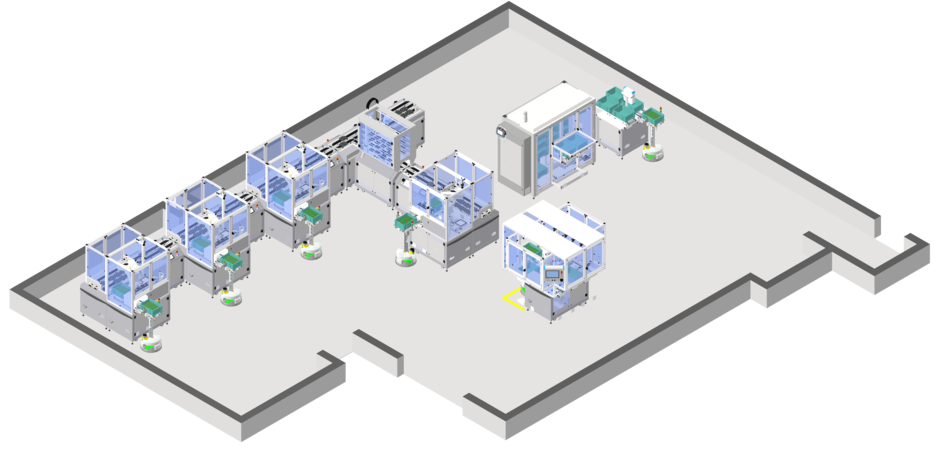
\includegraphics[width=0.7\textwidth]{figures/iot1.png}
  \caption[IoT Factory Overview]{Overview of the IOT factory. It consists of three production stations from left to right, which are followed by a sorting station and a packaging station. The stations are interconnected by an assembly line. Isolated from the assembly part, two AGVs are used to transport parts between the warehouse station (upper right) and another flexible workstation (right).}
  \label{fig:iotoverview}
  \caption*{Source: \autocite{IoTFactory2024}}
\end{figure}

The robot cells are responsible for performing transformation operations like assembling additional parts or testing functions.

\begin{figure}[htbp]
  \centering
  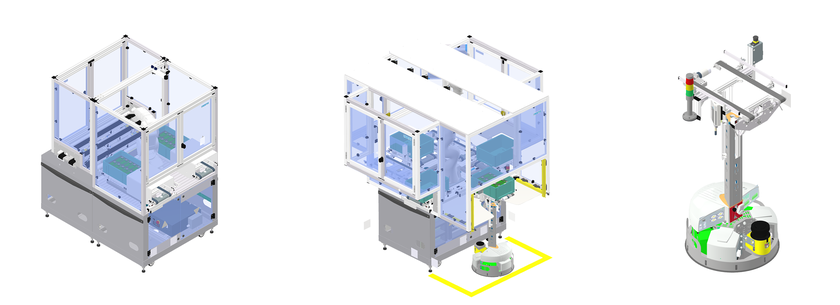
\includegraphics[width=0.8\textwidth]{figures/robots.png}
  \caption[Robot cells]{Two robot cells. The first cell is the main actor in this exemplary production process. Cell two is not part of the observed process here. The third image shows an AGV which transports boxes with assembled and disassembled parts to the stations.}
  \label{fig:robots}
  \caption*{Source: \autocite{IoTFactory2024}}
\end{figure}

The factory produces an exemplary product, consisting of a back part, a breadboard for several parts and a front panel. The parts to put on the breadboard are a display, gyroscope, an analog board and a weather station.

\begin{figure}[htbp]
  \centering
  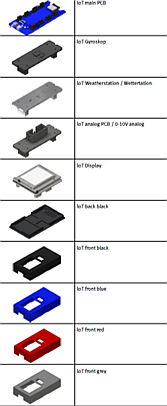
\includegraphics[width=0.2\textwidth]{figures/parts.png}
  \caption[Part variants]{The product consists of a back part, a breadboard and a front panel. The breadboard is used to put on several parts, such as a display, gyroscope, analog board and a weather station.}
  \label{fig:iotproduct}
  \caption*{Source: \autocite{IoTFactory2024}}
\end{figure}

The only colour produced at the moment is black. Not all parts can be put on the breadboard and there are several parts which conflict in size and location on the breadboard. Back and front cover are necessary parts and are assembled every time. The main part \texttt{main\_pcb} is also obligatory. It is placed at the beginning. Following that, the display or gyroscope can be assembled. If the display has been chosen, only the analog board or the weather station can be assembled. The weather station takes too much space on the breadboard for the gyroscope to be placed. If the analog board has been placed, the gyroscope is of course possible. The product is finished by placing the front cover and delivering the product to the sink.During the production, the factory gathers data via sensors. The data is saved in a database and can be used for further analysis. The database is relational and supports SQL queries.

Finally, the sequential order of the production process is as follows:

\begin{figure}[H]
  \centering
  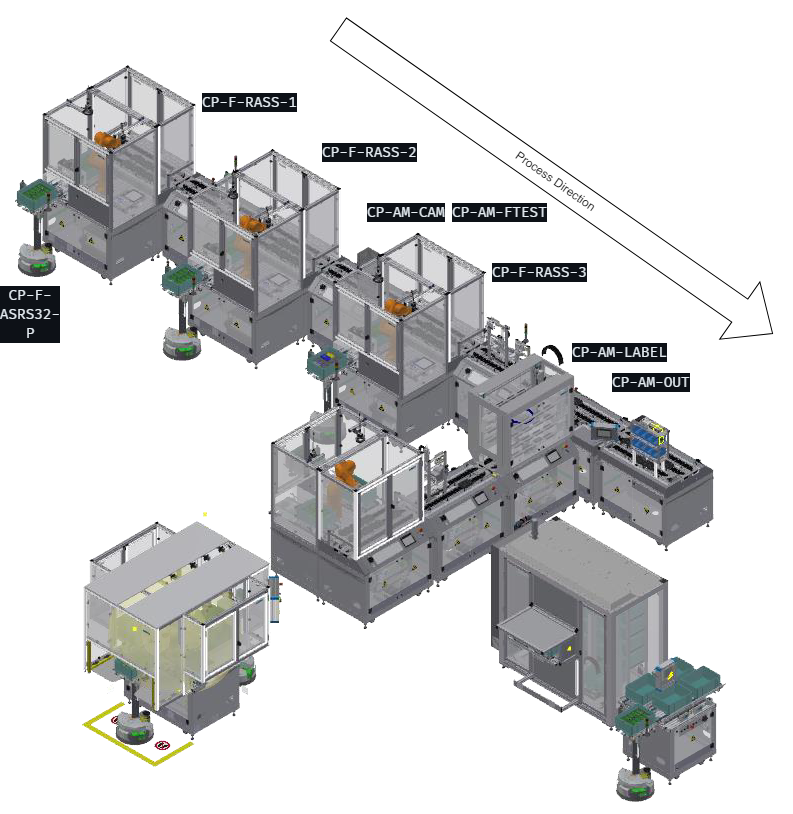
\includegraphics[width=0.7\textwidth]{figures/processdirection.png}
  \caption[Production process]{The blueprint with transitions between resources.}
  \label{fig:transitions}
  \caption*{Source: \autocite{IoTFactory2024}}
\end{figure}

\subsection*{Factory Dataset}

The dataset has been gathered from the database of the IoT Factory. In the code it is referred to as \texttt{real\_data}.

The dataset contains 18057 rows and 4696 orders from a time span of 22.04.2020 to 14.05.2024. There are no duplicate rows. Each row describes a unique operation step in an order. Roughly 40 percent of the rows contain missing values, which have been filled with zeros. The data has been mined from a MariaDB SQL database of the IoT Factory. Several tables have been aggregated to form the dataset. Without additional tables, no information about workplans, resources and operation numbers would be available. The dataset is filtered for promising trajectories of meaningful and intact process executions. The filter considers data between the 20.04.2020 and 22.04.2022, 02.05.2022 and 19.07.2022, 02.11.2022, 11.11.2022, 23.01.2022 and March 2023, each data inclusively.

The dataset contains the following columns:

\begin{itemize}
  \item \textbf{WPNo}: The workplan number of the specific workplan.
  \item \textbf{StepNo}: The step number of the specific workplan. The workplan is divided in sequential steps enumerated by this number.
  \item \textbf{ONo}: The order number of the specific order. Each order has a unique number.
  \item \textbf{OPos}: The order position of the specific order. The order position is the position of the order in the workplan.
  \item \textbf{Description}: The description of the specific step in spoken language.
  \item \textbf{OpNo}: The operation number of the specific operation. Each operation has a unique number.
  \item \textbf{NextStepNo}: The next step number of the specific step. This is the step that follows the current step.
  \item \textbf{FirstStep}: The first step of the specific workplan.
  \item \textbf{ErrorStepNo}: The error step number of the specific step. This is the step that is executed in case of an error.
  \item \textbf{Start}: The start time of the specific step.
  \item \textbf{End}: The end time of the specific step.
  \item \textbf{OPNoType}: The operation number type of the specific operation.
  \item \textbf{ResourceID}: The resource ID of the specific resource.
  \item \textbf{ErrorStep}: Is this step an error step (yes/no)?
  \item \textbf{ErrorRetVal}: The error return value of the specific step.
  \item \textbf{Active}: Is this step active (yes/no)?
  \item \textbf{op\_desc}: The operation description of the specific operation, which is more specific than the description.
  \item \textbf{ResourceName}: The name of the specific resource.
  \item \textbf{resource\_desc}: The description of the specific resource.
  \item \textbf{workplan\_desc}: The description of the specific workplan.
  \item \textbf{workplantype\_desc}: The description of the specific workplan type.
  \item \textbf{case\_id}: The case ID of the specific case.
  \item \textbf{Description\_Encoded}: The description of the specific step ordinally encoded.
\end{itemize}

The operations performed can be seen in the following:

\begin{enumerate}
  \item \textbf{Release a part on stopper 1}: The AGV delivered the box with the parts to be manufactured to the first station. The box is travelling over the assembly line to the first station where the first part is released.
  \item \textbf{Place cover to assembly place}: The first part is placed on the assembly place. The cover is placed on top of the part as the first piece of the product.
  \item \textbf{Assemble part from box on RASS1 - MAIN PCB}: The main PCB is assembled on the cover. This is the first configured part of the product. The main PCB is the breadboard of the product.
  \item \textbf{Switch on PCB}: The main PCB is switched on. This is necessary to activate it.
  \item \textbf{Assemble part from box on RASS1 - DISPLAY}: The display is assembled on the main PCB. This is the second configured part of the product. The display is one optional part of the product. This factors out one product variant.
  \item \textbf{Move part to pallet on belt}: The product is moved to the pallet on the belt for further processing.
  \item \textbf{Measure a part (analog)}: The product is measured. This is necessary to ensure the quality of the product for later steps.
  \item \textbf{Assemble part from box on RASS2 - ANALOG}: The analog part is assembled on the product. This is the third configured part of the product. The analog part is also one optional part of the product.
  \item \textbf{Assemble part from box on RASS2 - GYROSCOPE}: The gyroscope is assembled on the product. This is the fourth configured part of the product. The gyroscope is also one optional part of the product.
  \item \textbf{Move part to pallet on belt}: The product is moved to the pallet on the belt for further processing.
  \item \textbf{Check analog}: The analog part is checked. This is necessary to ensure the quality of the product for later steps.
  \item \textbf{Check gyroscope}: The gyroscope is checked. This is necessary to ensure the quality of the product for later steps
  \item \textbf{Assemble part from box on RASS3 - FRONT COVER}: The front cover is assembled on the product. This is the last configured part of the product. The front cover is the last part of the product.
  \item \textbf{Move part to pallet on belt}: The product is moved to the pallet on the belt for further processing.
  \item \textbf{Test connection to IoT main PCB}: The connection to the IoT main PCB is tested. This is necessary to ensure the quality of the product for later steps.
  \item \textbf{Test the function of the touch display}: The touch display is tested. This is necessary to ensure the quality of the product for later steps.
  \item \textbf{Test the analog input/output shield}: Analog PCB is tested.
  \item \textbf{Test the historical gyroscope data}: The gyroscope is tested.
  \item \textbf{Print Label}: The label is printed. The label contains information about the product configuration, the time manufactured and the serial number.
  \item \textbf{Deliver Part}: The final product is delivered to the sink.
\end{enumerate}

Per step, several resources are involved. The following table shows the utilized resources per step:

\begin{table}[H]
  \centering
  \footnotesize
  \caption[Production steps and resources]{Steps and Resources Used}
  \label{tab:description-resources}
  \begin{tabular}{@{}p{0.4\textwidth}p{0.4\textwidth}@{}}
    \toprule
    \textbf{Process Step Name}                    & \textbf{Resource Name}                \\
    \midrule
    Release a part on stopper 1                   & CP-F-ASRS32-P                         \\
    Place cover to assembly place                 & CP-F-RASS-1, CP-F-RASS-2, CP-F-RASS-3 \\
    Assemble part from box on RASS1 - MAIN PCB    & CP-F-RASS-1                           \\
    Switch on PCB                                 & CP-F-RASS-1                           \\
    Assemble part from box on RASS1 - DISPLAY     & CP-F-RASS-1                           \\
    Move part to pallet on belt                   & CP-F-RASS-1, CP-F-RASS-2, CP-F-RASS-3 \\
    Measure a part (analog)                       & CP-AM-MEASURE                         \\
    Assemble part from box on RASS2 - ANALOG      & CP-F-RASS-2                           \\
    Assemble part from box on RASS2 - GYROSCOPE   & CP-F-RASS-2                           \\
    Move part to pallet on belt                   & CP-F-RASS-1, CP-F-RASS-2, CP-F-RASS-3 \\
    Check analog                                  & CP-AM-CAM                             \\
    Check gyroscope                               &                                       \\
    Assemble part from box on RASS3 - FRONT COVER & CP-F-RASS-3                           \\
    Move part to pallet on belt                   & CP-F-RASS-1, CP-F-RASS-2, CP-F-RASS-3 \\
    Test connection to IoT main PCB               & CP-AM-FTEST                           \\
    Test the function of the touch display        & CP-AM-FTEST                           \\
    Test the analog input/output shield           & CP-AM-FTEST                           \\
    Test the historical gyroscope data            & CP-AM-FTEST                           \\
    Print Label                                   & CP-AM-LABEL                           \\
    Deliver Part                                  & CP-AM-OUT                             \\
    \bottomrule
  \end{tabular}
  \caption*{Source: \Textcite{IoTFactory2024}}
\end{table}


This process has been identified as the ground-truth process. The process is circular, meaning that the product is assembled and can be disassembled in a loop. The process is also modular, so that the product can be assembled in different configurations. The process is also flexible, the product can be assembled in different ways.

\section{Digital Entity: Open Factory Twin}
\label{sec:automated-digital-twin}

The Simulation-Based Digital Twin (SBDT) for the IoT Factory use case was developed using the Open Factory Twin (OFacT) framework \autocite{ofact-intern}. OFacT is an open-source digital twin framework specifically designed for modelling, simulating, and controlling production and logistics environments. Its goal is to support system design, planning, and operational control during the entire lifecycle of such systems.

A principle of OFacT is the separation between the static description of the system and its dynamic behaviour. This is achieved by distinguishing between:

\begin{itemize}
  \item \textbf{State Model:} This component represents the static structure of the factory, its components (resources, parts, layout), their properties, relationships, and the potential processes or behaviours they can exhibit.
  \item \textbf{Agent Control:} This component implements the dynamic logic that controls the systems operation during simulation, making decisions about resource allocation, process execution sequences, and handling events based on the state model.
\end{itemize}

The construction of the State Model within OFacT uses structured input methods, such as Excel files, where different sheets correspond to specific classes within the OFacT metamodel, inspired by \textcite{schwede2024learning}. To model the IoT Factory scenario (\autoref{sec:factory}), the relevant components of the OFacT State Model were defined, including:

\begin{itemize}
  \item \textbf{Plant}: The overall entity of production. The plant name used here was \texttt{iot\_factory}.
  \item \textbf{EntityType}: All entities have to be defined here. This ranges from the parts, resources and AGVs to the factory itself.
  \item \textbf{StationaryResource}: Stationary resources are static and can not move. In this case, these are the RASS stations, measurement-, cam-, function test- and labelling station. The AGVs are not stationary resources, because they can move.
  \item \textbf{Storage}: Storage units contain parts. They are used to traverse the parts through the factory. In this context, the warehouse and box storage, have been modelled.
  \item \textbf{Warehouse}: This is a static storage unit where the parts are stored in boxes until they are processed.
  \item \textbf{WorkStation}: Workstations are resources which perform processes on parts. In our use case, these are the RASS stations.
  \item \textbf{ConveyorBelt}: There is one belt where the storage units traverse through the factory.
  \item \textbf{NonStationaryResource}: There are no non-stationary resources.
  \item \textbf{PassiveMovingResource}: One artificial passive moving resource has been mod
  \item \textbf{Process}: Contains processes and value added processes (VAP). VAP are adding features to parts and modify it. For each activity in the data a VAP has been created.
  \item \textbf{ProcessController}: This controller summarizes all processes to come and connects them.
  \item \textbf{ResourceModel}: Resource groups are formulated for activities like montage, identifying to attach the relevant parts to these resources. This way, main resources and parts are getting matched.
  \item \textbf{ProcessTimeModel}: Each part receives a time simple time distribution to account for its production time.
  \item \textbf{QualityModel}: Each part receives a bernoulli distribution to account for its quality. In the dataset, no quality information existed.
  \item \textbf{TransitionModel}: This model connects possible origins to possible destinations, to that the traversal of the parts can be modelled correctly. The packaging has been modelled as transition model.
  \item \textbf{TransformationModel}: This model contains an artificial transformation model.
  \item \textbf{Time}: Process execution plans get a starting time here.
  \item \textbf{Part}: Parts are connected to their EntityType here. There is also information attached where the part is stored or situated in.
  \item \textbf{Sales}: Lists the features and feature cluster. This matches the building rules. Parts have to be defined as features here.
  \item \textbf{CustomerGeneration}: Customer generation logic.
  \item \textbf{Customer}: List of customers.
  \item \textbf{Orders}: The orders with their requested features.
  \item \textbf{Process}: Contains processes and value added processes (VAP). VAP are adding features to parts and modify it. For each activity in the data a VAP has been created.
  \item \textbf{TransitionModel}: This model connects possible origins to possible destinations, to that the traversal of the parts can be modelled correctly. The packaging has been modelled as transition model.
  \item \textbf{TransformationModel}: This model contains an artificial transformation model.
\end{itemize}

By defining these elements according to the IoT Factory characteristics, a detailed static model was created within the OFacT framework. For simulation purposes, the state model then gets played out \autoref{fig:playinoutreplay} with orders. The orders contain this model then served as the basis for running simulations to generate process execution data, forming the SBDT dataset used in this thesis for comparison against real-world data.

\subsection*{SBDT Dataset}

The dataset gathered from the SBDT is referred to as \texttt{sim\_data}. The OpenFactoryTwin provides a method to deserialize the simulated orders and save them in a CSV file. The dataset then gets converted to the OCEL structure. For this endeavour, a separate connector logic has to be implemented in every use case.\footnote{See \texttt{src/connector/ofact} for the connector here.}

The connector's output follows a standardized structure defined by the \texttt{OutputStructure} class, which ensures consistency across different data sources. The connector first deserializes the dynamic state model from a pickle file, accessing the full simulation state. Only actual process executions (not planned ones) are kept for further processing, identified by the `ACTUAL' flag in their event type. The connector creates mapping dictionaries for various categorical attributes following the OCED standard. The categories can be defined by the modeller beforehand, which is the case here. The IDs are based on enumeration and default to -1 if the category has not been found in the list:

\begin{itemize}
  \item \textbf{Part ID Mapping:} Uses domain expertise to identify part types from process names, normalizing text (lowercase, no whitespace) to match against a predefined list of possible parts. This list contains possible parts from \autoref{fig:iotproduct}.
  \item \textbf{Process Type Categorization:} Assigns process steps to expert-defined categories such as `machine,' `feature,' `endproduct,' `test,' and `transport' based on keywords in process names. These types have been assigned by the modeller and are of free choice.
  \item \textbf{Process ID Mapping:} Creates unique integer identifiers for each distinct process description based on enumeration.
  \item \textbf{Resource ID Mapping:} Generates unique identifiers for each resource involved in the process executions based on enumeration.
  \item \textbf{Temporal Data Extraction:} The connector extracts start and end times for each process execution.
\end{itemize}

Process executions are associated with their respective order IDs, establishing the connection between individual process steps and the orders they belong to. All extracted information is then consolidated into a standardized DataFrame structure with properly typed columns as defined in the \texttt{OutputStructure} class. The connector also includes a validation step to ensure that the generated DataFrame adheres to the expected structure and data types, raising an error if any discrepancies are found.

A key aspect of the connector's functionality is the non-mandatory integration of domain knowledge into the data transformation process. Instead of relying only on the raw data structure, the connector employs expert-defined categorizations and normalization procedures to ensure semantic consistency in the transformed data.

For example, the part identification logic uses a predefined list of potential parts (such as `GYROSCOPE,' ``MAIN PCB,' ``FRONT COVER,' etc.) and searches for these terms within process descriptions. Similarly, the process type categorization uses domain-specific groupings like `machine,' `feature,' and `test' based on keywords found in process names. The \texttt{sim\_data} rows will receive the label $0$ for \texttt{is\_valid}, because the black-box model should learn to distinguish between real and simulated data to perform VVUQ. The entries of the \texttt{real\_data} receive $1$ for \texttt{is\_valid}.


\section{Data Pipeline}
\label{sec:data-pipeline}

Several preprocessing steps had to be performed to account for the fact that the SBDT simulated only one variant of the product: 'analog', 'cover', 'display', 'gyroscope', 'pcb' and the involved machines. This yielded the necessity to make both datasets congruent to each other. The following steps were performed:

\begin{itemize}
  \item The \texttt{sim\_data} dataset was aligned for the same time period as the \texttt{real\_data} dataset. The SBDT chose the time of order as the production time. In the modelling phase, when adaptive feature selection had been performed to identify if the SBDT was able to learn the Time Model, only \textit{relative} time features like duration were chosen which were developed in \autoref{sec:feature-engineering}.
  \item The \texttt{real\_data} dataset was filtered for the same process steps as the \texttt{sim\_data} dataset. This means that only the process steps which are present in the \texttt{sim\_data} dataset were kept, producing only one product variant. This has also been applied on the part\_id, the process\_type and resource\_id columns. The IDs based on enumeration had to be mapped to the original IDs in \texttt{real\_data} to ensure that the correct IDs are used in the simulation. The mapping was done through the JSON files generated by the connector.
  \item Both datasets have been cleaned and entries containing invalid IDs were removed. This means that all entries which are not present in the mapping dictionaries were removed. The mapping dictionaries are generated by the connector and contain only valid IDs per definition.
  \item Only a subset of all performed processes was included (in detail, all \texttt{process\_id} $\le 26$). These processes all have the \texttt{process\_type} 'machine', 'feature' or 'endproduct'. The processes with the \texttt{process\_type} 'test' and 'transport' were removed. This was done to ensure that only the relevant processes are included in the dataset.
\end{itemize}

This cleaning step was not corrupting the data to facilitate easier learning of the models, it removed epistemic uncertainty. For example, some rows contained invalid names.
The \texttt{real\_data} dataset was then concatenated with the \texttt{sim\_data} dataset. The concatenation was done by appending the \texttt{sim\_data} dataset to the \texttt{real\_data} dataset. The resulting dataset contains all process steps from both datasets. The resulting dataset is referred to as \texttt{final\_data}. The unification before concatenation was necessary to ensure that no logical flaws are present in the data.

The \texttt{final\_data} dataset after preprocessing as described contains 1978 rows and 56 orders with 24 features. The following section elaborates how these features were generated.

\subsection*{Feature Engineering}
\label{sec:feature-engineering}

Several features have been engineered to assist both the whitebox and blackbox model on the validation task. The features were furher introduced to empower adaptive feature selection (AFS) regarding the model components of the SBDT \autocite{schwede2024learning}. This way, if the features sufficiently explain the data, the conclusion can be made that the SBDT was able to learn the respective model component.

The following features were generated with domain knowledge:

\begin{itemize}
  \item \textbf{KPIs}: Throughput, setup time, lead time and cycle time have been added to assist the VVUQ, see \autoref{sec:relevant-kpis}. They allow PPC VVUQ to be performed. They further can be integrated to check if the Time Model has been learned.
  \item \textbf{duration}: The duration of the process step. This feature is important to understand how long the process step took. It is calculated as the difference between the start and end time of the process step.
  \item \textbf{sequence\_number}: The sequence number of the process step. This feature is important to understand the order of the process steps. It is calculated by grouping the data by the process execution ID and then enumerating the process steps within each group based on the end time. This way, the sequence number enumerates each process step per order. It helps the \texttt{DecisionTreeClassifier} to learn the order of the process steps.
  \item \textbf{is\_not\_weekday}: A binary feature indicating whether the process step occurred on a weekend (1) or a weekday (0). No activities have been performed on weekends in the factory, so weekend activity is an anomaly.
  \item \textbf{is\_break}: A binary feature indicating whether the process step occurred during a break (1) or not (0). No activities have been performed during breaks in the factory, so break activity is an anomaly as well.
  \item \textbf{hour\_of\_day}: The hour of the day when the process step occurred. This feature is important to understand the time of day when the process step took place. It is calculated as the hour of the start time of the process step.
  \item \textbf{day\_of\_week}: The day of the week when the process step occurred. It is also calculated as the day of the week of the start time of the process step.
  \item \textbf{day\_of\_week\_sin and day\_of\_week\_cos}: A periodic time feature representing the sine and cosine of the day of the week, which helps capture weekly patterns in the data.
  \item \textbf{hour\_of\_day\_cos and hour\_of\_day\_sin}: A periodic time feature representing the cosine and sine of the hour of the day, which helps capture daily patterns in the data.
\end{itemize}

Days and hours are cyclical features that require special handling. Representing them as raw integers fails to capture their continuity (e.g., hour 23 is close to hour 0). To address this, the feature $x$ with period $P$ using sine and cosine functions has been transformed, effectively mapping it onto a unit circle:
\begin{equation}
  x_{\sin} = \sin\left(\frac{2 \pi x}{P}\right) \quad ; \quad
  x_{\cos} = \cos\left(\frac{2 \pi x}{P}\right)
  \label{eq:sincos_transform}
\end{equation}
This provides a continuous, two-dimensional representation $(x_{\cos}, x_{\sin})$ that preserves the cyclical nearness of values.

In this work, this transformation is applied to:

\begin{itemize}
  \item \textbf{Hour of Day (`hour\_of\_day`):} $P=24$. Features: $\text{hour\_of\_day}_{\sin}$, $\text{hour\_of\_day}_{\cos}$.
  \item \textbf{Day of Week (`day\_of\_week`):} $P=7$. Features: $\text{day\_of\_week}_{\sin}$, $\text{day\_of\_week}_{\cos}$.
\end{itemize}

Figure \ref{fig:time-encoding} illustrates this concept for the hour of the day. This encoding helps machine learning models better understand and utilize the cyclical nature of time.

\section{Validation Methodology and Setup}
With the integration of these features, AFS can be performed. For the statistical soundness of the analysis, a permutation test will be performed to assess the significance of the results. The following sections outline the testing procedure and the specific components of the SBDT that will be evaluated.

\subsection*{Permutation Testing for Statistical Significance}
\label{sec:model-logic}

As laid out in the methodology chapter \autoref{sec:permtest}, a permutation test will be conducted.

\noindent The null hypothesis ($H_0$) claims that the SBDT accurately represents the real system with respect to the features $\mathcal{F}_c$, meaning the data distributions are indistinguishable:
\begin{equation}
  H_0: \mathcal{D}_{real}(\mathbf{X} | \mathcal{F}_c) = \mathcal{D}_{sim}(\mathbf{X} | \mathcal{F}_c)
  \label{eq:h0}
\end{equation}

\noindent The alternative hypothesis ($H_1$) claims that the SBDT does \textit{not} accurately represent the real system, and the distributions are statistically distinguishable using the features $\mathcal{F}_c$:
\begin{equation}
  H_1: \mathcal{D}_{real}(\mathbf{X} | \mathcal{F}_c) \neq \mathcal{D}_{sim}(\mathbf{X} | \mathcal{F}_c)
  \label{eq:h1}
\end{equation}

\noindent Under this framework, if a classifier trained on the feature set $\mathcal{F}_c$ achieves performance significantly better than chance at distinguishing between real ($y=1$) and simulated ($y=0$) data, it provides evidence to reject $H_0$ in favour of $H_1$. This would imply that the SBDT component $c$ has \textit{not} been learned accurately, as detectable discrepancies exist. Conversely, if the classifier performs poorly (close to random chance), it fails to reject $H_0$, suggesting that, based on the features $\mathcal{F}_c$, the simulated data is consistent with the real data for that component.

\subsection*{Testing the SBDT Components}
To rigorously evaluate the SBDTs fidelity concerning different process aspects, the thesis implements the hypothesis testing framework outlined previously (testing $H_0$: \autoref{eq:h0} against $H_1$: \autoref{eq:h1}). This involved using machine learning classifiers to determine if statistically significant differences exist between the real process data ($\mathcal{D}_{real}$, labelled $y=1$) and the simulated data ($\mathcal{D}_{sim}$, labelled $y=0$) based on specific feature subsets ($\mathcal{F}_c$) corresponding to key SBDT model components.

The analysis was performed separately for distinct feature subsets $\mathcal{F}_c$, each clustered to reflect the behavior exhibited by specific SBDT components. Based on the feature engineering described in \autoref{sec:feature-engineering}, several targeted feature sets were defined. The \texttt{time\_model} subset encompasses temporal patterns and cyclical time representations, including \texttt{duration}, \texttt{sequence\_number}, cyclical encodings (\texttt{hour\_of\_day\_cos}, \texttt{hour\_of\_day\_day\_sin}, \texttt{day\_of\_week\_cos}, \texttt{day\_of\_week\_sin}), and temporal status indicators (\texttt{is\_break}, \texttt{is\_not\_weekday}). For operational resource allocation, the \texttt{resource\_model} subset includes categorical identifiers (\texttt{resource\_id}, \texttt{part\_id}, \texttt{process\_id}). To capture product transformations, the \texttt{transformation\_model} subset contains \texttt{part\_id}, \texttt{process\_id}, and \texttt{sequence\_number}. Movement patterns are represented in the \texttt{transition\_model} subset through \texttt{part\_id}, \texttt{resource\_id}, \texttt{sequence\_number}, and \texttt{duration}. Process execution characteristics are encapsulated in the \texttt{process\_model} subset via \texttt{process\_id}, \texttt{duration}, and \texttt{sequence\_number}. Additionally, the \texttt{kpi\_based} subset includes performance indicators (\texttt{throughput}, \texttt{cycle\_time\_sec}, \texttt{lead\_time\_sec}, \texttt{setup\_time\_sec}). Finally, an \texttt{all\_features} set combined all available engineered features to provide a comprehensive perspective.

\subsection*{Permutation Testing Procedure}

The practical implementation of the test described in \autoref{eq:pvalue_perm} followed these steps for each feature subset $\mathcal{F}_c$:

\begin{algorithm}[H]
  \caption[Permutation Testing]{Multi-Run Permutation Testing}
  \label{alg:permutation_testing_symbolic}
  \begin{algorithmic}[1]
    \footnotesize % Font size
    % -----------

    \Require % Input:
    \Statex \hspace{\algorithmicindent} Concatenated Dataset $\mathcal{D}_{final}$ (Features $\mathbf{X}$, Labels $y \in \{0,1\}$),
    \Statex \hspace{\algorithmicindent} Feature Subsets for model components $\{\mathcal{F}_c\}_{c=1}^C$,
    \Statex \hspace{\algorithmicindent} Runs $n_{runs}$, Permutations $N$, Significance level $\alpha$, Model Type $M_{type}$ \Comment{DTree, BiLSTM}
    \Ensure % Output:
    \Statex \hspace{\algorithmicindent} Results $R : \{c \mapsto (\bar{S}_{obs}, \sigma_{S_{obs}}, \bar{p}, RR)\}$ \Comment{Map component to aggregated stats}
    \medskip

    \State $R := \emptyset$ \Comment{Initialize results map}
    \medskip

    \ForAll{feature subset $\mathcal{F}_c$ for component $c$}
    \State $S_{obs\_list} := [\,]$; $p_{list} := [\,]$ \Comment{Initialize arrays for run results}
    \medskip
    \For{$run = 1$ to $n_{runs}$}
    \State $seed \leftarrow \text{RandomSeed}()$
    \State $(\mathcal{D}_{train}, \mathcal{D}_{test}) \leftarrow \text{Split}(\mathcal{D}_{final}, \mathcal{F}_c, seed)$ \Comment{Split stratified on $y$}
    \State $M \leftarrow \text{Train}(M_{type}, \mathcal{D}_{train})$ \Comment{Train on $(\mathbf{X}_{train}, \mathbf{y}_{train})$ using features $\mathcal{F}_c$}
    \medskip

    \State $\hat{\mathbf{p}}_{test} \leftarrow M(\mathbf{X}_{test})$ \Comment{Predict $P(y=1|\mathbf{X}_{test})$ using trained model $M$}
    \State $S_{obs} \leftarrow \text{ROC\_AUC}(\mathbf{y}_{test}, \hat{\mathbf{p}}_{test})$ \Comment{Observed score}
    \medskip

    \State $S_{perm\_list} := [\,]$
    \For{$i = 1$ to $N$}
    \State $\mathbf{y}_{test, perm}^{(i)} \leftarrow \text{Permute}(\mathbf{y}_{test})$ \Comment{Randomly shuffle test labels}
    \State $S_{perm, i} \leftarrow \text{ROC\_AUC}(\mathbf{y}_{test, perm}^{(i)}, \hat{\mathbf{p}}_{test})$ \Comment{Score vs fixed $\hat{\mathbf{p}}_{test}$}
    \State Append $S_{perm, i}$ to $S_{perm\_list}$
    \EndFor
    \medskip

    \State $count_{ge} \leftarrow \sum_{i=1}^{N} \mathbb{I}(S_{perm\_list}[i] \ge S_{obs})$
    \State $p_{run} \leftarrow count_{ge} / N$ \Comment{p-value for this run}
    \medskip

    \State Append $S_{obs}$ to $S_{obs\_list}$; Append $p_{run}$ to $p_{list}$ \Comment{Store run results}
    \EndFor \Comment{End runs}
    \medskip

    \State $\bar{S}_{obs} \leftarrow \text{Mean}(S_{obs\_list} | \text{not NaN})$ \Comment{Calculate mean of valid observed scores}
    \State $\sigma_{S_{obs}} \leftarrow \text{StdDev}(S_{obs\_list} | \text{not NaN})$ \Comment{Calculate $\sigma$ of valid observed scores}
    \State $\bar{p} \leftarrow \text{Mean}(p_{list} | \text{not NaN})$ \Comment{Calculate mean of valid p-values}
    \State $RR \leftarrow \text{Mean}(\mathbb{I}(p < \alpha) \mid p \in p_{list}, p \neq \text{NaN})$ \Comment{Rejection Rate on valid p-values}
    \State $R[c] \leftarrow (\bar{S}_{obs}, \sigma_{S_{obs}}, \bar{p}, RR)$ \Comment{Store aggregated results for component $c$}
    \medskip
    \EndFor \Comment{End feature subsets}

    \State \Return $R$

  \end{algorithmic}
\end{algorithm}

\begin{enumerate}
  \item \textbf{Data Splitting:} The combined dataset (\texttt{final\_data}) was split into stratified training ($\mathcal{D}_{train}$) and testing ($\mathcal{D}_{test}$) sets, ensuring proportional representation of real ($y=1$) and simulated ($y=0$) data in both sets. A random seed was used for reproducibility within a single run.
  \item \textbf{Model Training:} The chosen classifier (DTree or BiLSTM) was trained on $\mathcal{D}_{train}$ using only the features in $\mathcal{F}_c$.
  \item \textbf{Observed Statistic Calculation:} The trained model was evaluated on the original test set $\mathcal{D}_{test}$. The performance metric, specifically the ROC AUC score \autoref{eq:auc}, was calculated and recorded as the observed statistic, $S_{obs}$.
  \item \textbf{Null Distribution Generation (Permutation):} To generate the null distribution, $N$ permutations were performed. Critically, an efficient approach was used, particularly for the computationally intensive BiLSTM model:
        \begin{itemize}
          \item The trained model generated predictions (binary $\hat{\mathbf{y}}_{test}$) and class probabilities (specifically for the positive class, $\hat{\mathbf{p}}_{test}$) on the original test set $\mathcal{D}_{test}$ \textit{once}.
          \item For each permutation $i=1...N$: The *true labels* $\mathbf{y}_{test}$ of the test set were randomly shuffled, creating $\mathbf{y}_{test, perm}^{(i)}$.
          \item The permuted statistic $S_{perm, i}$ was calculated by comparing the shuffled labels $\mathbf{y}_{test, perm}^{(i)}$ against the fixed probabilities $\hat{\mathbf{p}}_{test}$ (i.e., calculating ROC AUC between $\mathbf{y}_{test, perm}^{(i)}$ and $\hat{\mathbf{p}}_{test}$). This avoids retraining the model for each permutation. (A similar principle was applied for the Decision Tree, comparing permuted labels against fixed predictions/probabilities).
        \end{itemize}
  \item \textbf{P-value Calculation:} The p-value was computed as the proportion of permutation statistics greater than or equal to the observed statistic, following \autoref{eq:pvalue_perm}.
        \begin{equation}
          p = \frac{\sum_{i=1}^{N} \mathbb{I}(S_{perm, i} \ge S_{obs})}{N}
          \nonumber
        \end{equation}
\end{enumerate}

\section{Results and Interpretation}
The feature subsets are equal to the model components, as noted. The following UpSet plot summarizes the feature subsets used for the SBDT components.

\begin{figure}[htbp]
  \centering
  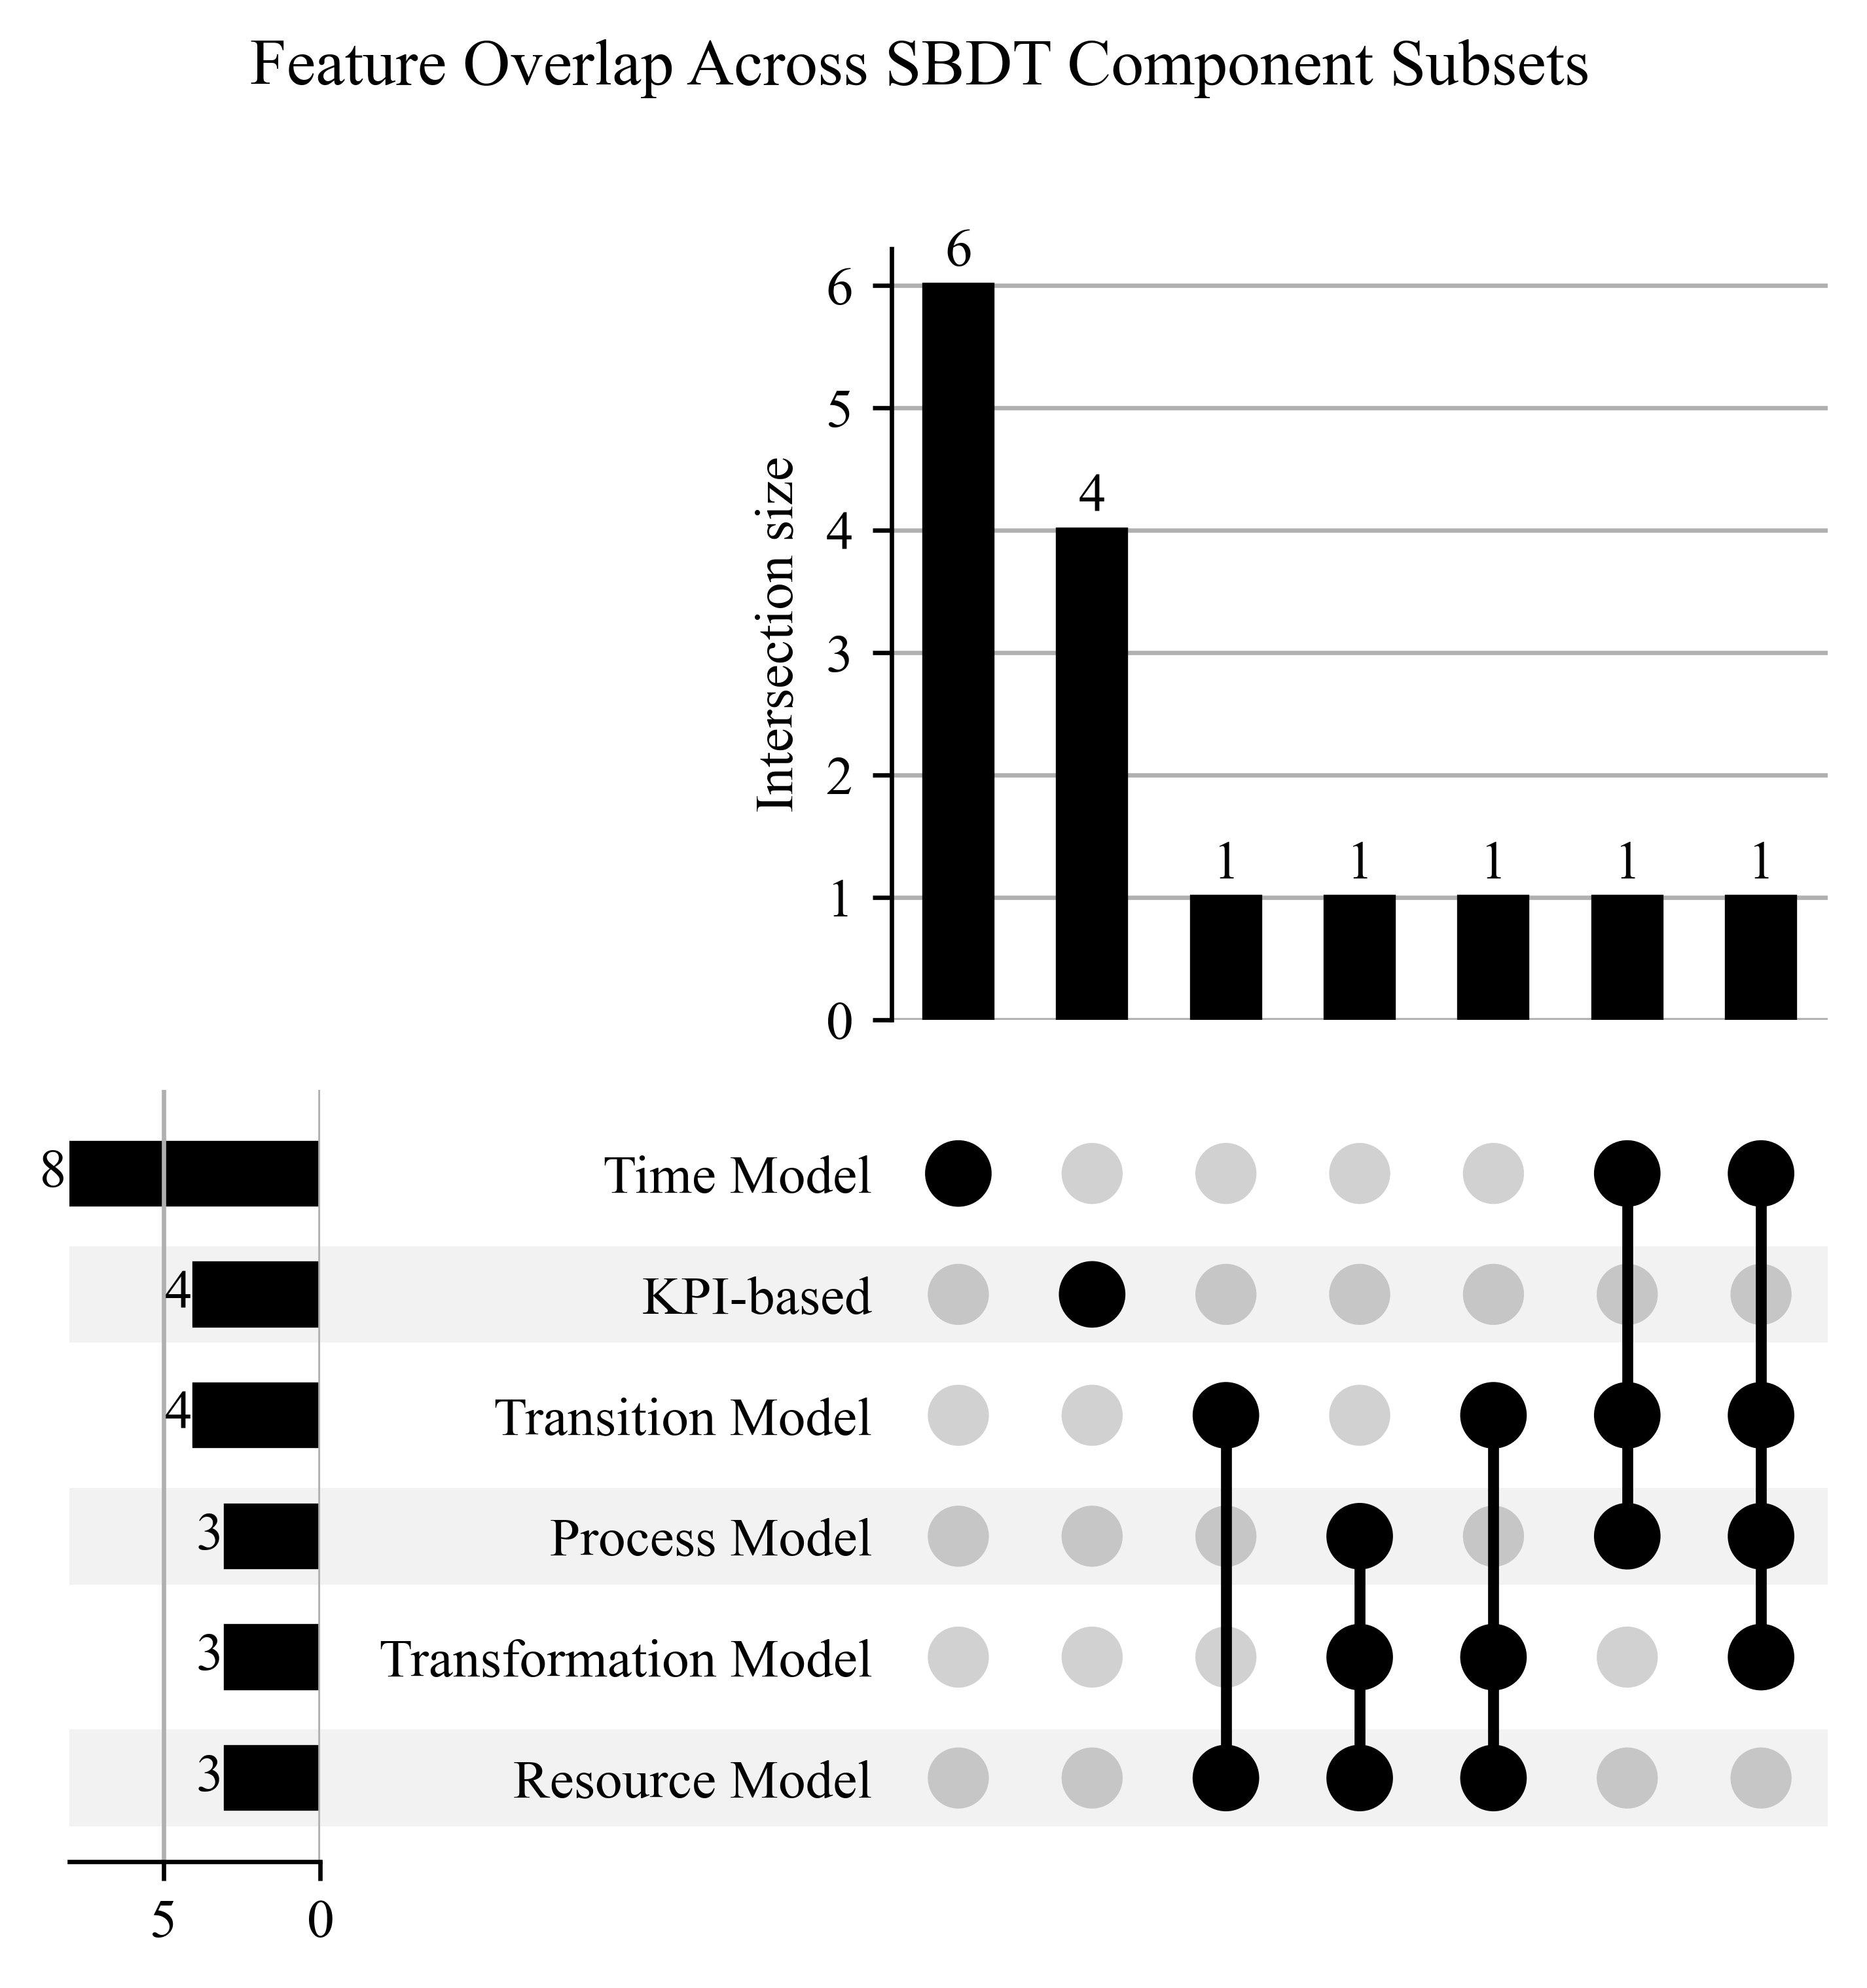
\includegraphics[width=0.7\textwidth]{figures/upset.png}
  \caption[UpSet plot]{UpSet plot visualizing feature overlap across categories. Left bars show total features per category; top bars show counts for specific intersections defined by the dot matrix below.}
  \caption*{Source: Own illustration.}
  \label{fig:upsetplot}
\end{figure}

The plot highlights that the time model has the largest number of unique features (6 features), consisting primarily of derived temporal sinusoidal and cosine encodings and status dummy variables. The KPI category also contains a distinct set of 4 unique features, representing specific performance metrics. These exclusive memberships indicate that temporal representation and performance indicators introduce the most diverse information into the overall feature space.
Several other features show significant overlap, signifying their role as core concepts linking multiple perspectives. Key identifiers like process\_id are shared across resource model, transformation model, and process model, while part\_id links resource model, transformation model, and transition model. The feature sequence\_number exhibits the highest degree of intersection among the detailed combinations, connecting time model, transformation model, transition model, and process model, underscoring its importance in relating temporal sequence to various operational views. Similarly, duration connects time model, transition model, and process model, and resource\_id connects resource model and transition model.

Based on the aggregated results, the fidelity of the SBDT component corresponding to the feature set $\mathcal{F}_c$ was assessed. A high \textit{rejection rate} $RR$ (e.g., consistently above 0.5 across the 10 runs) was interpreted as strong evidence against the null hypothesis $H_0$. This indicates that the classifier could reliably distinguish between real and simulated data based on the features $\mathcal{F}_c$, suggesting that the corresponding SBDT component was \textit{not learned accurately}. Conversely, a low rejection rate suggests insufficient evidence to reject $H_0$, implying the SBDT component might be \textit{adequately learned}, or at least its potential inaccuracies were not detectable by the classifier using the given features.

\subsection*{Results of Whitebox Model}
\label{sec:results-whitebox}
The whitebox validation was performed using a DTree classifier \autocite{Scikit-Learn}. Key hyperparameters included limiting the tree complexity with a max tree depth of five using the default gini criterion for node impurity and split evaluation. The Gini impurity $G(S)$ for a set of samples $S$ at a node measures the probability of incorrectly classifying a randomly chosen element if it were randomly labelled according to the distribution of labels in the set. For $K$ classes ($K = 2$ here), with $p_k$ being the proportion of samples belonging to class $k$ in $S$, it is defined as:

\begin{equation}
  G(S) = 1 - \sum_{k=1}^{K} p_k^2
  \label{eq:gini_impurity}
\end{equation}
A lower Gini impurity indicates a purer node. The quality of a potential split, which divides the set $S$ into subsets $S_{left}$ and $S_{right}$, is then evaluated based on the weighted average impurity of the child nodes, often referred to as the Gini split index:
\begin{equation}
  \text{Gini}_{\text{split}}(S) = \frac{|S_{left}|}{|S|} G(S_{left}) + \frac{|S_{right}|}{|S|} G(S_{right})
  \label{eq:gini_split}
\end{equation}

The decision tree algorithm seeks splits that minimize this value \autocite{breiman1984classification}. Permutation testing was conducted with $N = 1000$ permutations per run over $n_{runs}=10$ runs, using a significance level of $\alpha = 0.05$. Because inference costs with the DTree are low, label shuffling was performed on training and test set.

The aggregated results, including the mean ROC AUC score ($\bar{S}_{obs}$) with standard deviation ($\sigma_{S_{obs}}$), mean p-value ($\bar{p}$), and the Rejection Rate $RR$, are presented in Table \ref{tab:results-whitebox}. The mean ROC AUC scores are also visualized in Figure \ref{fig:dt-roc-auc}.

\begin{table}[htbp]
  \centering
  \caption[Whitebox model results]{Whitebox DTree validation results across 10 runs (N=1000, $\alpha=0.05$), using paragraph-based layout.}
  \label{tab:results-whitebox}
  \begin{tabular}{l l l l l p{3cm}}
    \toprule
    \textbf{Component ($\mathcal{F}_c$)} & \textbf{$\overline{\text{ROC AUC}}$} & \textbf{$\sigma_{\text{ROC AUC}}$} & \textbf{$\bar{p}$-value} & \textbf{RR} & \textbf{Assessment} \\
    \midrule
    \texttt{time\_model}                 & 1.0000                               & 0.0000                             & 0.0000                   & 1.00        & INACCURATE          \\
    \texttt{resource\_model}             & 0.9832                               & 0.0104                             & 0.0000                   & 1.00        & INACCURATE          \\
    \texttt{transformation\_model}       & 1.0000                               & 0.0000                             & 0.0000                   & 1.00        & INACCURATE          \\
    \texttt{transition\_model}           & 1.0000                               & 0.0000                             & 0.0000                   & 1.00        & INACCURATE          \\
    \texttt{process\_model}              & 1.0000                               & 0.0000                             & 0.0000                   & 1.00        & INACCURATE          \\
    \texttt{kpi\_based}                  & 1.0000                               & 0.0000                             & 0.0000                   & 1.00        & INACCURATE          \\
    \texttt{all\_features}               & 1.0000                               & 0.0000                             & 0.0000                   & 1.00        & INACCURATE          \\
    \bottomrule
  \end{tabular}
  \caption*{Source: Own tabulation.}
\end{table}


\begin{figure}[htbp]
  \centering
  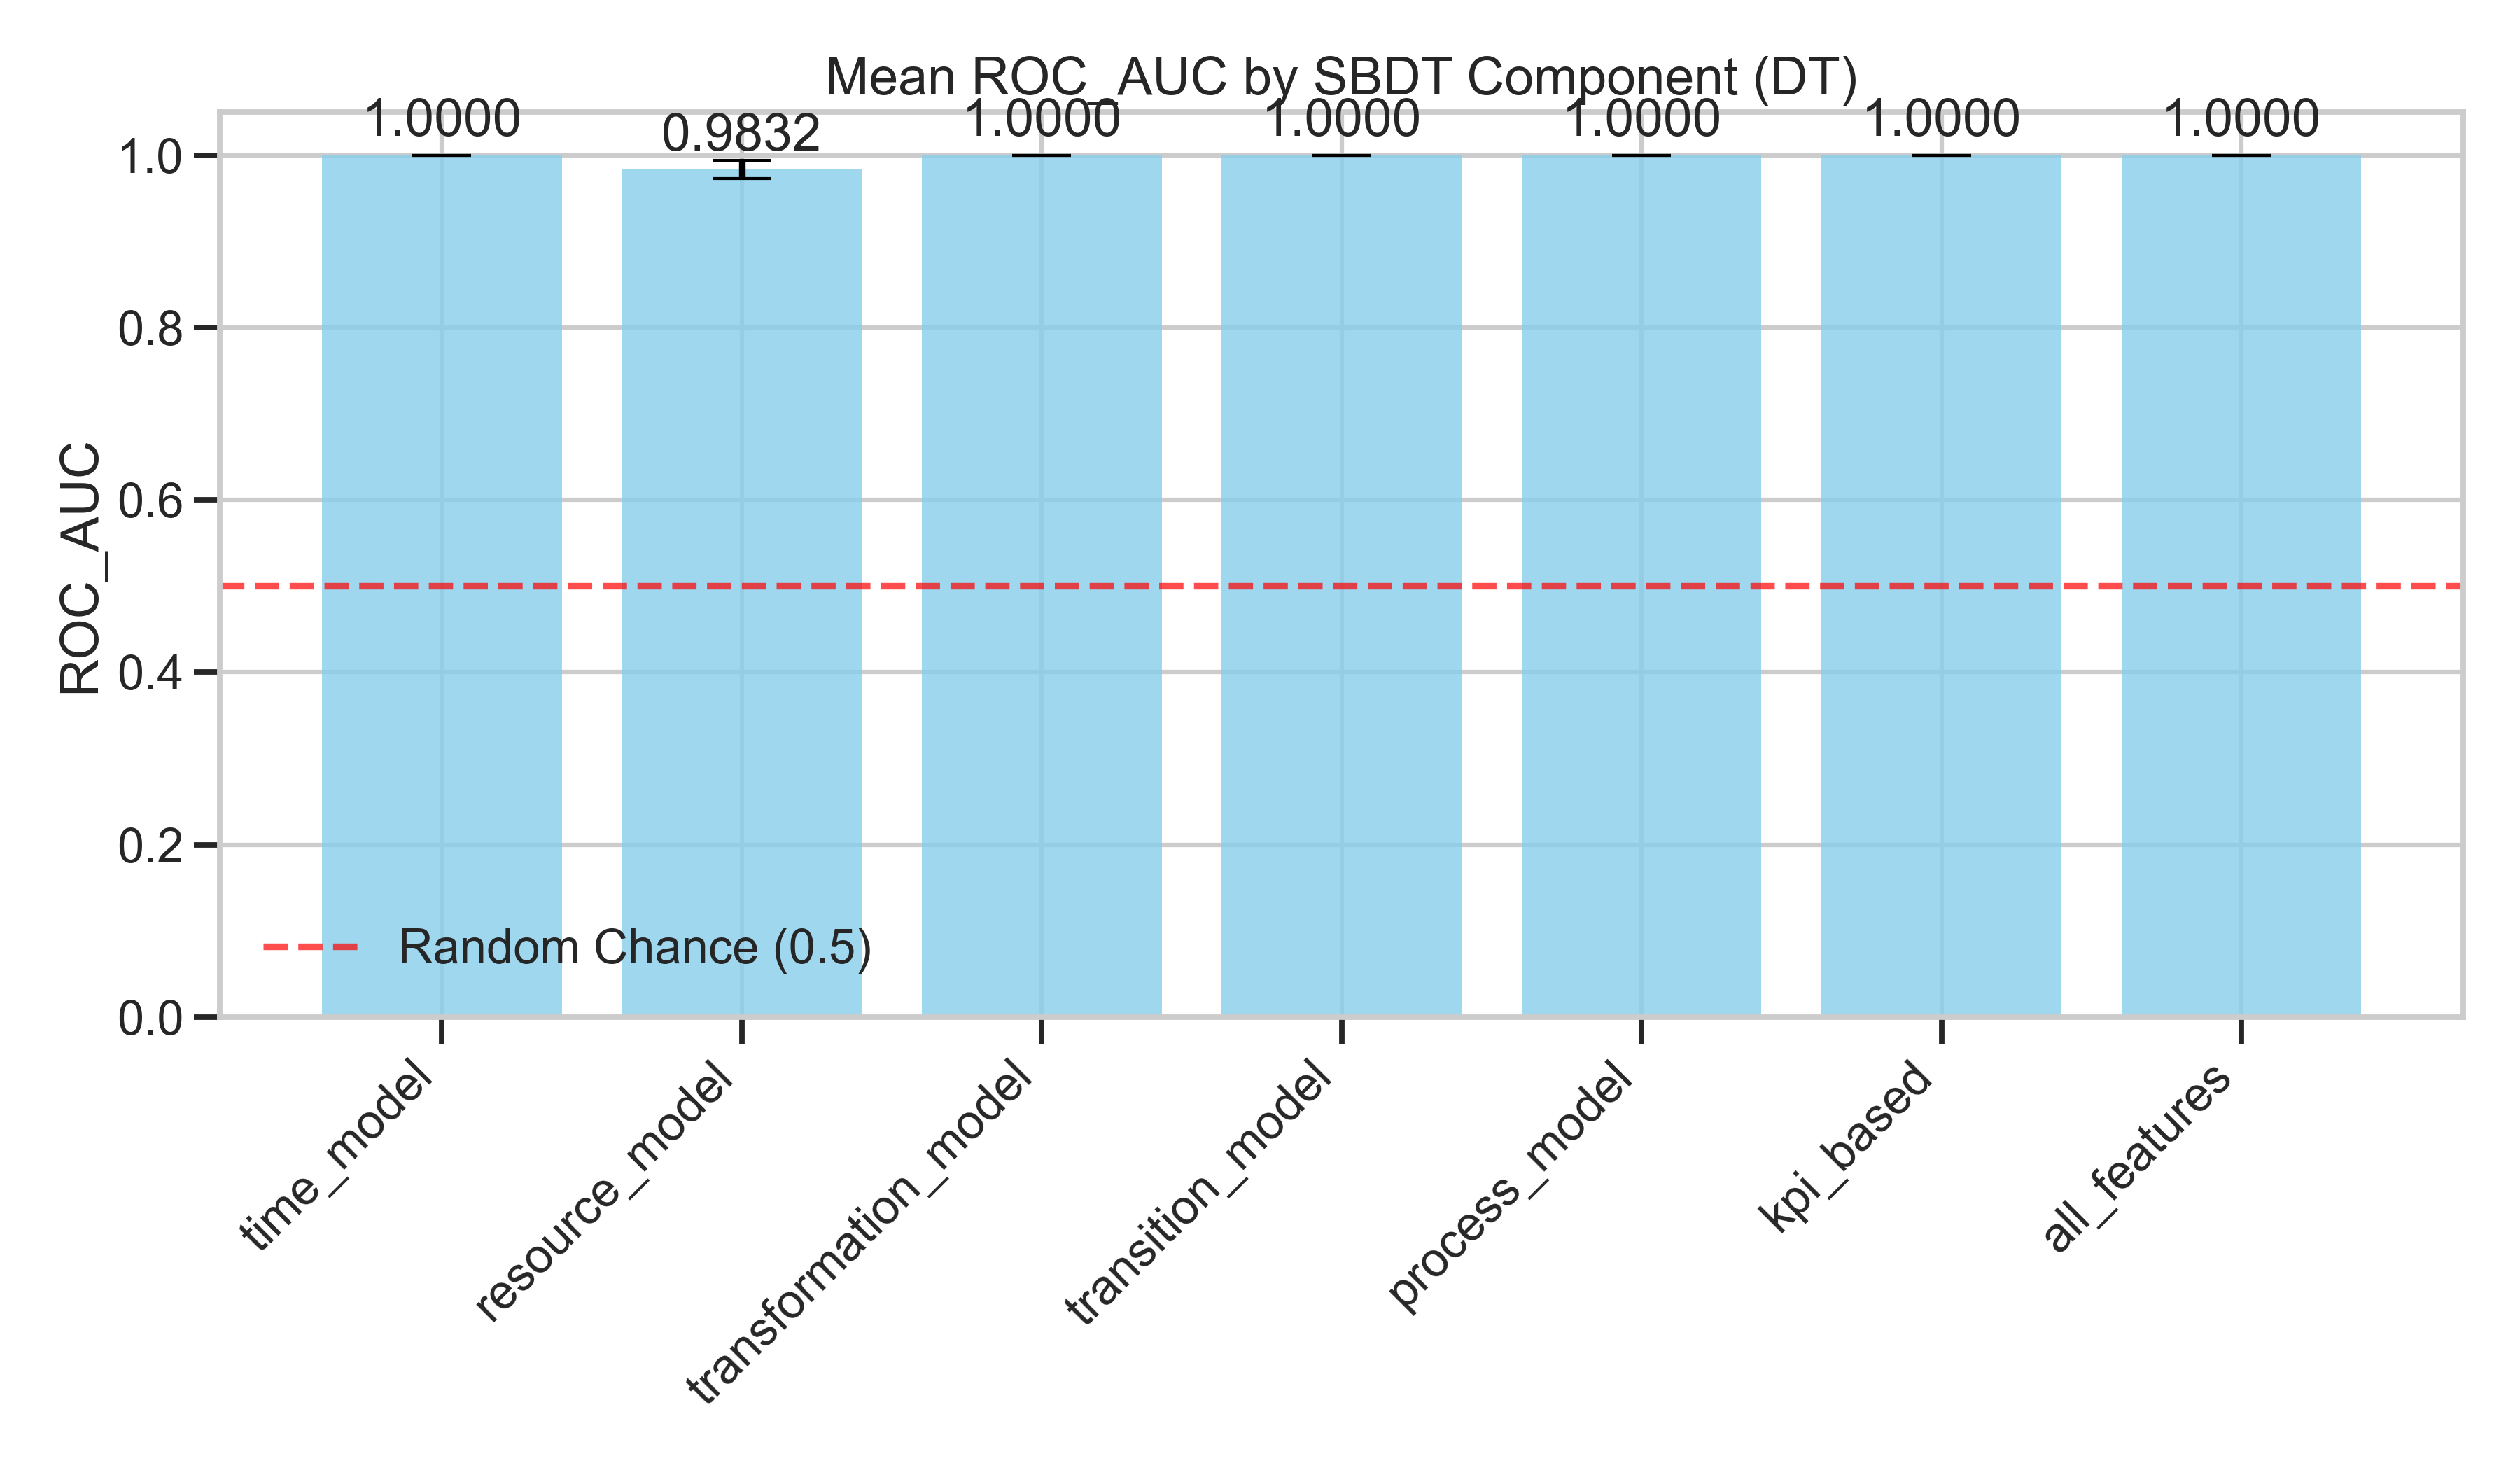
\includegraphics[width=0.8\textwidth]{figures/dt-roc-auc-by-component.png}
  \caption[Results Decision Tree]{Mean ROC AUC scores achieved by the DTree classifier when distinguishing between real and simulated data, using feature subsets corresponding to different SBDT components. Scores averaged over 10 runs. The dashed red line indicates random chance (AUC = 0.5).}
  \label{fig:dt-roc-auc}
  \caption*{Source: Own illustration.}
\end{figure}

The results from the whitebox model are highly significant. For almost all feature subsets, the DTree achieved a perfect mean ROC AUC of 1.0000, with the exception of the \texttt{resource\_model} subset which scored slightly lower but still extremely high ($\bar{S}_{obs}=0.9832 \pm 0.0104$). Correspondingly, the mean p-values were effectively zero ($< 0.0001$, reported as 0.0000) and the rejection rate was 1.00 for all components across all 10 runs. This indicates that the DTree could easily and consistently distinguish the simulated data from the real data based on the features associated with every tested SBDT component. According to the interpretation framework, this implies that, from the perspective of the whitebox model, all tested SBDT components were learned inaccurately.
Given that the mean p-value for every feature subset is far below the significance level ($\bar{p} \approx 0.0000 < \alpha = 0.05$), and the rejection rate $RR$ is 1.00 for all components, it rejects the null hypothesis ($H_0$) for every tested SBDT component based on the DTree. This provides statistically significant evidence that the model can reliably distinguish between the real process data and the simulated data using the features associated with the time model, resource model, transformation model, transition model, process model, and KPI-based perspectives, as well as when using all features combined.

\textbf{The conclusion drawn solely from this whitebox analysis is therefore that the SBDT exhibits detectable discrepancies compared to the real system across all evaluated aspects. Consequently, based on the stringent criteria of the Decision Tree's ability to find differentiating patterns (even limited to $max_depth=5$), all tested components of the SBDT are deemed inaccurate.} This suggests that, at the level of detail captured by the engineered features and marked by the DTree model, the simulation does not adequately replicate the observed behaviour of the real IoT factory. The analysis with the blackbox model in the next section will explore whether a more complex model reaches similar conclusions.

\subsection*{Results of Blackbox Model}

The blackbox validation employed the BiLSTM-based classifier described earlier in the thesis. Training this model is computationally more intensive than the DTree. Therefore, while the number of permutations ($N=1000$) and runs ($n_{runs}=10$) were maintained, the label shuffling for generating the null distribution was performed only on the test set labels for efficiency, comparing against the fixed predictions of the trained model. Furthermore, a stricter significance level of $\alpha = 0.01$ was chosen for this analysis. GPU acceleration via CUDA \autocite{NVIDIA_CUDA} was utilized to manage the computational cost.

The aggregated results from the blackbox models permutation tests are summarized in \autoref{tab:results-blackbox}, based on the report generated by the testing script. The mean AUC scores are visualized in \autoref{fig:bilstm-roc-auc}.

\begin{table}[htbp]
  \centering
  \caption[Results BiLSTM]{Blackbox BiLSTM validation results across 10 runs (N=1000, $\alpha=0.01$).}
  \label{tab:results-blackbox}
  \begin{tabular}{l l l l l p{3cm}}
    \toprule
    \textbf{Component ($\mathcal{F}_c$)} & \textbf{$\overline{\text{ROC AUC}}$} & \textbf{$\sigma_{\text{ROC AUC}}$} & \textbf{$\bar{p}$-value} & \textbf{RR} & \textbf{Assessment} \\
    \midrule
    \texttt{time\_model}                 & 0.9998                               & 0.0005                             & 0.0000                   & 1.00        & INACCURATE          \\
    \texttt{resource\_model}             & 0.9087                               & 0.1618                             & 0.0492                   & 0.90        & INACCURATE          \\
    \texttt{transformation\_model}       & 0.8705                               & 0.2094                             & 0.1879                   & 0.80        & INACCURATE          \\
    \texttt{transition\_model}           & 1.0000                               & 0.0000                             & 0.0000                   & 1.00        & INACCURATE          \\
    \texttt{process\_model}              & 0.9788                               & 0.0635                             & 0.0000                   & 1.00        & INACCURATE          \\
    \texttt{kpi\_based}                  & 0.9989                               & 0.0019                             & 0.0000                   & 1.00        & INACCURATE          \\
    \texttt{all\_features}               & 1.0000                               & 0.0000                             & 0.0000                   & 1.00        & INACCURATE          \\
    \bottomrule
  \end{tabular}
  \caption*{Source: Own tabulation.}
\end{table}

\begin{figure}[htbp]
  \centering
  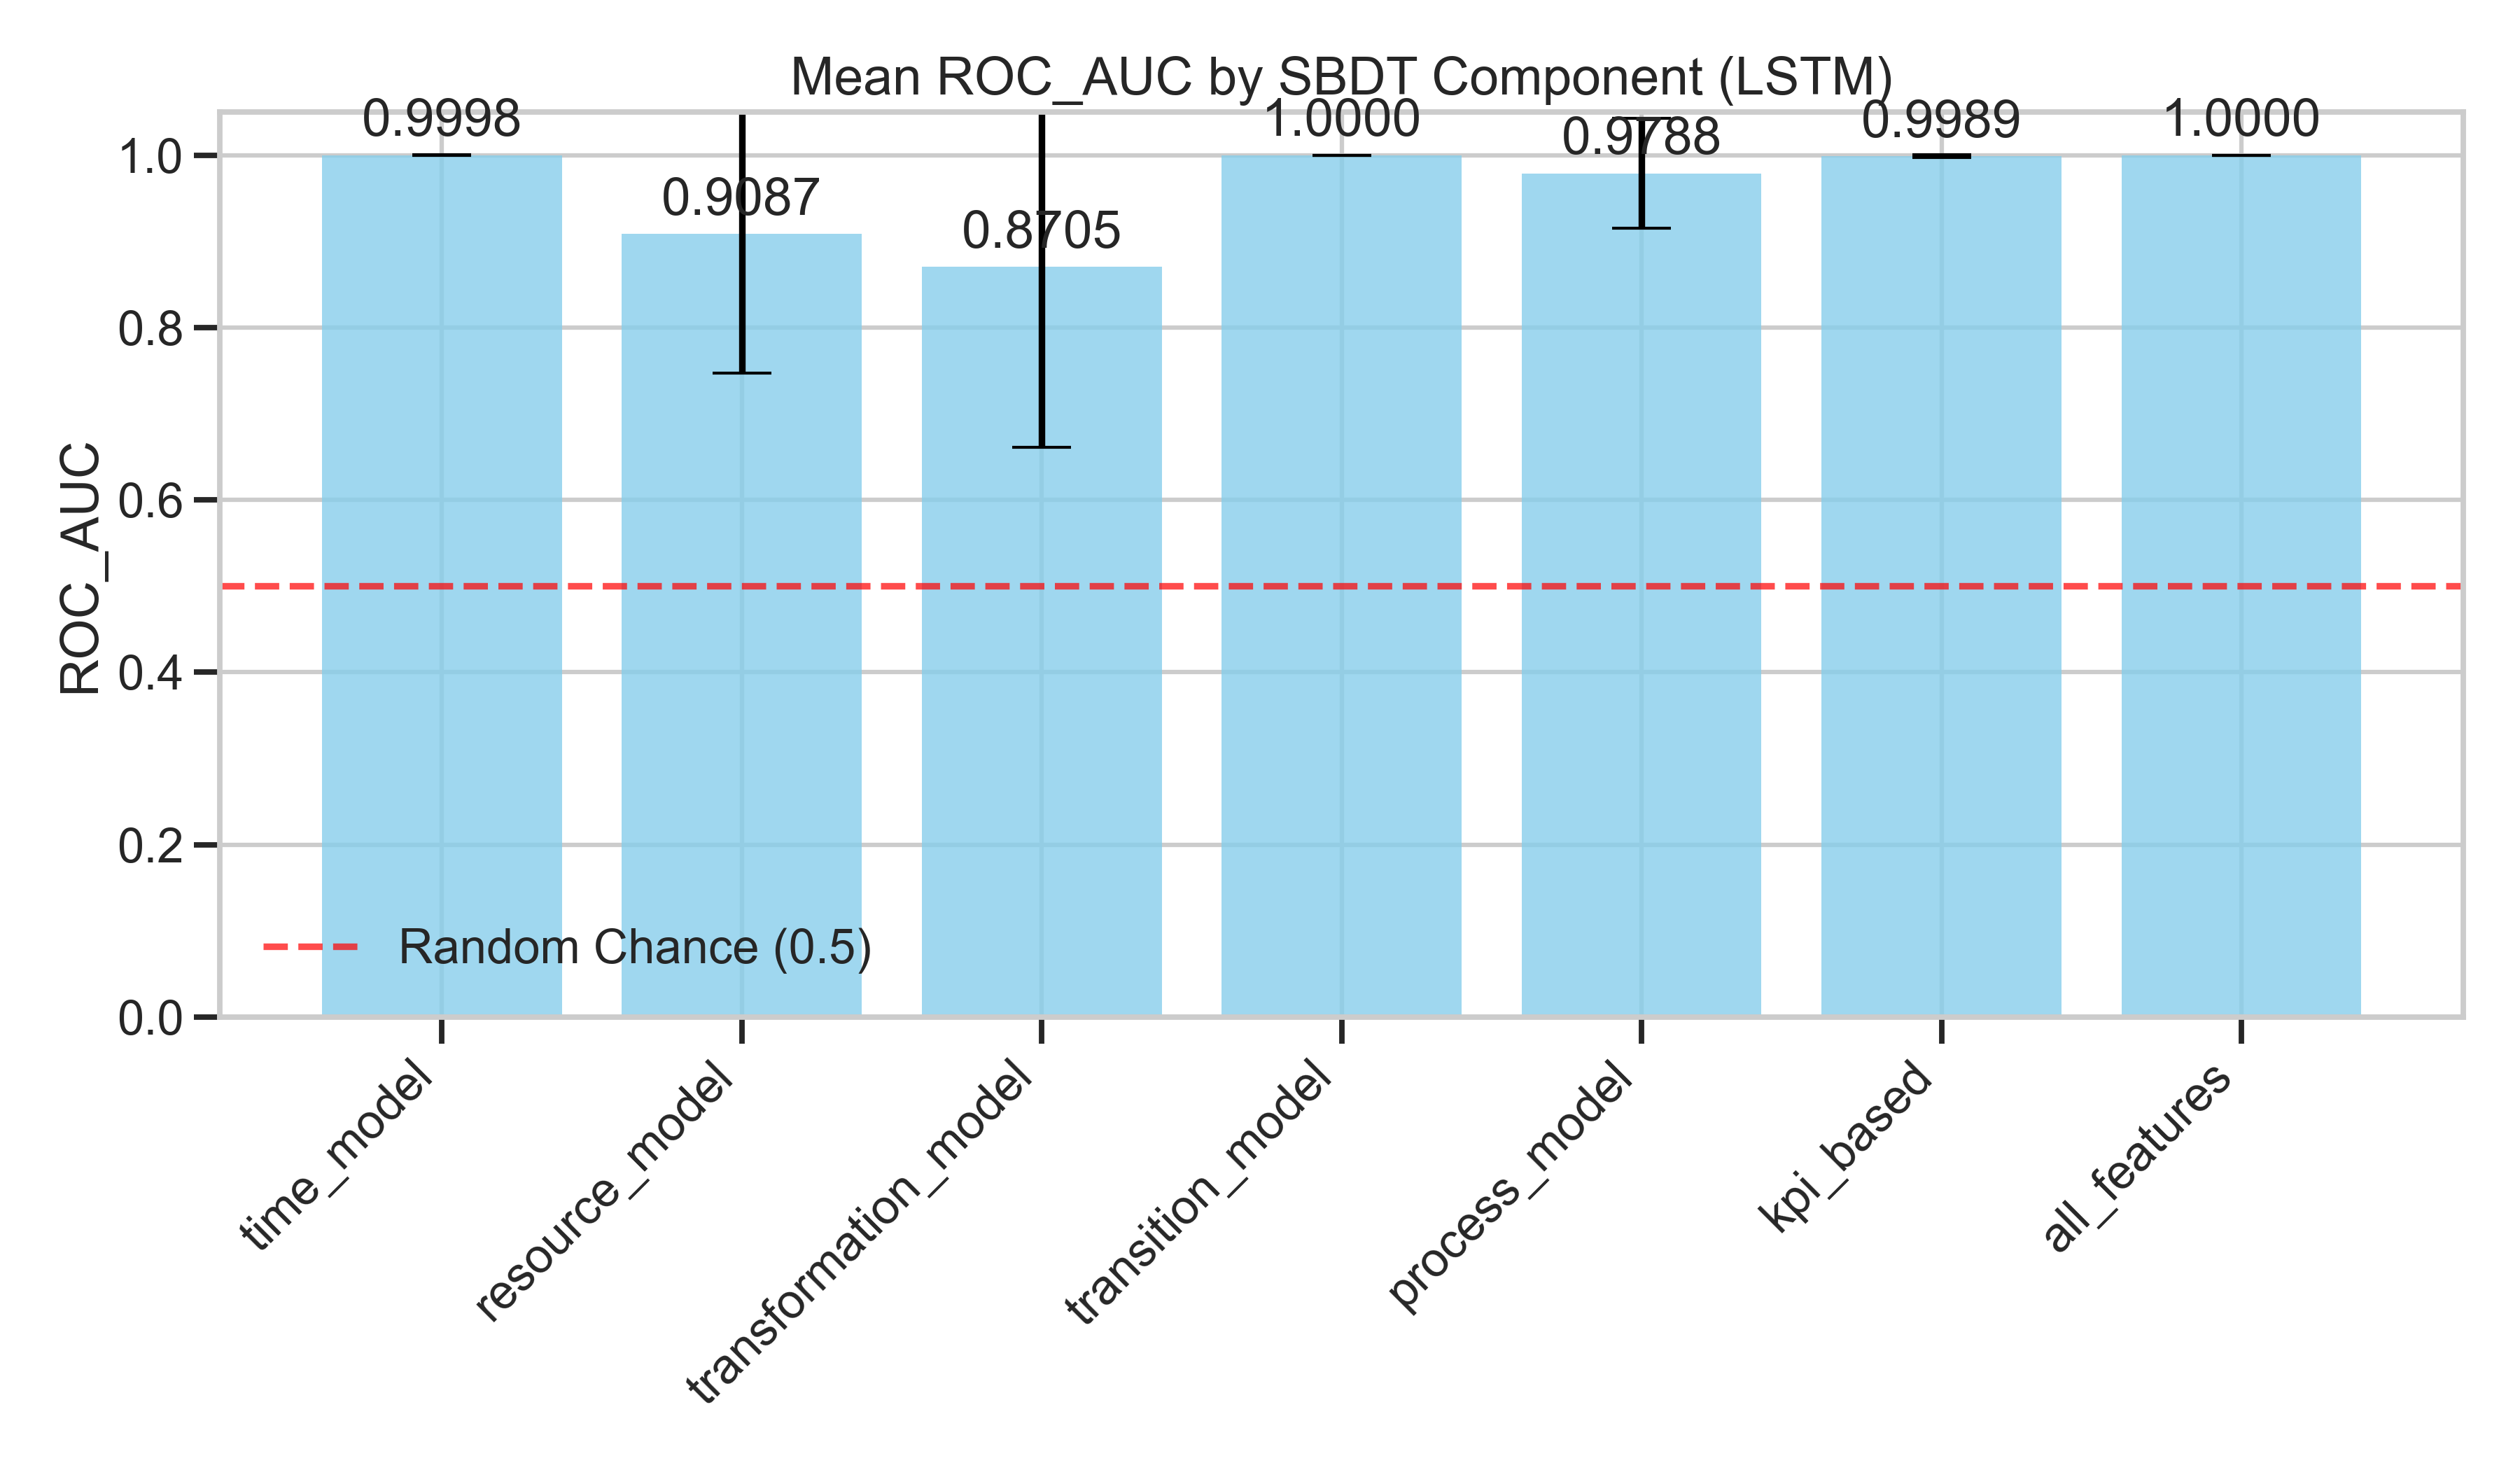
\includegraphics[width=0.8\textwidth]{figures/lstm-roc-auc-by-component.png}
  \caption[Results Blackbox model]{Mean ROC AUC scores achieved by the classifier when distinguishing between real and simulated data, using feature subsets corresponding to different SBDT components. Scores averaged over 10 runs. The dashed red line indicates random chance (AUC = 0.5).}
  \label{fig:bilstm-roc-auc}
  \caption*{Source: Own illustration.}
\end{figure}

The blackbox model results largely align with the whitebox findings, indicating significant discrepancies between the simulated and real data across various SBDT components. The BiLSTM classifier achieved very high mean ROC AUC scores for most feature subsets, particularly for \texttt{time\_model} (0.9998), \texttt{transition\_model} (1.0000), \texttt{process\_model} (0.9788), \texttt{kpi\_based} (0.9989), and \texttt{all\_features} (1.0000). For these components, the mean p-values were effectively zero, and the rejection rate $RR$ was 1.00, strongly indicating rejection of the null hypothesis ($H_0$) at the $\alpha = 0.01$ significance level.

For the \texttt{resource\_model} and \texttt{transformation\_model}, the mean ROC AUC scores were lower ($\bar{S}_{obs}=0.9087$ and $0.8705$, respectively) and exhibited considerably higher standard deviations ($\sigma_{S_{obs}}=0.1618$ and $0.2094$), suggesting greater variability in the models ability to distinguish data based on these features across the 10 runs. \textbf{Notably, while the \textit{mean} p-values (0.0492 and 0.1879) across the 10 runs were above the strict $\alpha=0.01$ threshold for these two components, $RR$ (showing the consistency of rejecting $H_0$ in individual runs) was considered the more decisive metric for the overall assessment in this multi-run framework.} The $RR$ values remained very high ($RR=0.90$ for \texttt{resource\_model}, $RR=0.80$ for \texttt{transformation\_model}). \textbf{Crucially,} a rejection rate of $0.90$ means that in 9 out of the 10 independent runs, the calculated p-value was less than the strict $\alpha=0.01$, leading to the rejection of $H_0$. Similarly, for the transformation model, $H_0$ was rejected in 8 out of 10 runs. \textbf{Therefore,} the high rejection rates across multiple runs provide strong \textbf{statistical evidence} that the BiLSTM could consistently distinguish the data \textbf{for these components as well}, supporting the rejection of $H_0$ \textbf{based on repeated testing, even considering the variability observed and the average p-value.}

\textbf{Consequently, prioritizing $RR$ which reflects statistical significance across the majority of independent runs over the potentially variable average p-value}, the analysis concludes that the blackbox model finds statistically significant differences between the real and simulated data for all tested aspects.

Similar to the whitebox analysis, the conclusion drawn from the blackbox model is \textbf{that the SBDT exhibits detectable inaccuracies compared to the real system across all evaluated components. The combination of high ROC AUC scores and, critically, the high rejection rates (RR $\ge$ 0.80 for all components) under permutation testing provide robust evidence against the null hypothesis ($H_0$) for every component. Consequently, based on the BiLSTM classifier's consistent ability to distinguish the data across multiple runs, all tested components of the SBDT are assessed as inaccurate.} This supports the finding that the current SBDT configuration, as evaluated through the engineered features, does not sufficiently replicate the behavior observed in the real IoT factory dataset.

\section{Sanity Check}
\label{sec:sanity-check}

Given the high, near-perfect ROC AUC scores observed in the main experiments (\autoref{tab:results-whitebox}, \autoref{tab:results-blackbox}), this control experiment was performed to rule out the possibility that these scores resulted from data artifacts rather than genuine SBDT fidelity issues. This 'Identical Data Control Experiment" tests if classifiers can distinguish between identical datasets solely based on assigned labels ($y=1$ versus $y=0$), using the same methodology as the main experiments but on duplicated real and simulated data separately \autocite{adebayo2018sanity}.

The results are summarized in \autoref{tab:sanity-check-results}.

\begin{table}[htbp]
  \centering
  \caption[Sanity Check]{Results of Identical Data Control Experiments (Mean ROC AUC over 10 runs)}
  \label{tab:sanity-check-results}
  \resizebox{\textwidth}{!}{%
    \begin{tabular}{l l c c c c}
      \toprule
      \textbf{Classifier} & \textbf{Feature Set ($\mathcal{F}_c$)} & \textbf{Original AUC}   & \textbf{Identical Real Data AUC} & \textbf{Identical Simulated Data AUC} & \textbf{Expected AUC}    \\
                          &                                        & \textbf{(Real vs. Sim)} & \textbf{(Real vs. Real-Copy)}    & \textbf{(Sim vs. Sim-Copy)}           & \textbf{(Random Chance)} \\
      \midrule
      Decision Tree       & \texttt{time\_model}                   & 1.0000                  & 0.3302                           & 0.3545                                & $\approx 0.5$            \\
      Decision Tree       & \texttt{resource\_model}               & 0.9832                  & 0.3916                           & 0.4140                                & $\approx 0.5$            \\
      Decision Tree       & \texttt{transformation\_model}         & 1.0000                  & 0.3903                           & 0.4072                                & $\approx 0.5$            \\
      Decision Tree       & \texttt{transition\_model}             & 1.0000                  & 0.3389                           & 0.4079                                & $\approx 0.5$            \\
      Decision Tree       & \texttt{process\_model}                & 1.0000                  & 0.3279                           & 0.4107                                & $\approx 0.5$            \\
      Decision Tree       & \texttt{kpi\_based}                    & 1.0000                  & 0.3278                           & 0.3788                                & $\approx 0.5$            \\
      Decision Tree       & \texttt{all\_features}                 & 1.0000                  & 0.3471                           & 0.3763                                & $\approx 0.5$            \\
      \midrule
      BiLSTM              & \texttt{time\_model}                   & 0.9998                  & 0.4992                           & 0.5008                                & $\approx 0.5$            \\
      BiLSTM              & \texttt{resource\_model}               & 0.9087                  & 0.4989                           & 0.5003                                & $\approx 0.5$            \\
      BiLSTM              & \texttt{transformation\_model}         & 0.8705                  & 0.5015                           & 0.4980                                & $\approx 0.5$            \\
      BiLSTM              & \texttt{transition\_model}             & 1.0000                  & 0.4998                           & 0.5007                                & $\approx 0.5$            \\
      BiLSTM              & \texttt{process\_model}                & 0.9788                  & 0.4752                           & 0.4977                                & $\approx 0.5$            \\
      BiLSTM              & \texttt{kpi\_based}                    & 0.9989                  & 0.4938                           & 0.5027                                & $\approx 0.5$            \\
      BiLSTM              & \texttt{all\_features}                 & 1.0000                  & 0.5000                           & 0.5000                                & $\approx 0.5$            \\
      \bottomrule
    \end{tabular}%
  }
  \caption*{Source: Own tabulation, incorporating results from provided summary and \autoref{tab:results-whitebox}, \autoref{tab:results-blackbox}.}
\end{table}

As shown, both classifiers achieved ROC AUC scores near the random chance baseline of 0.5 when tested on identical data in contrast to the near-perfect scores achieved on the original real vs. simulated data comparison.
This successful outcome strongly suggests the original high AUC scores were not primarily driven by artifacts. It validates the framework's core interpretation: the classifiers detected genuine, statistically significant differences between the real and simulated data. Therefore, the high AUC and RR values reported in \autoref{tab:results-whitebox} and \autoref{tab:results-blackbox} can be confidently interpreted as indicators of lower fidelity in the corresponding SBDT components, providing a reliable basis for identifying areas for model improvement.

To conclude, this chapter empirically validated the proposed VVUQ framework using the IoT Factory case study (\autoref{sec:factory}, \autoref{sec:automated-digital-twin}). The machine learning-based approach, employing both Decision Tree and BiLSTM classifiers with permutation testing (\autoref{sec:model-logic}), successfully identified statistically significant discrepancies between the SBDT and real-world data across all tested components (\autoref{tab:results-whitebox}, \autoref{tab:results-blackbox}). Crucially, identical data control experiments (\autoref{sec:sanity-check}) confirmed these findings were not due to artifacts (\autoref{tab:sanity-check-results}). The validation demonstrated the frameworks effectiveness in automatically assessing SBDT fidelity and providing component-specific feedback for improvement.
\chapter{Discussion}
\label{chap:discussion}

This chapter critically examines the findings from the empirical validation of the framework presented in \autoref{chap:case-study}, connecting these results to the broader theoretical foundations established earlier in the thesis, see \autoref{chap:theory}. The IoT Factory case study provided valuable insights into the effectiveness of the machine learning-based approach to VVUQ of simulation-based digital twins, revealing both strengths and limitations of the proposed methodology.

\section{Comparison with Traditional VVUQ Methods}
\label{sec:comparison_manual}

Traditional VVUQ practices, as discussed earlier, distinguish between verification (ensuring the model is built correctly according to specifications) and validation (ensuring the model is an accurate representation of the real system for the intended purpose). Key techniques mentioned included code inspection, debugging, unit tests, statistical tests and sensitivity analysis, see \autoref{sec:ml-approaches}. While essential, applying these techniques comprehensively to complex SBDTs faces several challenges, also highlighted previously.

The proposed ML-based validation framework, utilizing classifiers and permutation testing on event log data, primarily addresses the *validation* aspect by comparing the dynamic behaviour reflected in simulated outputs against real-world operational data. It aims to overcome some of the traditional challenges:

\begin{itemize}
  \item \textbf{Effort and Scalability:} Traditional validation relying on extensive expert consultation, manual log comparison implicit in some forms of historical data comparison, or setting up numerous simple experiments is often highly labour-intensive, see \autoref{sec:problem}. This manual effort negates some efficiency gains expected from SBDTs, especially if they are automatically generated or frequently updated. The ML approach, while requiring initial setup (data pipeline, feature engineering, model training), automates the core comparison task. Re-running the validation on new data or model versions requires mainly computational resources, addressing the identified key challenge scaling challenge better than manual review which is hard to scale up.

  \item \textbf{Scope, Depth, and Objectivity:} Comparing aggregate KPIs via statistical tests or assessing face validity through expert consultation may fail to capture subtle discrepancies in process dynamics or interactions within the SBDT. The ML approach analyses event data (\autoref{sec:data-pipeline}) and potentially complex feature interactions (\autoref{sec:feature-engineering}), offering a deeper probe into the models dynamic fidelity. The whitebox results (\autoref{sec:results-whitebox}), where the DTree identified statistically significant discrepancies (RR=1.00) across all components based on diverse feature sets, provide empirical evidence (\autoref{sec:results-whitebox}) for this potential depth. Furthermore, the use of permutation testing (\autoref{sec:permtest}) yields objective p-values, contrasting with the subjectivity inherent in expert consultation.

  \item \textbf{Applicability to Black-Box Models:} Techniques like code inspection are difficult for complex simulation platforms. The ML-based approach treats the SBDT primarily as a generator of output data. As long as comparable event logs can be extracted from the simulation and the real system, the validation method can be applied, mitigating the challenge of limited applicability to black-box models.

  \item \textbf{Continuous Validation:} Manual validation activities are often performed periodically. The automated nature of the ML pipeline lents itself better to more frequent or even continuous validation as new real-world data becomes available or the SBDT is updated, addressing a key limitation of traditional batch validation processes.

  \item \textbf{Integration:} While integrating any V\&V process presents challenges, embedding an automated data pipeline and ML testing framework might face different integration challenges compared to scheduling manual reviews or setting up traditional statistical reporting. However, once integrated, it can potentially offer more seamless feedback.
\end{itemize}

It is crucial to note that the proposed ML-based validation method primarily focuses on assessing the SBDT's fidelity against real-world data (validation). It does not replace the need for traditional \textit{verification} techniques. Methods like code inspection, unit testing, and debugging remain essential for ensuring that the simulation model itself is implemented correctly and is free from bugs. Verification ensures the model is logically correct while the ML-based validation helps determine if it is the right model relative to observed reality.

\section{Discussion in Context of Research Questions}
\label{sec:discussion_rqs}
The subsequent discussion evaluates the extent to which this objective was met by critically analysing the results of the case study (\autoref{chap:case-study}) in the context of the research questions posed in \autoref{chap:introduction}:
\begin{itemize}
  \item \textbf{RQ1:} How can automated validation and verification processes for DTs be efficiently implemented to maintain accuracy?
  \item \textbf{RQ2:} Which data-driven approaches are best suited to identify discrepancies between simulated behaviour and real operational data in discrete material flow systems?
  \item \textbf{RQ3:} To what extent does the developed framework improve the quality and reliability of DTs compared to traditional V\&V methods?
\end{itemize}

\subsection{RQ1: Efficiency of Automated VVUQ Implementation}
\label{sec:discussion_rq1}
The practical efficiency of the given VVUQ framework largely depends on the given data quality, system architecture and modelling choices. In the specific IoT Factory use case, data was readily available and documented. In companies which are not data-driven or where gathering data is difficult, this framework might need time to be created and implemented. The data pipeline needed a lot of fine tuning and data expertise for it to work. Removing processes, false entries, and other data issues took a lot of time. The setup effort was significantly higher than the execution effort of the model. Once the data pipeline was established, model training and inference was not time consuming. The largest amount of time was consumed in creating the hypothesis testing framework and assessing model quality. Referring back to the goal conflicts \autoref{fig:goals} in \autoref{sec:relevant-kpis}, the framework was able to fulfil the scalability requirements with relatively moderate computational costs and accuracy. Regarding the key challenges and requirements laid out in \autoref{sec:requirements-automatically-generated-models}, the problems of UQ and dynamic model adaption can be solved through the blackbox model. The p-values offer a quantitative measurement for UQ, while it is able to process online data (dynamic adaption). Model opacity was a trade-off with the BiLSMT structure, but may be solved if the modeller chooses the whitebox model. The key challenge of data dependency persists. During the development phase, nearly 50 hours were invested in creating the data pipeline and preprocessing.

To conclude and refer to \autoref{par:rq1} (also depicted above), the framework tackles the key challenges by providing two models that can be used based on validation goals. The whitebox model is able to provide a high level of interpretability and transparency, while the blackbox model is able to process large amounts of data and adapt to changing data. The effort of \textit{verification} still has to be carried out manually. Regarding the outlined \autoref{par:key-requirements}, the given framework is interpretable through the hypothesis testing and AFS as well as the whitebox model, integratable, scalable and can be continuously validated. The key requirement of upholding data quality was not met, as a lot of effort has been spent on manual implementation and debugging. The two-fold model approach is able to provide a good trade-off between interpretability vs. performance/accuracy. The framework balances the outlined goals, but the data quality and data dependency are still key challenges that need to be addressed.

\subsection{RQ2: Suitability of Data-Driven Approaches for Discrepancy Detection}
\label{sec:discussion_rq2}
A lot of work has been done on data-driven VVUQ approaches for all kinds of models, see \autoref{fig:pchart_knn_dt} for example. The model choice of DTree and BiLSTM seemed arbitrary and inappropriate at first, but the quantitative results indicate that both models complement each other nicely by weighing out the weaknesses of the counterpart. The DTree was not able to capture the sequential patterns in the data quite well, as it splits the data into different branches. The BiLSTM on the other side interpreted the processes with a sequence length of $19$ bidirectionally (past and future) and thus offers deeper insights. The OCEL format developed was able to capture complex dependencies in the data as it is able to store the data in a hierarchical structure and to model AND or OR processes. Different views on the processes are possible because of its object-centricness. Feature engineering highly improved the fitting of a discriminant rule of the DTree and increased the performance of the BiLSTM as well. During the engineering phase, the whitebox model can be plotted \footnote{Scikit-Learn provides a method \texttt{plot\_tree} which takes the DTree object and plots its decision rules} and the feature importance can be calculated. The feature importance of the DTree was able to show which features were important for the model and thus helped to understand the model better. It also facilitated the design of the BiLSTM architecture by showing that temporal features regarding the time model and KPIs were the best features to split the data. The DTree can thus be used as a VV tool by itself during the construction phase of the blackbox model by iteratively checking feature importances and its decision rules. This highly data-driven approach is a valuable tool for the modeller to perform a kind of sequential feature selection during feature engineering \autocite{pudil1994floating}. By iteratively adding or removing features, AFS can be performed. Also, it performed as a debugging tool. For example, complete gini impurity could be achieved between the two classes by splitting the data for an order date, an artificial value for the KPI throughput, or processes with ID $\le 27$ which were not present in the simulated data. This indicates that the model was able to detect a bug in the simulation model. The BiLSTM on the other side was of course able to utilize these splits, but is opaque. A solution can be the application of SHAP or LIME.

DTree and BiLSTM both served as appropriate choices for a data-driven VVUQ framework for SBDTs. Permutation testing complements the framework by providing a statistical significance test for the model. The p-values are able to quantify the uncertainty of the prediction. Permutation testing is particularly useful here because the underlying distribution of the OCEL and decision boundaries are unknown and had to be approximated. It was thus perfectly suited for the given data complexity. For non-sequential data, the DTree might be sufficient for VVUQ. Using a whitebox model made it easier to debug and to perform VVUQ. OCED was a suitable data structure to capture the patterns in the data. While some information might not be translatable into the OCEL standard, it serves as a good starting point for modelling efforts. Later on, the framework can be enhanced.


\subsection{RQ3: Improvement Compared to Traditional Methods}
\label{sec:discussion_rq3}

Mainly the validation process improves when using automated VVUQ approaches. The framework is able to ingest and process more information than domain experts. This offers a more comprehensive analysis than traditional checks focusing on aggregate KPIs or limited manual comparisons. The use of permutation testing (\autoref{sec:model-logic}) provides quantitative, objective measures of model fidelity, contrasting with potentially subjective traditional assessments like face validity. Furthermore, the automated nature of the validation execution addresses scalability issues common in manual methods (\autoref{sec:comparison_manual}). However, this framework primarily enhances validation and supports rather than replaces essential verification techniques outlined in traditional approaches (\autoref{sec:comparison_manual}). While it effectively identifies that discrepancies exist, root cause analysis may require further investigation, and the initial setup effort (\autoref{sec:discussion_rq1}) must be acknowledged.

In essence, the framework offers significant advancements in validation effectiveness, providing targeted, data-driven feedback to improve SBDT quality and reliability, particularly when integrated alongside traditional verification practices. AFS offers insights in which model component may be underrepresented in the SBDT and thus needs to be improved.

\section{Implications of the Findings}
\label{sec:discussion_implications}

The findings from this research carry several implications for both the theory and practice of developing and validating SBDTs, particularly those generated automatically.

\subsection{Methodological and Theoretical Insights}
\label{sec:implications_theoretical}

This work contributes to the evolving field of VVUQ for complex simulation models and DTs. The successful use of a simplified OCEL format (\autoref{tab:exemplary-ocel}) demonstrates its potential beyond PM as a structure for validation data, proving effective for feature engineering and model input despite not fully adhering to the OCED standard (\autoref{sec:object-centric-event-logs}). The core theoretical contribution lies in the novel validation paradigm proposed and tested: a supervised classification approach where simulated and real data are distinctly labelled. In contrast to unsupervised methods measuring discrepancy magnitude, like the p-charts used by \textcite{dos2024simulation}, this framework trains a classifier to distinguish the two data sources. The innovation is the reversed interpretation of its performance (\autoref{sec:discussion_rq2}): Low classifier accuracy (for example AUC $\le 0.5$) means high SBDT fidelity for the tested component relative to the feature subset, as the distributions are indistinguishable. Conversely, high accuracy indicates low fidelity\textemdash the twin failed to replicate the real complexity, making the distributions easily separable, leading to the rejection of the null hypothesis ($H_0$). This counter-intuitive interpretation, where high performance signals an inaccurately learned component, underpins the framework. It assumes that a valuable SBDT should mirror complex data patterns, more than simpler abstractions like DM or DS. While any virtual model is an abstraction, the primary abstraction considered here is the OCEL format, which is assumed to be sufficiently complete for encoding reality in this context. Furthermore, the integration of permutation testing provides statistical rigor, yielding p-values and rejection rates $RR$ that quantify the confidence in the validation assessment and offer inherent UQ. Hyperparameters $N$ (permutation count) and $\alpha$ (significance) allow tuning the VVUQ process to specific domain needs, enabling stricter thresholds where required (e.g., healthcare). This component-based fidelity assessment using AFS provides more actionable feedback than simple static scores.

Overall, this framework refines V\&V theory for automated SBDTs by changing focus from code verification to validating emergent behaviour against data distributions, demonstrating the feasibility of the layered conceptual model (\autoref{fig:framework}) developed in \autoref{chap:methodology} through its implementation (\autoref{chap:implementation}).

\subsection{Recommendations for Practical Application}
\label{sec:implications_practical}

The findings translate into several recommendations for practitioners. Firstly, prioritizing data infrastructure and quality is paramount. Implementing automated ML-based validation requires robust data pipelines, standardized formats like OCEL, and rigorous quality checks (\autoref{sec:requirements-automatically-generated-models}), as significant setup effort may be involved (\autoref{sec:discussion_rq1}). Secondly, leveraging domain knowledge remains crucial for effective feature engineering (\autoref{sec:feature-engineering}) to capture relevant process aspects aligned with SBDT components (\autoref{sec:comparing-dmfs}). Thirdly, employing a hybrid model approach is advisable: Use interpretable whitebox models like DTree for initial insights, debugging, and guiding feature selection (\autoref{sec:discussion_rq2}), supplemented by more complex blackbox models to potentially capture more intricate dynamics. Fourthly, utilize the objective fidelity metrics derived from the classification approach and permutation testing (ROC AUC, p-value, RR) (\autoref{chap:case-study}}) to enhance trust and credibility over subjective assessments (\autoref{sec:conclusion_remarks}). Fifthly, adopt component-wise validation using relevant feature subsets to gain targeted feedback for SBDT improvement. Sixthly, plan for integration with existing manufacturing systems (MES, PPC, SCADA), leveraging the framework's modular design and standard protocols (\autoref{sec:requirements-automatically-generated-models}) to enable continuous validation cycles. Finally, remember to complement this automated validation framework with traditional verification techniques (code review, unit testing) to ensure the SBDT is implemented correctly (\autoref{sec:comparison_manual}). Adopting these practices can increase the trustworthiness and utility of SBDTs in manufacturing operations.

\section{Limitations of the Study}
\label{sec:discussion_limitations}

Despite promising results, this study has limitations. Generalizability is constrained by the single case study context. The IoT Factory (\autoref{sec:factory}) using the OFacT platform (\autoref{sec:automated-digital-twin}) is a laboratory framework designed for students to assess their work. Results may differ in other domains or with other SBDT tools. Data dependency is significant as well. The framework requires quality data, and the substantial preprocessing effort noted (\autoref{sec:discussion_rq1}, \autoref{sec:data-pipeline}), including filling missing values with zeros (\autoref{sec:factory}), presents a practical challenge and potential point of influence on results. Methodological choices, such as the specific classifiers (DTree vs. BiLSTM), engineered features (\autoref{sec:feature-engineering}), and permutation test parameters (N, $\alpha$) (\autoref{tab:results-whitebox}, \autoref{tab:results-blackbox}), impact outcomes and represent specific points in a larger design space. The scope of VVUQ is primarily focused on automated validation via behavioural comparison. Formal verification and detailed UQ are not covered.

A key aspect is that manual verification remains the main limitation of this framework. Furthermore, interpretability of discrepancies poses a challenge; while the framework identifies inaccurate components (\autoref{sec:discussion_rq2}), determining the root cause, especially with the BiLSTM, requires further investigation, potentially using XAI tools or expert analysis. Lastly, the reliance on a simplified OCEL format means the validation is performed on an abstraction of reality (\autoref{sec:conclusion_summary_findings}); detected differences could partially reflect format limitations, or the format might obscure other discrepancies.

\section{Discussion Summary}
\label{sec:discussion_summary}

In summary, this chapter critically discussed the thesis findings, connecting the empirical results from the IoT Factory case study to the theoretical foundations. The ML-based VVUQ framework demonstrated potential for improving the validation of SBDTs. The discussion contextualized the answers to the research questions, affirming the potential for efficient implementation despite initial setup costs \autoref{par:rq1}, validating supervised classification with a novel reversed interpretation as a suitable data-driven approach \autoref{par:rq2}, and confirming improvements in validation scope, depth, and objectivity over traditional methods \autoref{par:rq3}.
\chapter{Conclusion and Future Work}
\label{chap:conclusion}

\section{Summary of Key Findings and Contributions}
\label{sec:conclusion_summary_findings}

This thesis addressed the critical challenge of efficiently validating and verifying automatically generated SBDTs for DMFS. The research was guided by three core questions \autoref{sec:problem}, which this work aimed to answer:

Regarding RQ1 \autoref{par:rq1}, the study demonstrated that while significant effort at the beginning is required for data pipeline setup and feature engineering, also concerning data quality, the operational execution of the proposed VVUQ framework can be highly efficient and scalable. The framework utilizes a two-model approach (whitebox DTree and blackbox BiLSTM) to balance interpretability and performance, automating the core validation and uncertainty quantification task once established. The efficiency stems from leveraging readily available simulation and real-world data, processed into an OCEL format.

In response to RQ2 \autoref{par:rq2}, the empirical validation confirmed that data-driven supervised classification is possible for identifying discrepancies between simulated SBDT behaviour and real operational data. By labelling simulated data differently from real data, a binary classifier is trained to distinguish between them. The innovation lies in the reversed interpretation of the classifier's performance: \textit{Low} performance (AUC $\le 0.5$) implies that the SBDT component has been learned accurately relative to the tested features, as the simulated and real distributions are statistically indistinguishable. Conversely, \textit{high} classifier performance indicates that the component was \textit{not} learned accurately, as the distributions are easily separable. This contrasts with unsupervised approaches like \textcite{dos2024digital} which measure discrepancy magnitude with p-charts, and also runs counter to the intuition that high performance always signals success. Here, high performance signals high distinguishability, meaning the twin failed to replicate the complex manifold of the real data for that component. Permutation testing (\autoref{sec:model-logic}) provided a robust method for assessing the statistical significance (p-value) and consistency (Rejection Rate, $RR$) of this distinguishability. This approach makes the assumption that a successful SBDT must accurately reflect complex underlying data patterns, going further than simpler abstractions like DM or DS, and that the chosen OCEL format is suitable to encode the relevant aspects of reality.

Addressing RQ3 \autoref{par:rq3}, the developed ML framework demonstrated improvements over traditional V\&V approaches (\autoref{sec:comparison_manual}). The case study (\autoref{chap:case-study}) showed enhanced context and objectivity, systematically identifying inaccuracies across all tested SBDT components with high statistical significance (\autoref{tab:results-whitebox}, \autoref{tab:results-blackbox}). This automated VVUQ capability offers advantages in scalability and objectivity. The significance level ($\alpha$) and number of permutations ($N$) can be tuned based on domain-specific requirements (e.g., lower $\alpha$, higher $N$ in safety-critical applications like healthcare).

The main empirical results from the IoT Factory case study (\autoref{chap:case-study}) showed that both classifiers achieved high performance for most components, leading to the rejection of the null hypothesis ($H_0$) and the conclusion that these components were inaccurate in the current SBDT configuration. This highlights the frameworks sensitivity in detecting deviations and provides specific clues for targeted SBDT model improvement or recalibration

The primary contributions of this thesis are:
\begin{enumerate}
  \item The development and conceptualization of a multi-layered, automated VVUQ framework (\autoref{fig:framework}) leveraging supervised classification for SBDT fidelity assessment.
  \item A novel methodological interpretation where low classifier performance indicates high SBDT fidelity for specific components/features, combined with permutation testing for statistical rigor (validation) and uncertainty quantification (p-values, $RR$).
  \item Empirical demonstration of the frameworks ability to target inaccuracies in an industrial SBDT case study (\autoref{chap:case-study}).
\end{enumerate}

However, a \testit{main limitation} stays: The framework automates validation and uncertainty quantification but relies on \textit{manual verification} to ensure the SBDT model is built correctly according to its conceptual description and specifications.

\section{Concluding Remarks}
\label{sec:conclusion_remarks}

The increasing adoption of SBDTs necessitates robust and efficient VVUQ methods to ensure trust and reliability. Traditional approaches face significant hurdles in scalability and objectivity when applied to complex, automatically generated twins. This thesis proposed and validated a novel, data-driven framework using supervised classification with a reversed interpretation of performance metrics, complemented by permutation testing. This approach offers a scalable, objective, and statistically grounded method for assessing SBDT fidelity component-wise. The empirical success in identifying specific areas of inaccuracy underscores the value of data-driven validation. While verification remains a manual task and data quality is paramount, this work contributes a significant step towards continuous, automated, and trustworthy validation of SBDTs, essential for their successful deployment in demanding Industry 4.0 applications.

\section{Future Research Directions}
\label{sec:conclusion_future_work}

Based on the findings and limitations identified (\autoref{sec:discussion_limitations}), several avenues for future research emerge:

\begin{itemize}
  \item \textbf{Enhancing Interpretability (Root Cause Analysis):} Integrate XAI techniques (SHAP, LIME) to move beyond identifying that a component is inaccurate (high classifier performance) to explaining why, thereby facilitating targeted model correction.
  \item \textbf{Refining Uncertainty Quantification:} Further explore methods like BNNs or MCD to provide richer UQ measures beyond the p-value/RR, potentially offering confidence intervals on the fidelity assessment itself.
  \item \textbf{Automated Recalibration and Verification Support:} Develop mechanisms for automated SBDT recalibration triggered by validation results. Explore how the frameworks outputs could potentially support or partially automate aspects of manual verification, addressing the main limitation.
  \item \textbf{Improving Online Capabilities and Integration:} Enhance the framework for robust real-time operation, optimizing data stream processing and developing standardized interfaces for seamless integration into industrial IoT environments.
  \item \textbf{Addressing Data Quality and Pipeline Automation:} Research more automated techniques for ensuring input data quality and streamlining the data pipeline setup, potentially leveraging AutoML or anomaly detection on the input data itself.
  \item \textbf{Investigating Foundational Assumptions:} Conduct studies on the impact of the OCEL format's completeness and the assumption regarding required SBDT complexity across different application domains.
  \item \textbf{Generalizability and Broader Application:} Validate the framework's effectiveness and the reversed interpretation hypothesis across diverse industrial domains, SBDT platforms, and levels of system complexity.
  \item \textbf{Exploring Alternative ML Approaches:} Investigate other promising ML techniques not yet applied in this specific concurrent VVUQ context. The Local Outlier Factor (LOF), a distance-based approach, could identify outliers potentially linked to rare events or concept drift \autocite{alghushairy2020review}. Density-based methods like DBSCAN identify anomalies in low-density regions \autocite{ccelik2011anomaly}, distinguishing normal clusters from deviations. Isolation Forest offers efficiency for high-dimensional data by isolating anomalies quickly through random partitioning \autocite{xu2017improved}. One-Class SVMs \autocite{li2003improving} could be useful when only normal data is available, learning a boundary for normal operations. Autoencoders (AE) \autocite{zhou2017anomaly} trained on normal data can detect anomalies via high reconstruction errors, capturing complex non-linear patterns. Furthermore, semi-supervised techniques could leverage small amounts of labelled anomaly data alongside larger normal datasets to enhance detection.
\end{itemize}

Addressing these directions will further mature automated VVUQ methodologies, making SBDTs more reliable, trustworthy, and impactful in practice. \blacksquare
\chapter*{Eigenständigkeitserklärung}
\thispagestyle{plain}

\vspace{0.5em}

Hiermit versichere ich

\vspace{0.5em}

\noindent
\begin{tabular}{ll}
  \textbf{Name, Vorname}  & \rule{8cm}{0.4pt} \\
  \textbf{Matrikelnummer} & \rule{8cm}{0.4pt} \\
  \textbf{Studiengang}    & \rule{8cm}{0.4pt}
\end{tabular}

\vspace{1em}

\noindent
dass ich die vorliegende mit dem Thema

\begin{center}
  \large\bfseries
  Automatic Verification and Validation of Automatically Generated \\
  Simulation-Based Digital Twins for Discrete Material Flow Systems
\end{center}

\vspace{0.5em}

\noindent
selbstständig und ohne die Benutzung anderer als der angegebenen Hilfsmittel angefertigt habe. \\
Alle Stellen – einschließlich Tabellen, Karten, Abbildungen etc. –, die wörtlich oder sinngemäß aus veröffentlichten und nicht veröffentlichten Werken und Quellen (dazu zählen auch Internetquellen) entnommen wurden, sind in jedem einzelnen Fall mit exakter Quellenangabe kenntlich gemacht worden. \\

\noindent
Zusätzlich versichere ich, dass ich beim Einsatz von generativen IT-/KI-Werkzeugen (z. B. ChatGPT, BARD, Dall-E oder Stable Diffusion) diese Werkzeuge in einer Rubrik \enquote{Übersicht verwendeter Hilfsmittel} mit ihrem Produktnamen, der Zugriffsquelle (z. B. URL) und Angaben zu genutzten Funktionen der Software sowie Nutzungsumfang vollständig angeführt habe. Wörtliche sowie paraphrasierende Übernahmen aus Ergebnissen dieser Werkzeuge habe ich analog zu anderen Quellenangaben gekennzeichnet. \\


\noindent
Mir ist bekannt, dass es sich bei einem Plagiat um eine Täuschung handelt, die gemäß der Prüfungsordnung sanktioniert wird. \\



\noindent
Ich versichere, dass ich die vorliegende Arbeit oder Teile daraus nicht bereits anderweitig innerhalb oder außerhalb der Hochschule als Prüfungsleistung eingereicht habe. \\

\vspace{1.5em}

\noindent
\begin{tabular}{ll}
  Ort, Datum \rule{7cm}{0.4pt} \\[1em]
  Unterschrift \rule{7cm}{0.4pt}
\end{tabular}
\chapter*{Übersicht verwendeter Hilfsmittel}
\thispagestyle{plain}

\section*{Generative KI-Werkzeuge}

\begin{tabular}{p{3cm}p{5cm}p{7cm}}
  \textbf{Tool}   & \textbf{Zugriffsquelle}                   & \textbf{Verwendungszweck}                                                                                                                                                                                                                  \\
  \hline
  GitHub Copilot  & \url{https://github.com/features/copilot} &
  Formatierung und Einrückung von Code. Nutzung als Debugging Unterstützung für die schnellere Erkennung von Fehlern im Code. Generierung von \textbf{Dokumentationsunterlagen} wie README, Code Kommentaren und Lizenzen. Anwendung von Vorschlägen für die Architektur des Frameworks                    \\
  \hline
  ChatGPT         & \url{https://chat.openai.com}             &
  Formulierungshilfe für englische Textpassagen, Korrekturvorschläge für Grammatik, Umformulierung komplexer Sätze. Rechtschreibunterstützung. Anfertigung von mathematischen Zeichungen und PlantUML Diagrammen auf Basis von Bildern. Erstellung von Formeln in \LaTeX auf Basis von Paperinformationen. \\
  \hline
  DeepL           & \url{https://deepl.com}                   &
  Überprüfung der englischen Grammatik und Rechtschreibung im gesamten Dokument.                                                                                                                                                                                                                           \\
  \hline
  Research Rabbit & \url{https://researchrabbitapp.com/}      &
  Literaturrecherche und Management.                                                                                                                                                                                                                                                                       \\
  \hline
\end{tabular}

\section*{Verwendungsumfang}

Die generativen KI-Werkzeuge wurden wie folgt eingesetzt:

\begin{itemize}
  \item \textbf{GitHub Copilot}: Hauptsächlich zur Unterstützung bei Implementierungsdetails im Python-Code für die Datenverarbeitung und Modellierung. Alle generierten Vorschläge wurden manuell überprüft, verstanden und bei Bedarf angepasst. Verwendung in ca. 35\% der gesamten Codeimplementierung.

  \item \textbf{ChatGPT}: Zur sprachlichen Verbesserung komplexer wissenschaftlicher Formulierungen, insbesondere bei methodologischen Beschreibungen und Diskussionen. Alle Formulierungsvorschläge wurden kritisch geprüft und in den Kontext der eigenen Argumentation integriert. Unterstützung bei ca. 30\% des geschriebenen Texts.

  \item \textbf{DeepL}: Überprüfung der finalen Version auf grammatikalische und stilistische Fehler. Vorgeschlagene Korrekturen wurden manuell überprüft und nur bei Erhaltung des beabsichtigten wissenschaftlichen Inhalts übernommen.
  \item \textbf{Research Rabbit}: Unterstützung bei der Literaturrecherche und -verwaltung.
\end{itemize}

\section*{Kennzeichnung generierter Inhalte}

Alle durch KI-Werkzeuge vorgeschlagenen Formulierungen, die substantiell in den Text übernommen wurden, sind durch das Symbol \ai{Text} gekennzeichnet. Geringfügige grammatikalische oder stilistische Anpassungen wurden nicht separat markiert, da sie den Inhalt nicht wesentlich verändert haben.

Inhalte aus wissenschaftlichen Quellen und eigene Gedanken stellen den überwiegenden Teil der vorliegenden Arbeit dar. Die Verwendung generativer Werkzeuge diente ausschließlich der sprachlichen und technischen Unterstützung und hat die eigene kritische Auseinandersetzung mit dem Forschungsthema nicht ersetzt.

=========================================================================
% Appendix Section: Mathematical Foundations
% =========================================================================
\section{Mathematical Foundations}
\label{app:math_foundations}

This appendix provides formal definitions and illustrations for the core mathematical functions and operations referenced in the theoretical foundations chapter (Section~\ref{sec:rnn} onwards), as well as other relevant mathematical concepts and techniques commonly encountered in machine learning, deep learning, optimization, and data handling that are pertinent to the methods employed in this thesis. % Adjust Section ref if needed

% -------------------------------------------------------------------------
\subsection{Basic Notation and Operations}
% -------------------------------------------------------------------------
% (Content from previous version - vectors, matrices, basic ops...)
As established at the beginning of the chapter, vectors are denoted by bold lowercase letters (e.g., \( \bm{z} \)) and matrices by uppercase letters (e.g., \( W \)). Vectors are assumed to be column vectors unless otherwise specified.

\paragraph{Matrix-Vector Multiplication:}
Given a matrix \( W \in \mathbb{R}^{m \times n} \) and a vector \( \bm{x} \in \mathbb{R}^n \), their product is a vector \( \bm{y} = W\bm{x} \in \mathbb{R}^m \), where the \( i \)-th element is calculated as:
\begin{equation}
  y_i = \sum_{j=1}^{n} W_{ij} x_j
\end{equation}

\paragraph{Vector Addition:}
Given two vectors \( \bm{y}, \bm{b} \in \mathbb{R}^m \), their sum is a vector \( \bm{z} = \bm{y} + \bm{b} \in \mathbb{R}^m \), computed element-wise:
\begin{equation}
  z_i = y_i + b_i
\end{equation}

\paragraph{Element-wise (Hadamard) Product:}
Given two vectors \( \bm{a}, \bm{b} \in \mathbb{R}^m \), their Hadamard product is a vector \( \bm{c} = \bm{a} \odot \bm{b} \in \mathbb{R}^m \), computed element-wise:
\begin{equation}
  c_i = a_i \cdot b_i
\end{equation}
This operation is notably used in LSTM cells to apply gate activations (Section~\ref{sec:lstm}).

\paragraph{Vector Concatenation:}
Given two vectors \( \bm{a} \in \mathbb{R}^{d_a} \) and \( \bm{b} \in \mathbb{R}^{d_b} \), their concatenation \( \bm{c} = [\bm{a} ; \bm{b}] \) results in a vector \( \bm{c} \in \mathbb{R}^{d_a + d_b} \) formed by stacking the elements of \( \bm{b} \) below the elements of \( \bm{a} \). This is used in Bi-LSTMs (Equation~\ref{eq:bilstm_concat}) and Multi-Head Attention (Equation~\ref{eq:multihead_attention}).

\paragraph{Matrix Transpose:}
The transpose of a matrix \( A \in \mathbb{R}^{m \times n} \), denoted \( A^T \in \mathbb{R}^{n \times m} \), is obtained by swapping its rows and columns:
\begin{equation}
  (A^T)_{ij} = A_{ji}
\end{equation}
This is used in the Scaled Dot-Product Attention formula (Equation~\ref{eq:scaled_dot_product_attention}).


% -------------------------------------------------------------------------
\subsection{Activation Functions}
% -------------------------------------------------------------------------
% (Content from previous version - Sigmoid, Tanh, ReLU, Softmax with plots)
Activation functions introduce non-linearity into neural network models, allowing them to learn complex patterns. They are typically applied element-wise to the output of a linear transformation \( \bm{z} = W\bm{x} + \bm{b} \).

\paragraph{Sigmoid Function (\( \sigma \)):}
The standard sigmoid function maps any real input to the range (0, 1). It is defined as:
\begin{equation}
  \sigma(z) = \frac{1}{1 + e^{-z}}
\end{equation}
Due to its output range, it is commonly used for gating mechanisms in LSTMs (Equations~\ref{eq:lstm_forget_gate}, \ref{eq:lstm_input_gate}, \ref{eq:lstm_output_gate}) and for producing probabilities in binary classification outputs. A plot is shown in Figure~\ref{fig:sigmoid_plot}.

\begin{figure}[htbp]
  \centering
  \begin{tikzpicture}
    \begin{axis}[
        width=0.6\textwidth, % Adjust width as needed
        height=6cm,
        axis lines=middle,
        xlabel={$z$},
        ylabel={$\sigma(z)$},
        grid=major,
        ymin=-0.1, ymax=1.1,
        xmin=-6.5, xmax=6.5,
        samples=100,
        domain=-6:6,
        legend pos=outer north east % Or other position
      ]
      \addplot [blue, thick] {1/(1+exp(-x))};
      \addlegendentry{$\sigma(z) = \frac{1}{1+e^{-z}}$}
      % Asymptotes
      \addplot [dashed, gray, domain=-6.5:6.5] {0};
      \addplot [dashed, gray, domain=-6.5:6.5] {1};
    \end{axis}
  \end{tikzpicture}
  \caption{The Sigmoid activation function.}
  \label{fig:sigmoid_plot}
\end{figure}


\paragraph{Hyperbolic Tangent Function (\( \tanh \)):}
The hyperbolic tangent function maps any real input to the range (-1, 1). It is defined as:
\begin{equation}
  \tanh(z) = \frac{e^z - e^{-z}}{e^z + e^{-z}} = 2\sigma(2z) - 1
\end{equation}
It is frequently used as the main activation function for hidden states in RNNs and LSTMs (e.g., Equations~\ref{eq:rnn_hidden_state}, \ref{eq:lstm_candidate_cell}, \ref{eq:lstm_hidden_state}). See Figure~\ref{fig:tanh_plot}.

\begin{figure}[htbp]
  \centering
  \begin{tikzpicture}
    \begin{axis}[
        width=0.6\textwidth,
        height=6cm,
        axis lines=middle,
        xlabel={$z$},
        ylabel={$\tanh(z)$},
        grid=major,
        ymin=-1.2, ymax=1.2,
        xmin=-4.5, xmax=4.5,
        samples=100,
        domain=-4:4,
        legend pos=outer north east
      ]
      \addplot [red, thick] {tanh(x)};
      \addlegendentry{$\tanh(z)$}
      % Asymptotes
      \addplot [dashed, gray, domain=-4.5:4.5] {-1};
      \addplot [dashed, gray, domain=-4.5:4.5] {1};
    \end{axis}
  \end{tikzpicture}
  \caption{The Hyperbolic Tangent (tanh) activation function.}
  \label{fig:tanh_plot}
\end{figure}


\paragraph{Rectified Linear Unit (ReLU):}
The ReLU function outputs the input directly if it is positive, and zero otherwise. It is defined as:
\begin{equation}
  \text{ReLU}(z) = \max(0, z)
\end{equation}
ReLU is widely used in deep learning due to its simplicity and effectiveness in mitigating the vanishing gradient problem for positive inputs. It is used within the model presented in this thesis (Section~\ref{sec:integrated_architecture} refers to the code using it). See Figure~\ref{fig:relu_plot}.

\begin{figure}[htbp]
  \centering
  \begin{tikzpicture}
    \begin{axis}[
        width=0.6\textwidth,
        height=6cm,
        axis lines=middle,
        xlabel={$z$},
        ylabel={ReLU$(z)$},
        grid=major,
        ymin=-1, ymax=4.5,
        xmin=-4.5, xmax=4.5,
        samples=100,
        legend pos=outer north east
      ]
      \addplot [green!60!black, thick, domain=-4:4] {max(0,x)};
      \addlegendentry{ReLU$(z) = \max(0, z)$}
    \end{axis}
  \end{tikzpicture}
  \caption{The Rectified Linear Unit (ReLU) activation function.}
  \label{fig:relu_plot}
\end{figure}


\paragraph{Softmax Function:}
The softmax function converts a vector of K real numbers \( \bm{z} = (z_1, ..., z_K) \) into a probability distribution consisting of K probabilities. The function is applied to the entire vector and the \( i \)-th element of the output vector is calculated as:
\begin{equation}
  \text{softmax}(\bm{z})_i = \frac{e^{z_i}}{\sum_{j=1}^K e^{z_j}} \quad \text{for } i = 1, ..., K
\end{equation}
The outputs are non-negative and sum to 1 (\( \sum_{i=1}^K \text{softmax}(\bm{z})_i = 1 \)). Softmax is commonly used in the output layer of multi-class classification models and plays a crucial role in normalizing scores into attention weights in the Attention mechanism (Equation~\ref{eq:scaled_dot_product_attention}).

% -------------------------------------------------------------------------
\subsection{Attention Mechanism Components}
% -------------------------------------------------------------------------
% (Content from previous version - Dot Product, Scaling)
The Scaled Dot-Product Attention mechanism (Equation~\ref{eq:scaled_dot_product_attention}) relies on several fundamental operations beyond the Softmax function:

\paragraph{Dot Product Similarity:}
The compatibility between a query \( \bm{q} \) and a key \( \bm{k} \) (both typically vectors of the same dimension \( d_k \)) is often computed using the dot product \( \bm{q} \cdot \bm{k} = \bm{q}^T \bm{k} \). For matrices \( Q \) and \( K \) containing multiple queries and keys as rows, the matrix product \( QK^T \) computes all pairwise dot products efficiently.

\paragraph{Scaling:}
To counteract the effect of large dot product values when the dimension \( d_k \) is high, the scores \( QK^T \) are scaled down by dividing by \( \sqrt{d_k} \) before applying the softmax function. This helps maintain a stable gradient flow during training.

% -------------------------------------------------------------------------
\subsection{Normalization Techniques}
% -------------------------------------------------------------------------
Normalization layers help stabilize training, speed up convergence, and sometimes improve generalization by standardizing layer inputs.

\paragraph{Layer Normalization (LayerNorm):}
Layer Normalization normalizes the inputs across the features for \textit{each individual data sample} in a batch, making its computation independent of the batch size. For an input vector \( \bm{x} \) representing the features for one sample at a specific layer, LayerNorm computes:
\begin{equation}
  \text{LayerNorm}(\bm{x}) = \bm{\gamma} \odot \frac{\bm{x} - \mu_{\text{sample}}}{\sqrt{\sigma^2_{\text{sample}} + \epsilon}} + \bm{\beta}
  \label{eq:layernorm}
\end{equation}
Here, \( \mu_{\text{sample}} \) and \( \sigma^2_{\text{sample}} \) are the mean and variance calculated across the feature dimension(s) of the single input sample \( \bm{x} \). \( \bm{\gamma} \) (scale) and \( \bm{\beta} \) (shift) are learnable affine transformation parameters of the same dimension as \( \bm{x} \), and \( \epsilon \) is a small constant added for numerical stability. LayerNorm is frequently used in RNNs and Transformers (including the model implemented in this work) where batch statistics might be less stable or meaningful.

\paragraph{Batch Normalization (BatchNorm):}
(Included for contrast, delete if not relevant) Batch Normalization normalizes inputs across the \textit{batch dimension} for each feature separately. It calculates the mean \( \mu_{\text{batch}} \) and variance \( \sigma^2_{\text{batch}} \) for each feature across all samples in the current mini-batch. While highly effective in CNNs, its dependence on batch statistics can be less suitable for sequence models with variable lengths or small batch sizes compared to LayerNorm.

% -------------------------------------------------------------------------
\subsection{Pooling Strategies for Sequences}
% -------------------------------------------------------------------------
Pooling layers are used to aggregate information across the time or sequence dimension, often to produce a fixed-size representation from variable-length sequence outputs for downstream tasks like classification. Given a sequence of hidden states \( H = [\bm{h}_1, \bm{h}_2, ..., \bm{h}_T] \), where each \( \bm{h}_t \in \mathbb{R}^d \):

\paragraph{Mean Pooling:}
Calculates the element-wise average of the hidden state vectors across the sequence dimension:
\begin{equation}
  \bm{h}_{\text{mean\_pool}} = \frac{1}{T} \sum_{t=1}^T \bm{h}_t
\end{equation}
The resulting vector \( \bm{h}_{\text{mean\_pool}} \in \mathbb{R}^d \) represents the average activation over the sequence. This strategy is used in the implemented model to summarize the output sequence before the final classification layer.

\paragraph{Max Pooling:}
Calculates the element-wise maximum of the hidden state vectors across the sequence dimension:
\begin{equation}
  (\bm{h}_{\text{max\_pool}})_j = \max_{t=1...T} (\bm{h}_t)_j \quad \text{for } j = 1, ..., d
\end{equation}
The resulting vector \( \bm{h}_{\text{max\_pool}} \in \mathbb{R}^d \) captures the strongest activation for each feature dimension across the sequence.

% -------------------------------------------------------------------------
\subsection{Weight Initialization}
% -------------------------------------------------------------------------
Initializing the weight parameters of a neural network appropriately is crucial for effective training, helping to prevent issues like vanishing or exploding gradients.

\paragraph{Kaiming (He) Initialization:}
Proposed by He et al. \autocite{he2015delving}, this method is primarily designed for layers followed by Rectified Linear Unit (ReLU) activations. It accounts for the non-linearity of ReLU. For Kaiming Normal initialization (used in the implemented model via `kaiming_normal_`), weights \( W \) are drawn from a normal distribution \( \mathcal{N}(0, \text{std}^2) \), where:
\begin{equation}
  \text{std} = \sqrt{\frac{2}{\text{fan\_in}}}
\end{equation}
Here, `fan_in` is the number of input units to the weight tensor. A variant considers the non-linearity slope \( a \) of leaky ReLU (where \( a=0 \) for standard ReLU).

\paragraph{Xavier (Glorot) Initialization:}
Proposed by Glorot and Bengio \autocite{glorot2010understanding}, this method aims to keep the variance of activations and gradients roughly constant across layers, particularly effective for symmetric activations like tanh or sigmoid. For Xavier Normal initialization, weights \( W \) are drawn from \( \mathcal{N}(0, \text{std}^2) \), where:
\begin{equation}
  \text{std} = \sqrt{\frac{2}{\text{fan\_in} + \text{fan\_out}}}
\end{equation}
`fan_out` is the number of output units. Uniform versions also exist for both Kaiming and Xavier initialization.

% -------------------------------------------------------------------------
\subsection{Optimization Algorithms and Refinements}
% -------------------------------------------------------------------------
Optimization algorithms iteratively update model parameters \( \theta \) to minimize a loss function \( J(\theta) \).

\paragraph{Stochastic Gradient Descent (SGD):}
A fundamental algorithm that updates parameters based on the gradient of the loss computed on a small batch (or single sample) of data at iteration \( k \).
\begin{equation}
  \theta_{k+1} = \theta_k - \eta \nabla J(\theta_k; \bm{x}^{(i)}; \bm{y}^{(i)})
\end{equation}
where \( \eta \) is the learning rate and \( \nabla J(...) \) is the gradient computed on a mini-batch \( (\bm{x}^{(i)}, \bm{y}^{(i)}) \). Variants include momentum or Nesterov momentum.

\paragraph{Adam Optimizer:}
An adaptive learning rate optimization algorithm that computes individual adaptive learning rates for different parameters using estimates of first and second moments of the gradients \autocite{kingma2014adam}. It often converges faster than basic SGD. The update rules involve computing biased moment estimates (\( \bm{m}_t, \bm{v}_t \)), bias-corrected estimates (\( \hat{\bm{m}}_t, \hat{\bm{v}}_t \)), and then updating parameters:
\begin{equation}
  \theta_{t+1} = \theta_t - \frac{\eta}{\sqrt{\hat{\bm{v}}_t} + \epsilon} \hat{\bm{m}}_t
  \label{eq:adam_update} % Reuse label if needed
\end{equation}
Adam is used for training the model in this work.

\paragraph{Learning Rate Scheduling:}
Techniques used to adjust the learning rate \( \eta \) during training, which can improve convergence and final model performance.
\begin{itemize}
  \item \textit{ReduceLROnPlateau:} Monitors a specified metric (e.g., validation loss). If the metric does not improve for a defined number of 'patience' epochs, the learning rate is reduced by a multiplicative 'factor'. This strategy is employed in the training procedure of this thesis.
  \item \textit{Step Decay:} Reduces the learning rate by a fixed factor every specified number of epochs.
  \item \textit{Cosine Annealing:} Gradually decreases the learning rate following a cosine curve shape over a specified number of epochs or iterations.
\end{itemize}

% -------------------------------------------------------------------------
\subsection{Loss Functions}
% -------------------------------------------------------------------------
% (Content from previous version - MSE, BCE, CCE - keep only relevant ones)
Loss functions quantify the difference between the model's predictions and the true target values, guiding the optimization process.

\paragraph{Binary Cross-Entropy (BCE):}
Used for binary classification tasks where the model outputs a probability \( \hat{p}_i \) for the positive class (true label \( y_i \in \{0, 1\} \)). It is the loss function used in the model training for this thesis.
\begin{equation}
  \text{BCE} = -\frac{1}{N} \sum_{i=1}^N [ y_i \log(\hat{p}_i) + (1 - y_i) \log(1 - \hat{p}_i) ]
\end{equation}

% Remove MSE/CCE if not used elsewhere in the thesis

% -------------------------------------------------------------------------
\subsection{Regularization Techniques}
% -------------------------------------------------------------------------
% (Content from previous version - L2, Dropout)
Regularization techniques are used to prevent overfitting by adding constraints or penalties to the model or its training process.

\paragraph{L2 Regularization (Weight Decay):}
Adds a penalty to the loss function proportional to the squared magnitude of the model weights \( \theta \).
\begin{equation}
  J_{reg}(\theta) = J(\theta) + \frac{\lambda}{2} ||\theta||_2^2 = J(\theta) + \frac{\lambda}{2} \sum_i \theta_i^2
\end{equation}
where \( \lambda \) is the regularization strength. This encourages smaller weights.

\paragraph{Dropout:}
During training, randomly sets a fraction of neuron activations (outputs) to zero at each forward pass before the subsequent layer \autocite{srivastava2014dropout}. This prevents units from overly co-adapting and can be interpreted as training an ensemble of thinned networks. The dropout rate (e.g., 0.3 in the implemented model) specifies the probability of an element being zeroed out. At test time, dropout is turned off, and sometimes the outputs of the kept units are scaled down by the dropout rate (though often handled implicitly by libraries or absorbed into subsequent layers). Dropout is used in both the LSTM layers and the final fully connected block in the implemented model.

% -------------------------------------------------------------------------
\subsection{Data Handling for Sequences}
% -------------------------------------------------------------------------

\paragraph{Sequence Padding:}
Neural networks typically require inputs within a batch to be tensors of uniform shape. Since sequential data (like manufacturing process steps or natural language sentences) often has varying lengths, techniques are needed to handle this during batch processing. Padding involves augmenting shorter sequences within a batch with special padding values (often zero) until they reach the length of the longest sequence in that batch. This results in rectangular tensors suitable for processing. The `collate_fn` used in the data loading pipeline for this thesis employs padding (via `pad_sequence`). It is important that subsequent computations (e.g., loss calculation, attention mechanisms) are designed to ignore or mask these padded values to avoid introducing noise.

% -------------------------------------------------------------------------
% \subsection{Probability and Statistics Basics (Example Section - Keep/Expand if relevant for VVUQ etc.)}
% -------------------------------------------------------------------------
% (Keep relevant parts from previous version, e.g., Gaussian if used)
% \paragraph{Gaussian (Normal) Distribution:}
% A continuous probability distribution characterized by its mean \( \mu \) and variance \( \sigma^2 \). Its probability density function (PDF) is:
% \begin{equation}
%     p(x | \mu, \sigma^2) = \frac{1}{\sqrt{2\pi\sigma^2}} \exp\left(-\frac{(x - \mu)^2}{2\sigma^2}\right)
% \end{equation}


%------------------------------------------------------------------------
% Bibliography
%------------------------------------------------------------------------
\printbibliography

\end{document}
